%%%%%%%%%%%%%%%%%%%%%%%%%%%%%%%%%%%%%%%%%%%%%%%%%%%
%% LaTeX book template                           %%
%% Author:  Amber Jain (http://amberj.devio.us/) %%
%% License: ISC license                          %%
%%%%%%%%%%%%%%%%%%%%%%%%%%%%%%%%%%%%%%%%%%%%%%%%%%%

\documentclass[a4paper,spanish,11pt]{book}
\usepackage[T1]{fontenc}
\usepackage[utf8]{inputenc}
\usepackage{lmodern}
%%%%%%%%%%%%%%%%%%%%%%%%%%%%%%%%%%%%%%%%%%%%%%%%%%%%%%%%%
% Source: http://en.wikibooks.org/wiki/LaTeX/Hyperlinks %
%%%%%%%%%%%%%%%%%%%%%%%%%%%%%%%%%%%%%%%%%%%%%%%%%%%%%%%%%
\usepackage{hyperref}
\usepackage{graphicx}
\usepackage[spanish]{babel}

%\usepackage[english]{babel}
%\usepackage[utf8]{inputenc}

\usepackage{pgf,tikz}

\usetikzlibrary{shapes, calc, shapes, arrows, math, babel, positioning,lindenmayersystems}
\newcommand{\degre}{\ensuremath{^\circ}}
\usepackage{pgf,tikz,pgfplots}
\pgfplotsset{compat=1.15}
\usepackage{mathrsfs}
\usetikzlibrary{arrows}
%\pagestyle{empty}

\usepackage{amsmath,amssymb,textcomp}
\everymath{\displaystyle}

\usepackage{graphicx}
\usepackage{xcolor}

\usepackage{pdfpages}

\newcommand{\samedir}{\mathbin{\!/\mkern-5mu/\!}}

%%%%%%%%%%%%%%%%%%%%%%%%%%%%%%%%%%%%%%%%%%%%%%%%%%%%%%%%%%%%%%%%%%%%%%%%%%%%%%%%
% 'dedication' environment: To add a dedication paragraph at the start of book %
% Source: http://www.tug.org/pipermail/texhax/2010-June/015184.html            %
%%%%%%%%%%%%%%%%%%%%%%%%%%%%%%%%%%%%%%%%%%%%%%%%%%%%%%%%%%%%%%%%%%%%%%%%%%%%%%%%
\newenvironment{dedication}
{
   \cleardoublepage
   \thispagestyle{empty}
   \vspace*{\stretch{1}}
   \hfill\begin{minipage}[t]{0.66\textwidth}
   \raggedright
}
{
   \end{minipage}
   \vspace*{\stretch{3}}
   \clearpage
}

%%%%%%%%%%%%%%%%%%%%%%%%%%%%%%%%%%%%%%%%%%%%%%%%
% Chapter quote at the start of chapter        %
% Source: http://tex.stackexchange.com/a/53380 %
%%%%%%%%%%%%%%%%%%%%%%%%%%%%%%%%%%%%%%%%%%%%%%%%
\makeatletter
\renewcommand{\@chapapp}{}% Not necessary...
\newenvironment{chapquote}[2][2em]
  {\setlength{\@tempdima}{#1}%
   \def\chapquote@author{#2}%
   \parshape 1 \@tempdima \dimexpr\textwidth-2\@tempdima\relax%
   \itshape}
  {\par\normalfont\hfill--\ \chapquote@author\hspace*{\@tempdima}\par\bigskip}
\makeatother

%%%%%%%%%%%%%%%%%%%%%%%%%%%%%%%%%%%%%%%%%%%%%%%%%%%
% First page of book which contains 'stuff' like: %
%  - Book title, subtitle                         %
%  - Book author name                             %
%%%%%%%%%%%%%%%%%%%%%%%%%%%%%%%%%%%%%%%%%%%%%%%%%%%

% Book's title and subtitle
\title{\Huge \textbf{Ejercicios y soluciones}  \\ Draft-v1  \\\bigskip  \huge Matemáticas 1º Bachillerato 
%\footnote{\url{}}
\\ \bigskip 
{
\foreach \k in {7}
{
  \tikz\draw[lindenmayer system={SierpArr,angle=60,axiom=X,step=200pt/2^\k,order=\k}]lindenmayer system;
}
}
} 
% Author
\author{\textsc{Departamento de Matemáticas}\thanks{\url{http://www.iespedrocerrada.org/}}}
\date{}

\pgfdeclarelindenmayersystem{SierpArr}{
  \symbol{X}{\pgflsystemdrawforward}
  \symbol{Y}{\pgflsystemdrawforward}
  \rule{X -> Y-X-Y}
  \rule{Y -> X+Y+X}
}

\begin{document}



\frontmatter
\maketitle


%%%%%%%%%%%%%%%%%%%%%%%%%%%%%%%%%%%%%%%%%%%%%%%%%%%%%%%%%%%%%%%
% Add a dedication paragraph to dedicate your book to someone %
%%%%%%%%%%%%%%%%%%%%%%%%%%%%%%%%%%%%%%%%%%%%%%%%%%%%%%%%%%%%%%%
%\begin{dedication}
%Dedicated to Calvin and Hobbes.
%\end{dedication}

%%%%%%%%%%%%%%%%%%%%%%%%%%%%%%%%%%%%%%%%%%%%%%%%%%%%%%%%%%%%%%%%%%%%%%%%
% Auto-generated table of contents, list of figures and list of tables %
%%%%%%%%%%%%%%%%%%%%%%%%%%%%%%%%%%%%%%%%%%%%%%%%%%%%%%%%%%%%%%%%%%%%%%%%
\tableofcontents
%\listoffigures
%\listoftables

\mainmatter

%%%%%%%%%%%
% Preface %
%%%%%%%%%%%
%\chapter*{Preface}
%Lorem ipsum dolor sit amet, consectetur adipiscing elit. Duis risus ante, auctor et pulvinar non, posuere ac lacus. Praesent egestas nisi id metus rhoncus ac lobortis sem hendrerit. Etiam et sapien eget lectus interdum posuere sit amet ac urna.
%
%\section*{Un-numbered sample section}
%Lorem ipsum dolor sit amet, consectetur adipiscing elit. Duis risus ante, auctor et pulvinar non, posuere ac lacus. Praesent egestas nisi id metus rhoncus ac lobortis sem hendrerit. Etiam et sapien eget lectus interdum posuere sit amet ac urna. Aliquam pellentesque imperdiet erat, eget consectetur felis malesuada quis. Pellentesque sollicitudin, odio sed dapibus eleifend, magna sem luctus turpis.
%
%\section*{Another sample section}
%Lorem ipsum dolor sit amet, consectetur adipiscing elit. Duis risus ante, auctor et pulvinar non, posuere ac lacus. Praesent egestas nisi id metus rhoncus ac lobortis sem hendrerit. Etiam et sapien eget lectus interdum posuere sit amet ac urna. Aliquam pellentesque imperdiet erat, eget consectetur felis malesuada quis. Pellentesque sollicitudin, odio sed dapibus eleifend, magna sem luctus turpis, id aliquam felis dolor eu diam. Etiam ullamcorper, nunc a accumsan adipiscing, turpis odio bibendum erat, id convallis magna eros nec metus.
%
%\section*{Structure of book}
%% You might want to add short description about each chapter in this book.
%Each unit will focus on <SOMETHING>.
%
%\section*{About the companion website}
%The website\footnote{\url{https://github.com/amberj/latex-book-template}} for this file contains:
%\begin{itemize}
%  \item A link to (freely downlodable) latest version of this document.
%  \item Link to download LaTeX source for this document.
%  \item Miscellaneous material (e.g. suggested readings etc).
%\end{itemize}
%
%%%%%%%%%%%%%%%%%%%%%%%%%%%%%%%%%%%%%
%% Give credit where credit is due. %
%% Say thanks!                      %
%%%%%%%%%%%%%%%%%%%%%%%%%%%%%%%%%%%%%
%\section*{Acknowledgements}
%\begin{itemize}
%\item A special word of thanks goes to Professor Don Knuth\footnote{\url{http://www-cs-faculty.stanford.edu/~uno/}} (for \TeX{}) and Leslie Lamport\footnote{\url{http://www.lamport.org/}} (for \LaTeX{}).
%\item I'll also like to thank Gummi\footnote{\url{http://gummi.midnightcoding.org/}} developers and LaTeXila\footnote{\url{http://projects.gnome.org/latexila/}} development team for their awesome \LaTeX{} editors.
%\item I'm deeply indebted my parents, colleagues and friends for their support and encouragement.
%\end{itemize}
%\mbox{}\\
%%\mbox{}\\
%\noindent Amber Jain \\
%\noindent \url{http://amberj.devio.us/}

%%%%%%%%%%%%%%%%
% NEW CHAPTER! %
%%%%%%%%%%%%%%%%
%\part{Matemáticas de 4ºESO}

\chapter{Álgebra}

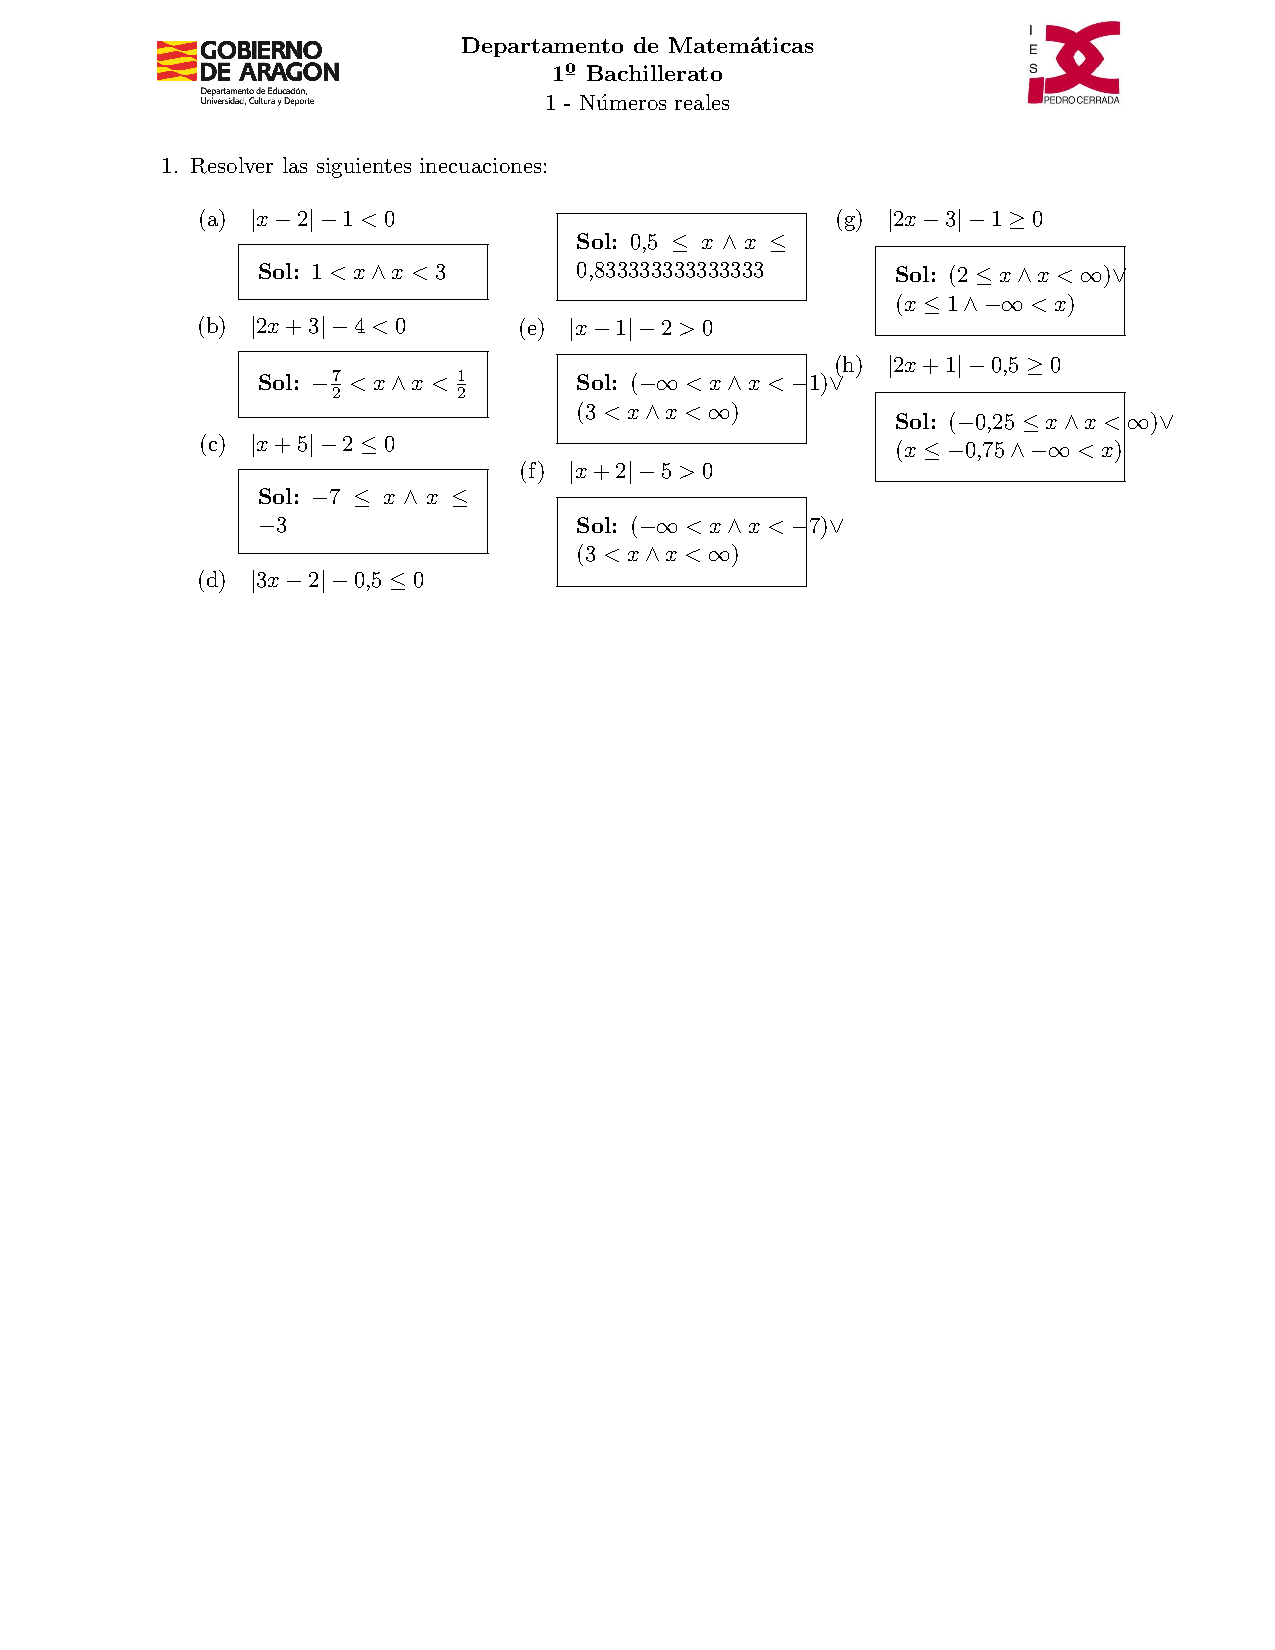
\includepdf[pages=-, scale=0.9]{1_algebra/nreales.pdf}
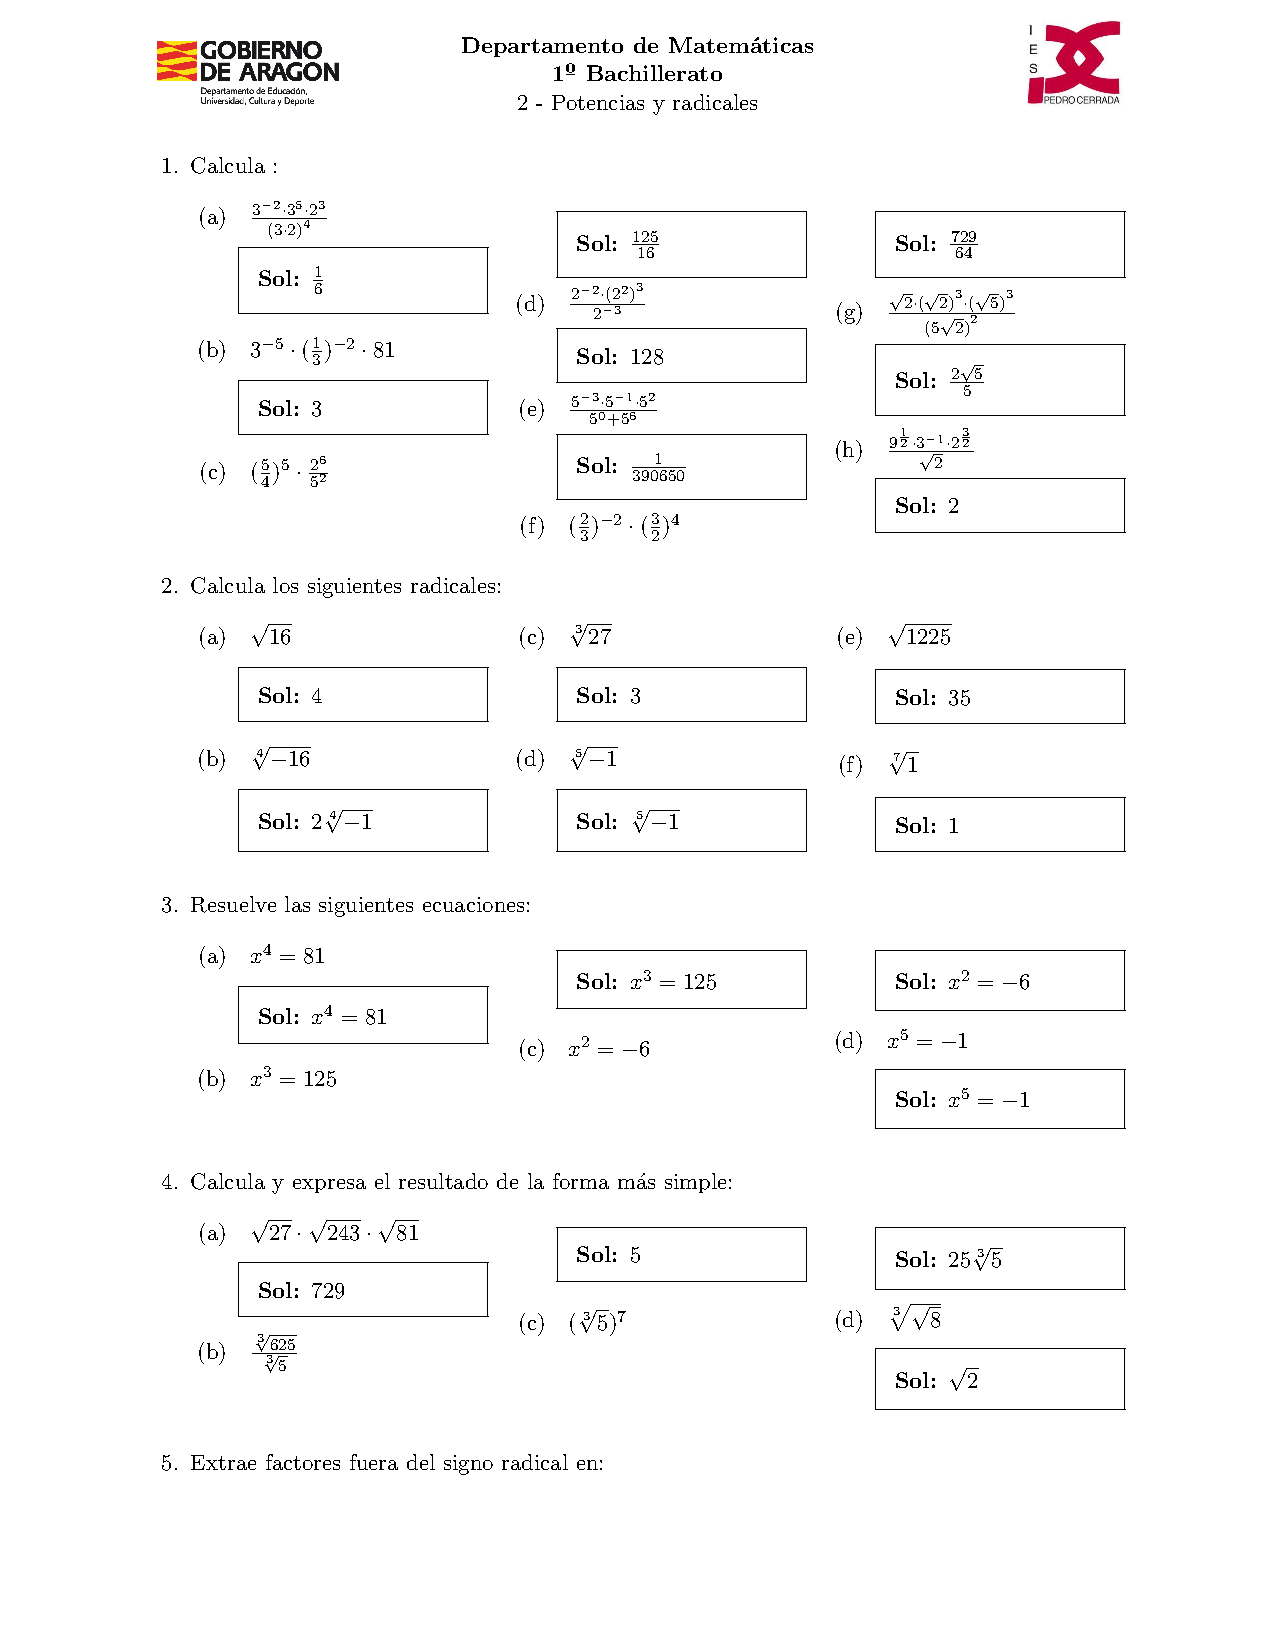
\includepdf[pages=-, scale=0.9]{1_algebra/radicales.pdf}
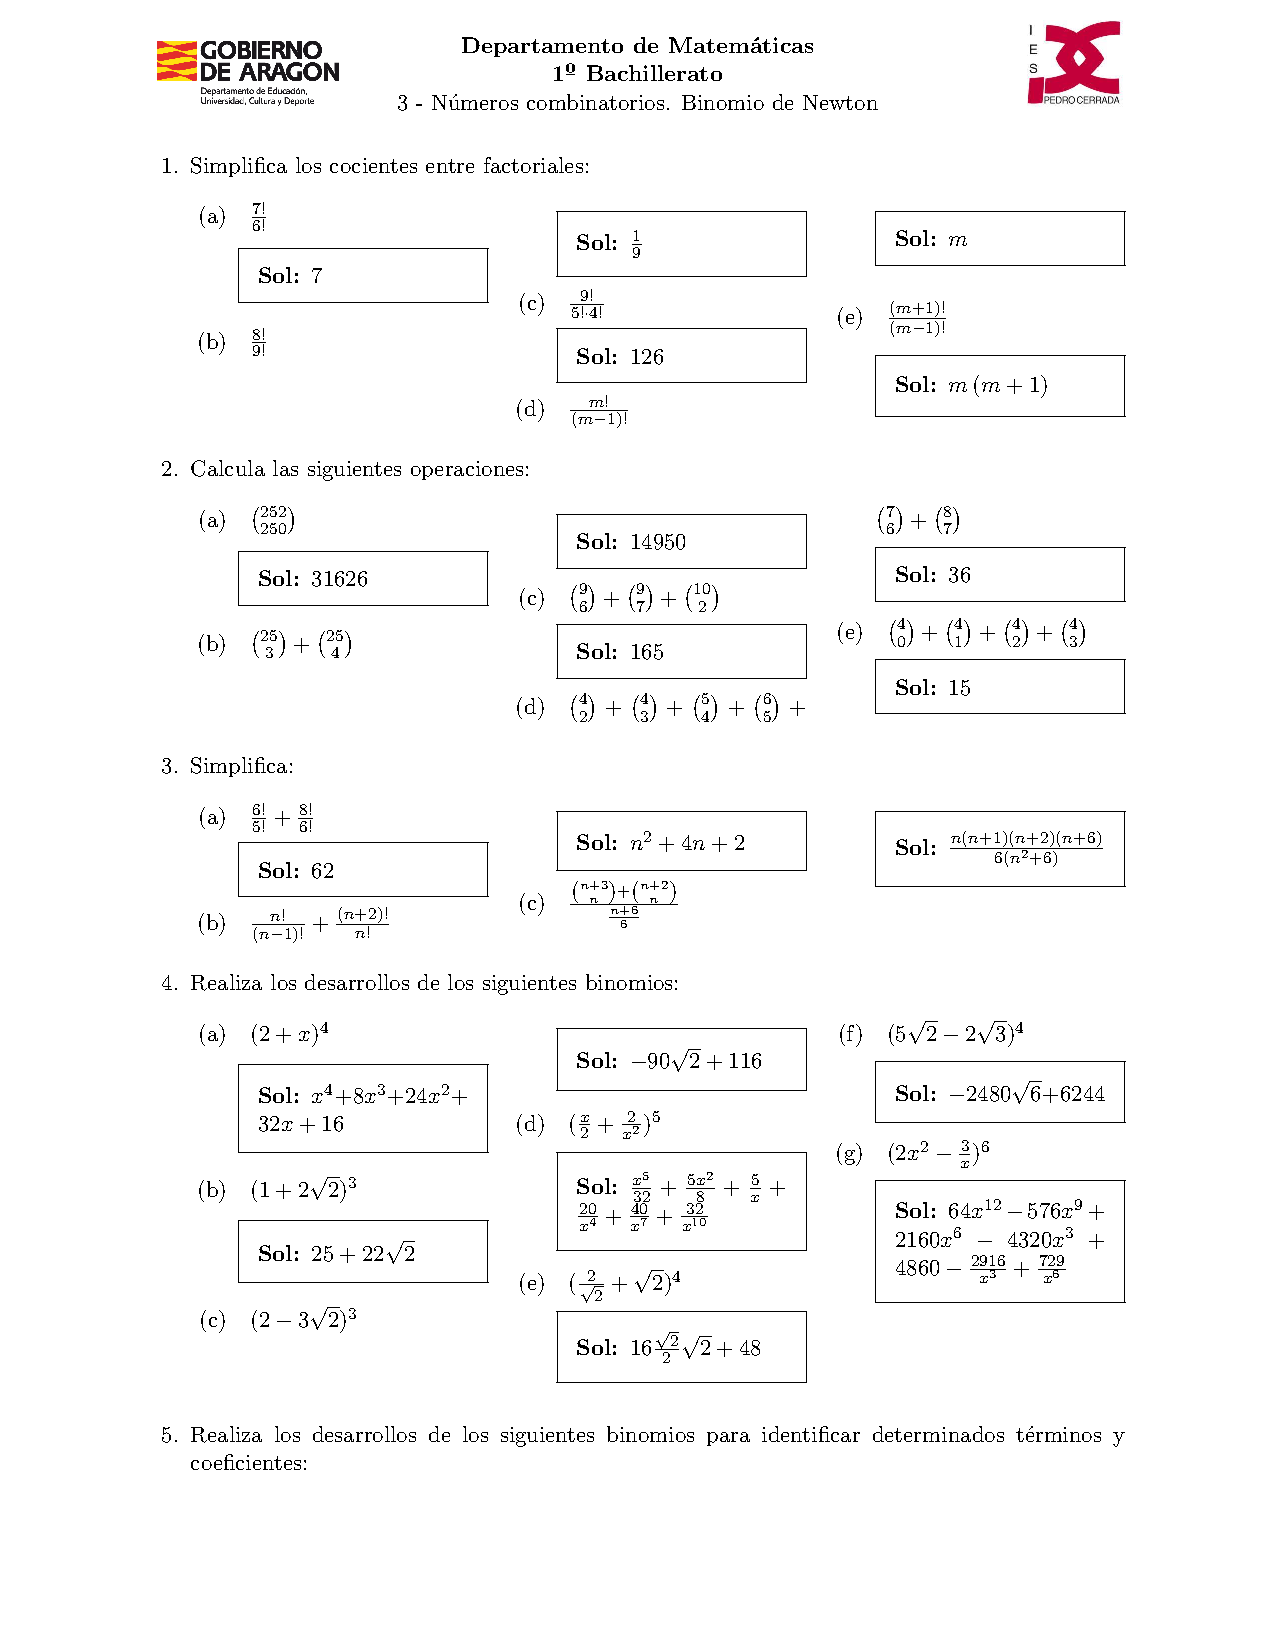
\includepdf[pages=-, scale=0.9]{1_algebra/ncombinatorios.pdf}
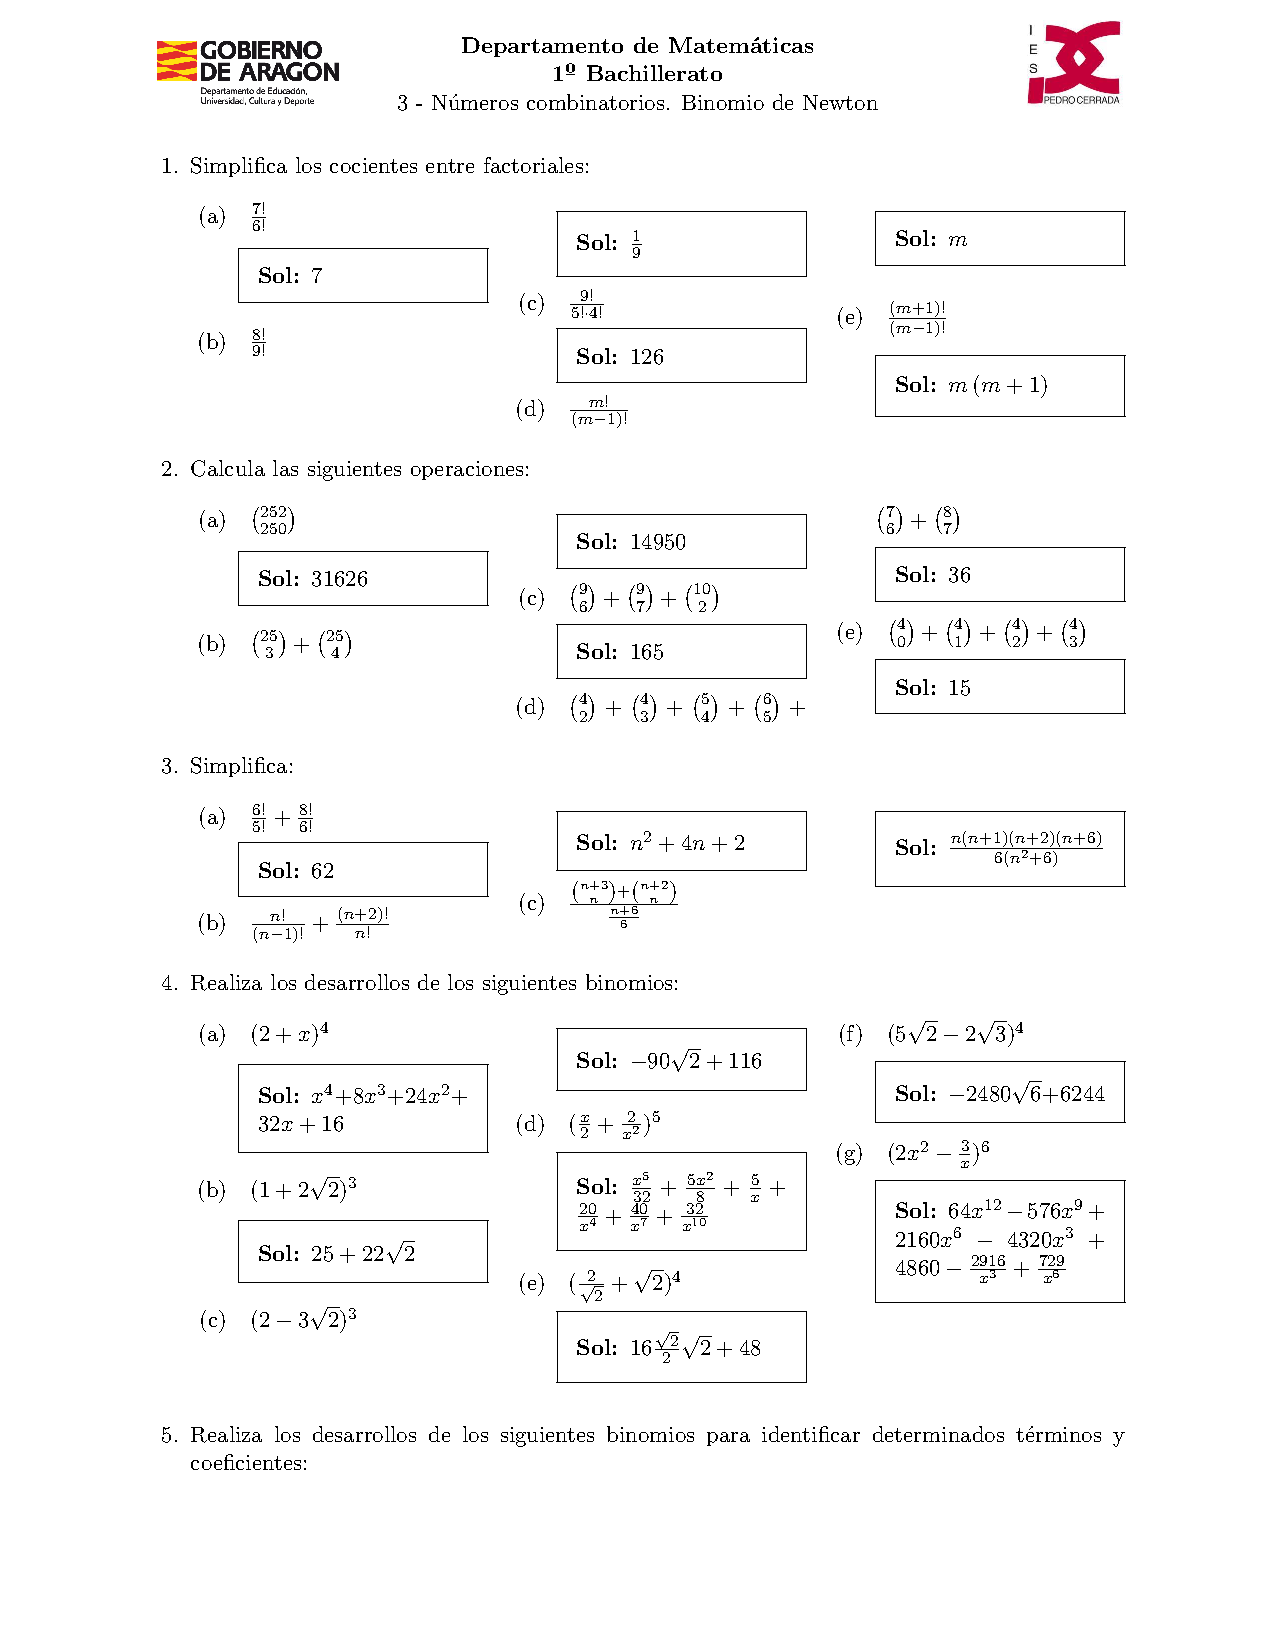
\includepdf[pages=-, scale=0.9]{1_algebra/ncombinatorios.pdf}
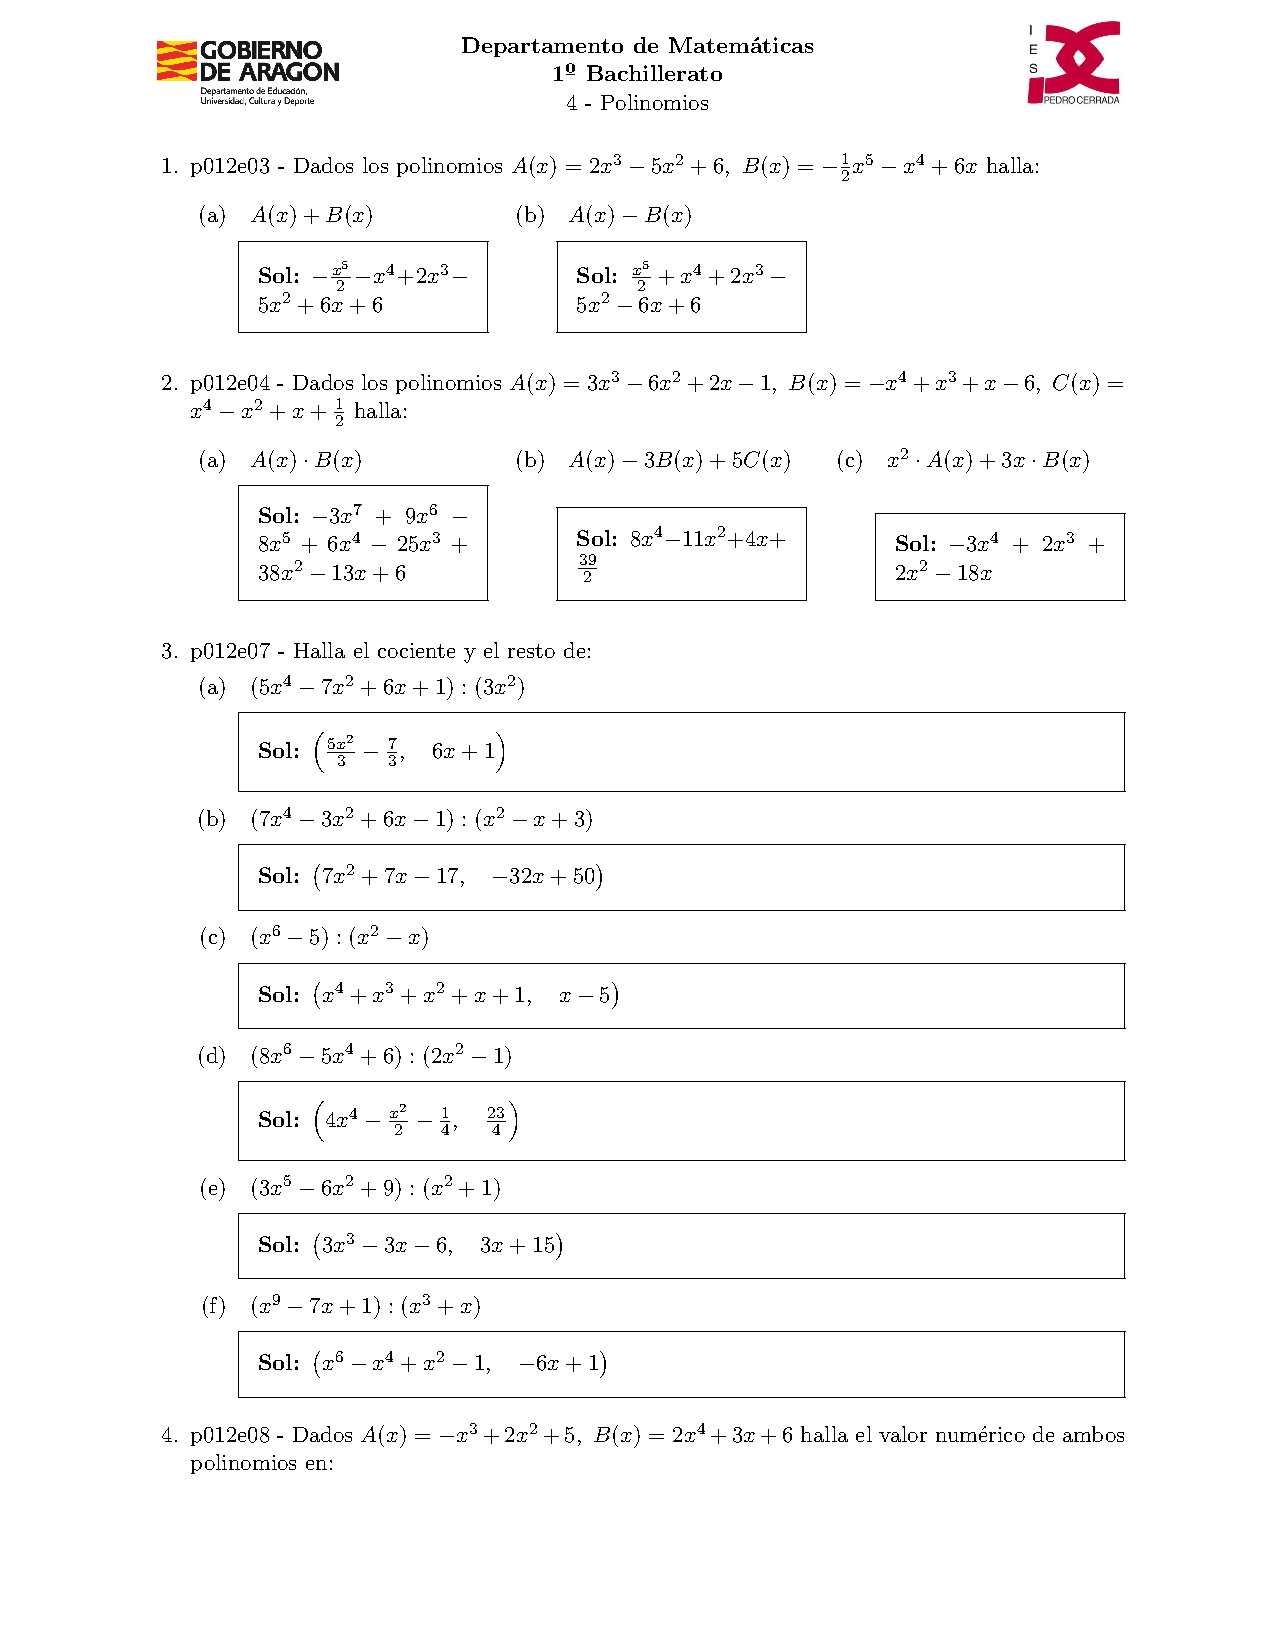
\includepdf[pages=-, scale=0.9]{1_algebra/polinomios.pdf}
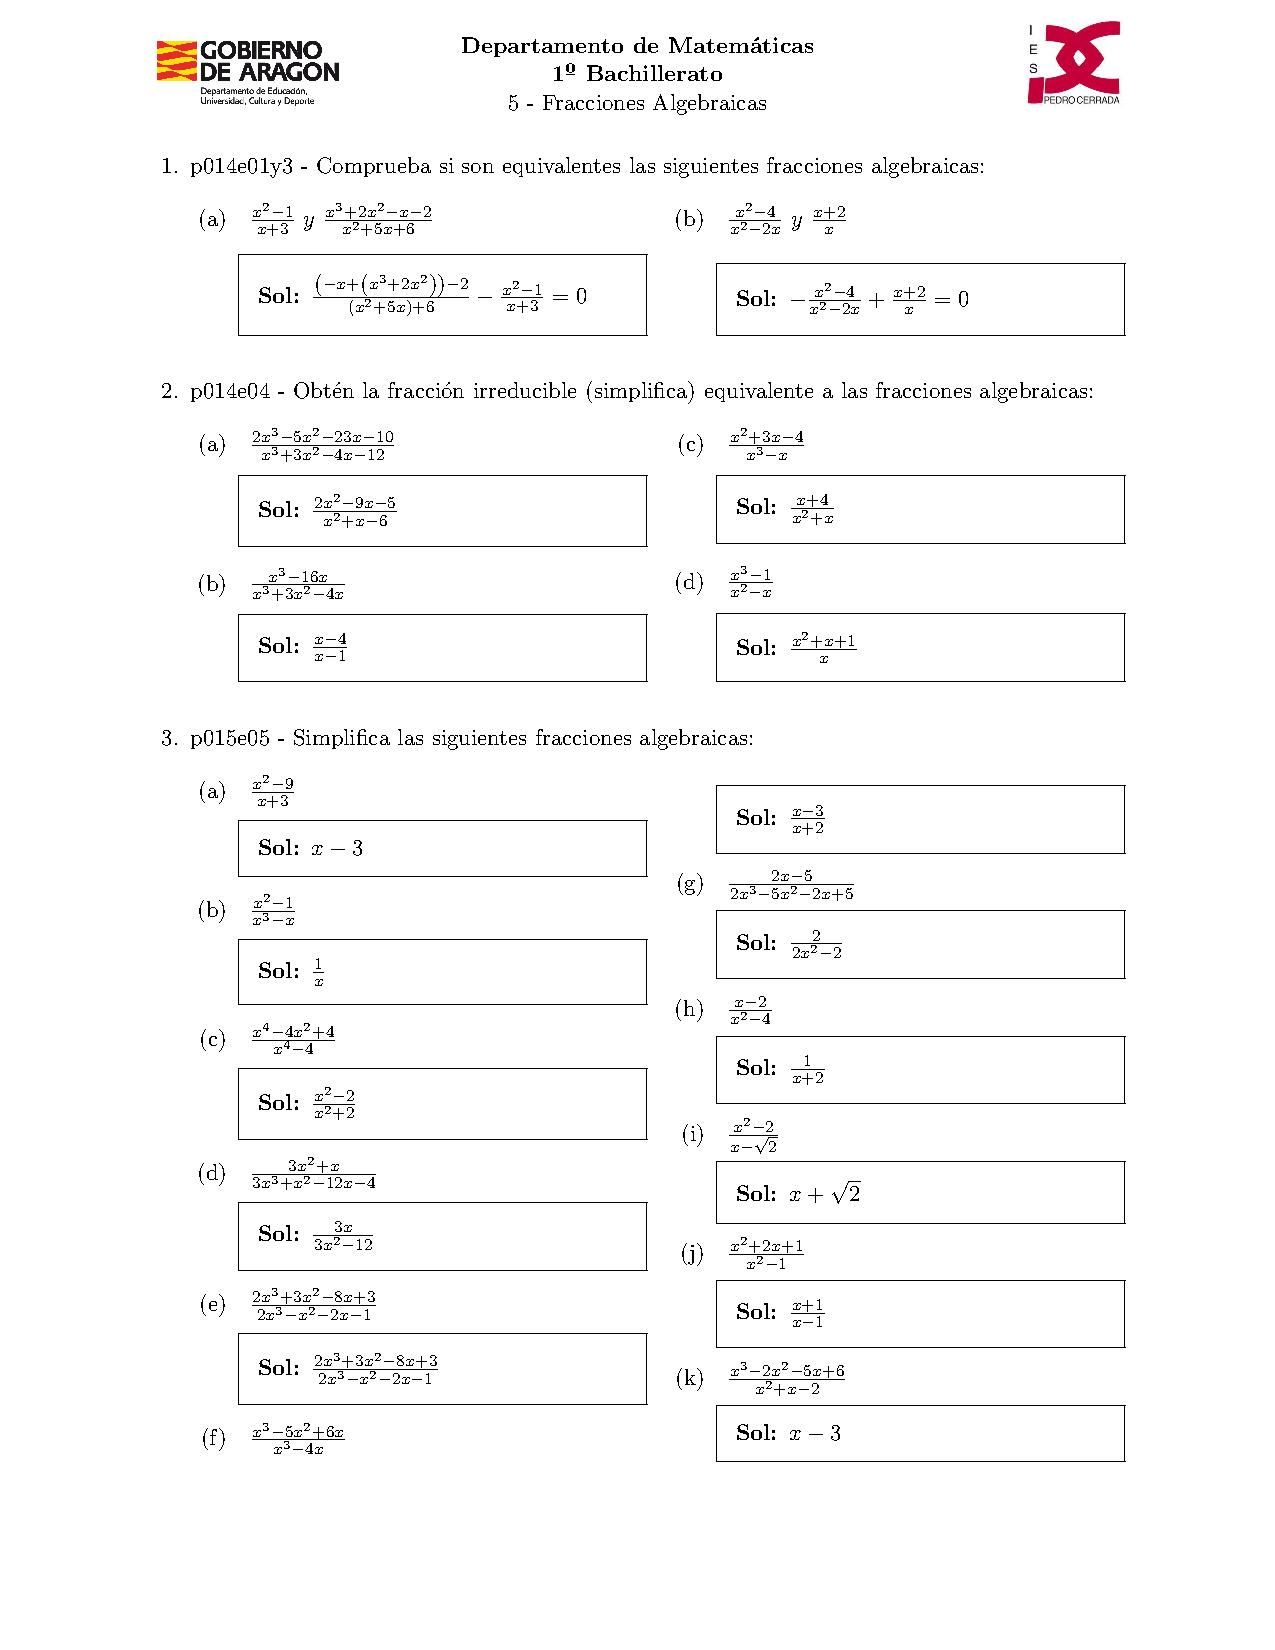
\includepdf[pages=-, scale=0.9]{1_algebra/fraccionesalg.pdf}

\includepdf[pages=-, scale=0.9]{1_algebra/ecuacionesg2.pdf}
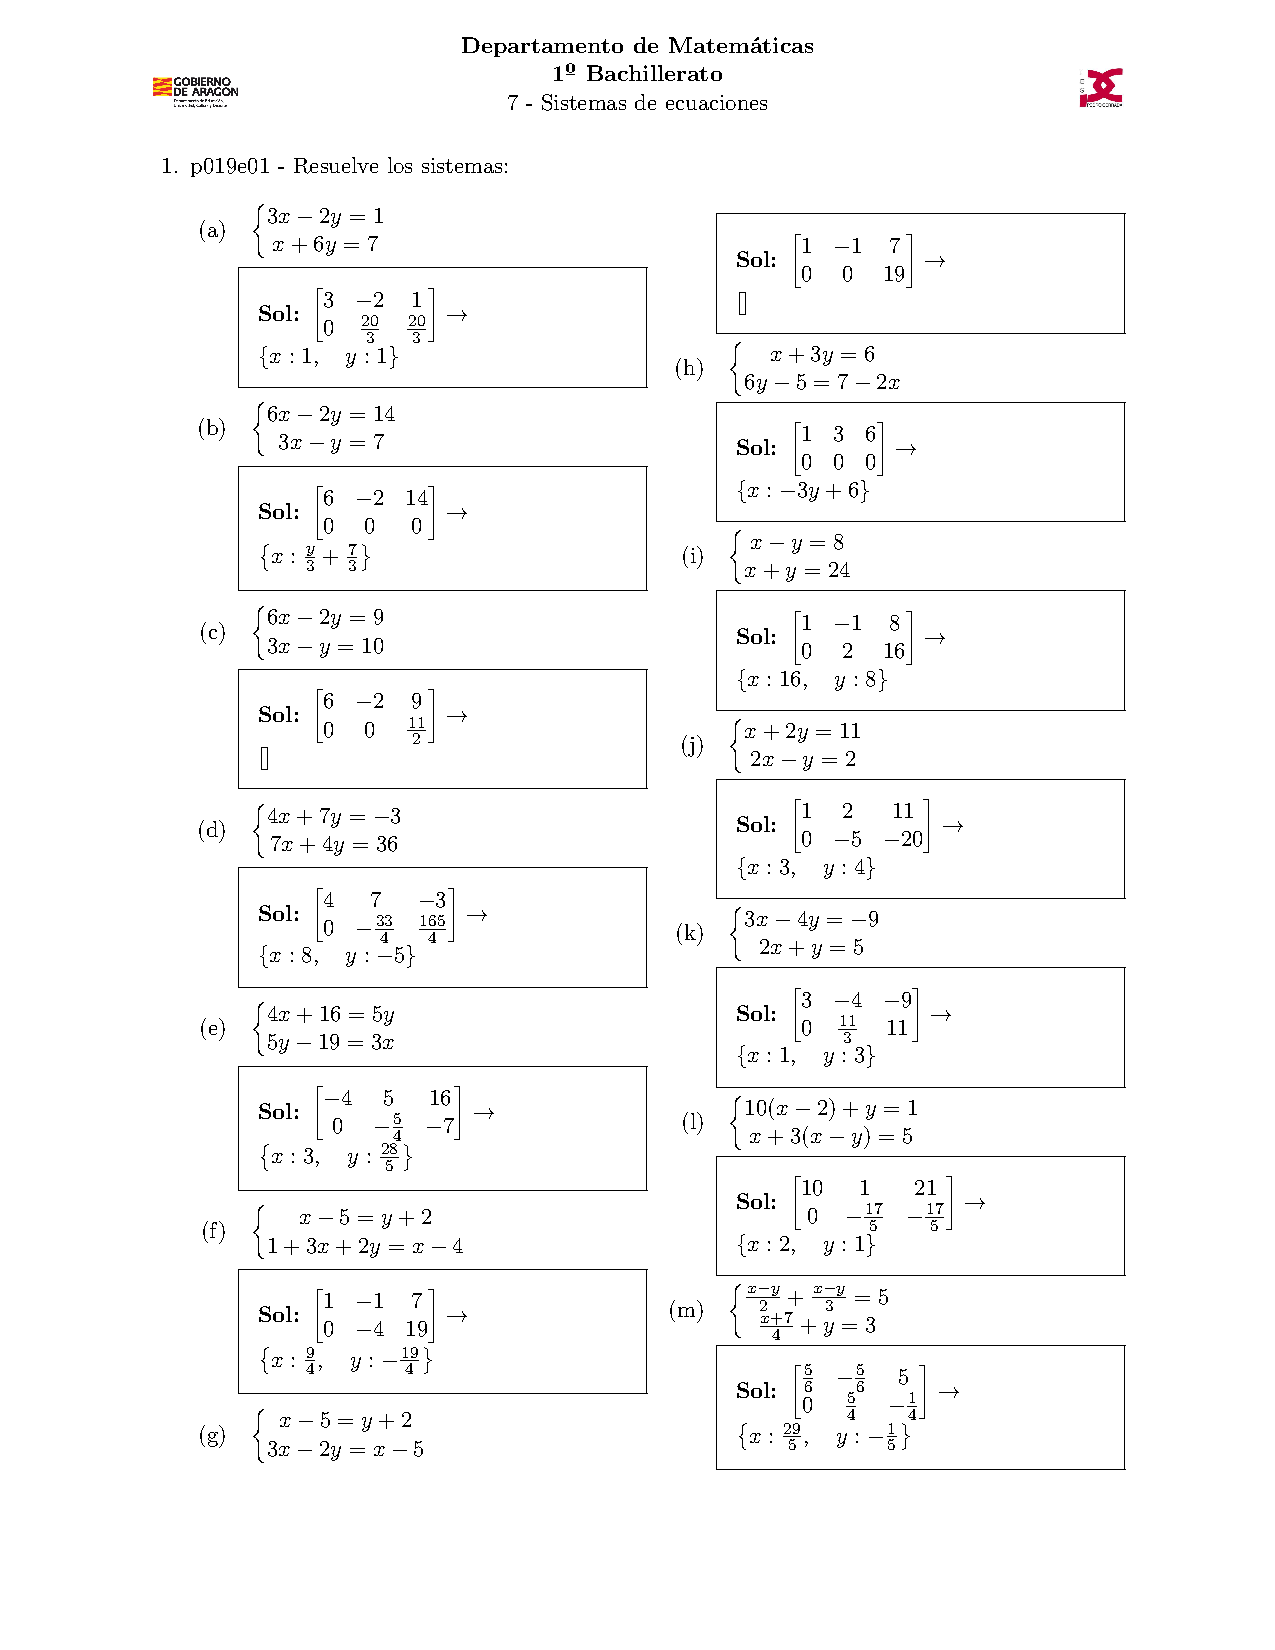
\includepdf[pages=-, scale=0.9]{1_algebra/sistemas_ecuaciones.pdf}
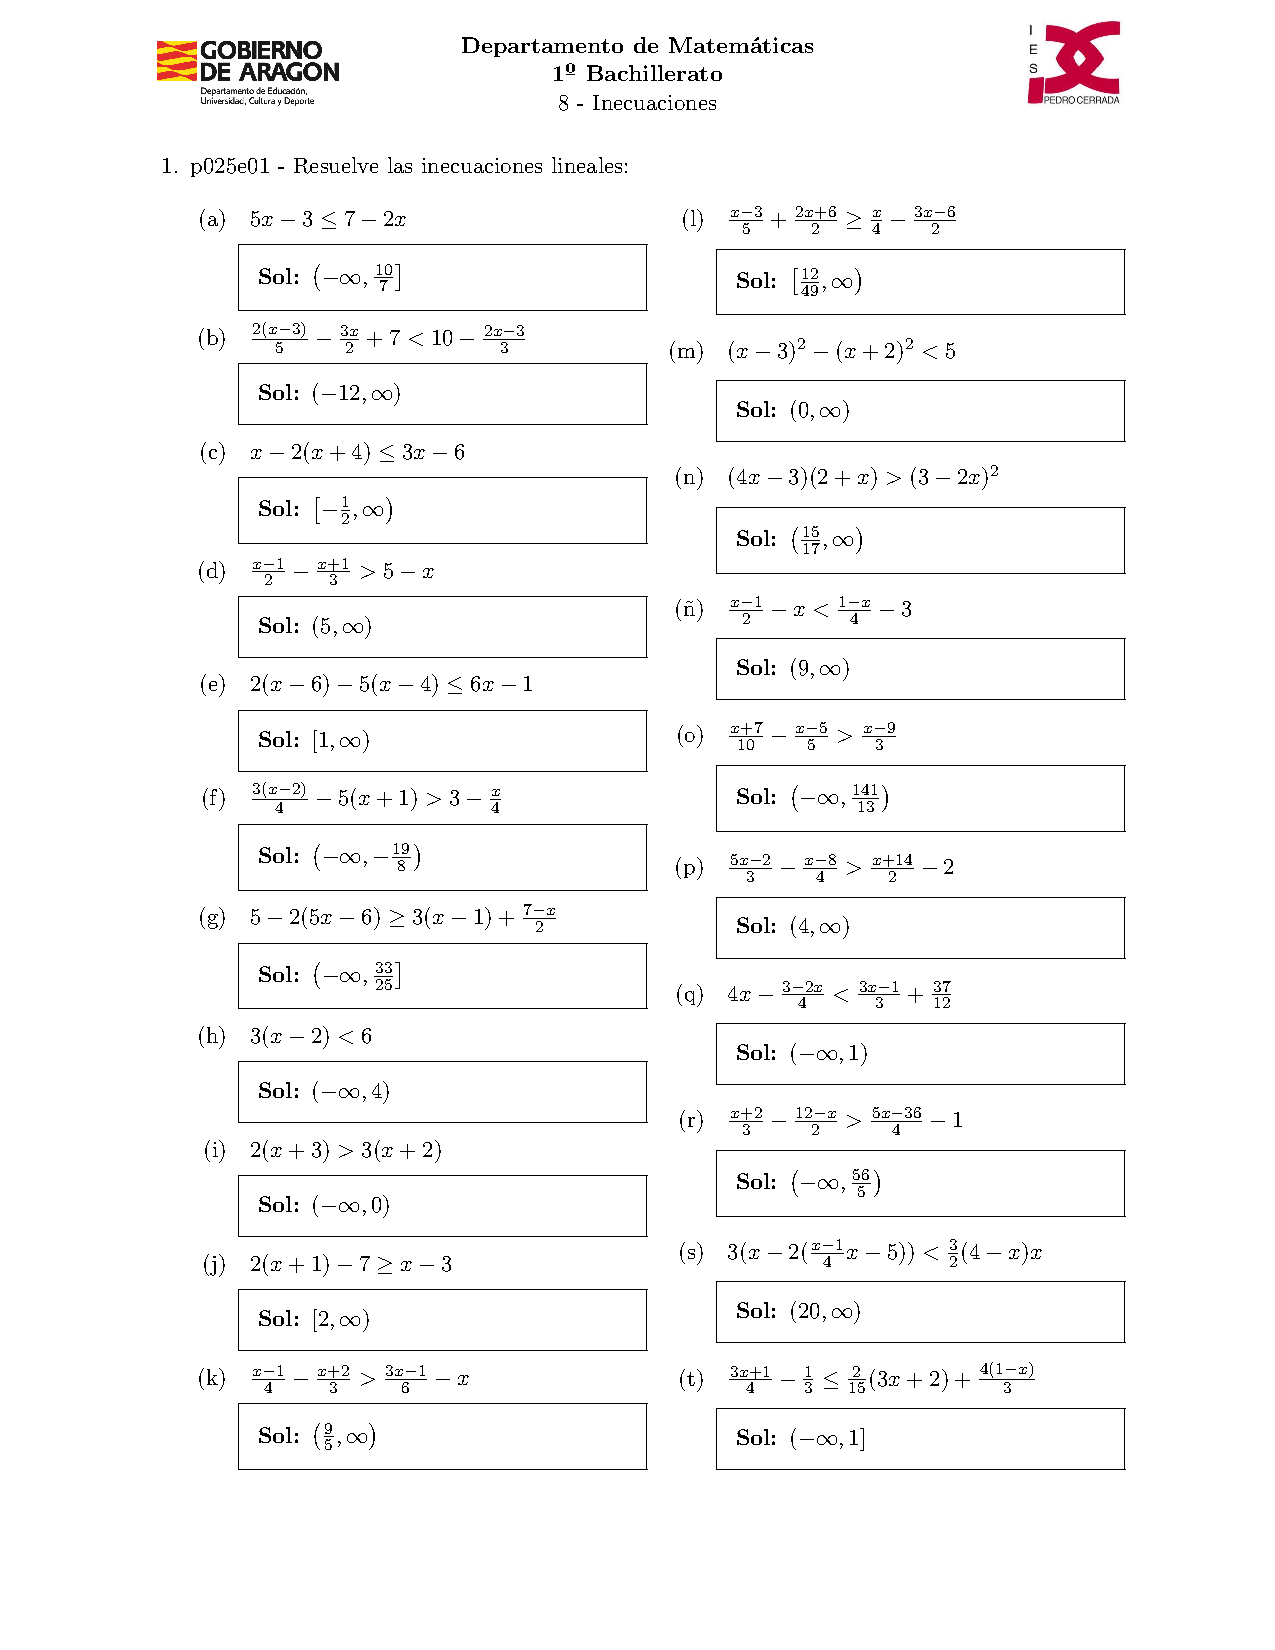
\includepdf[pages=-, scale=0.9]{1_algebra/inecuaciones.pdf}
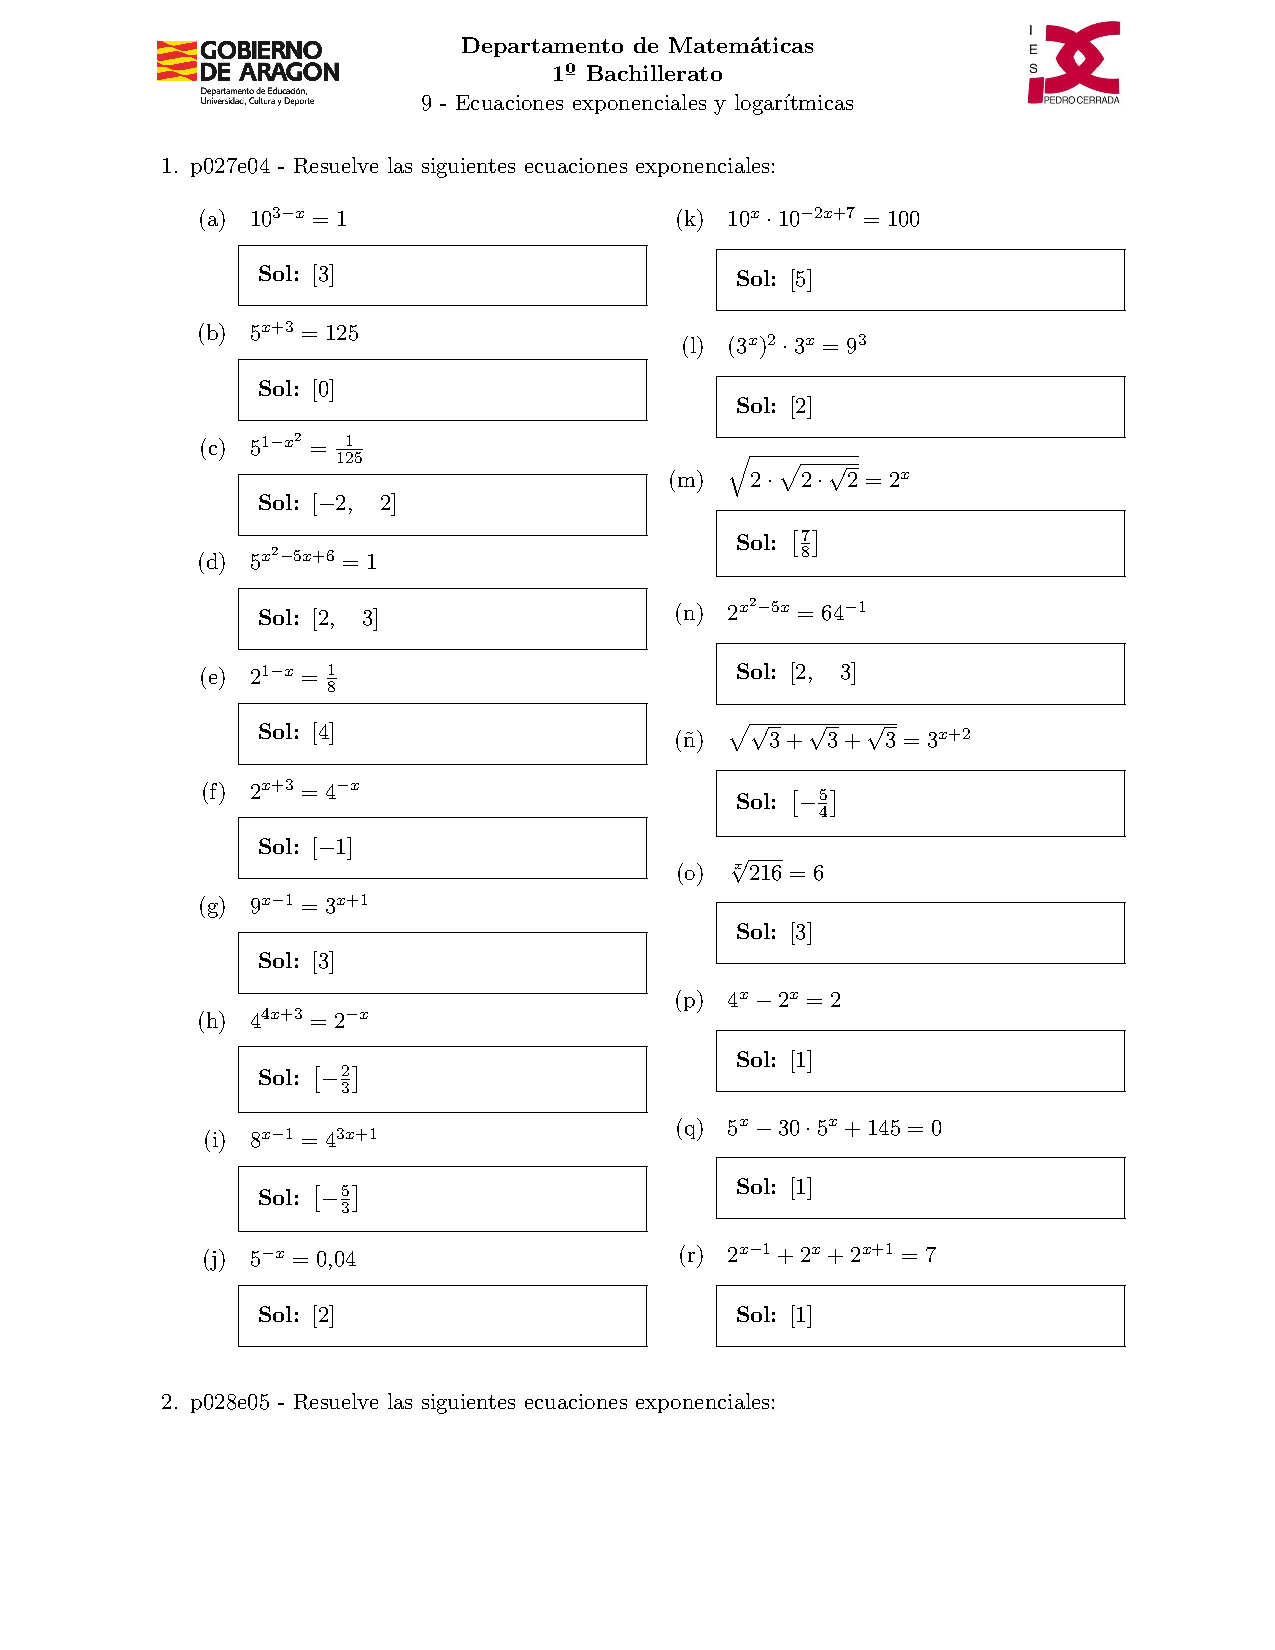
\includepdf[pages=-, scale=0.9]{1_algebra/ecuexplog.pdf}
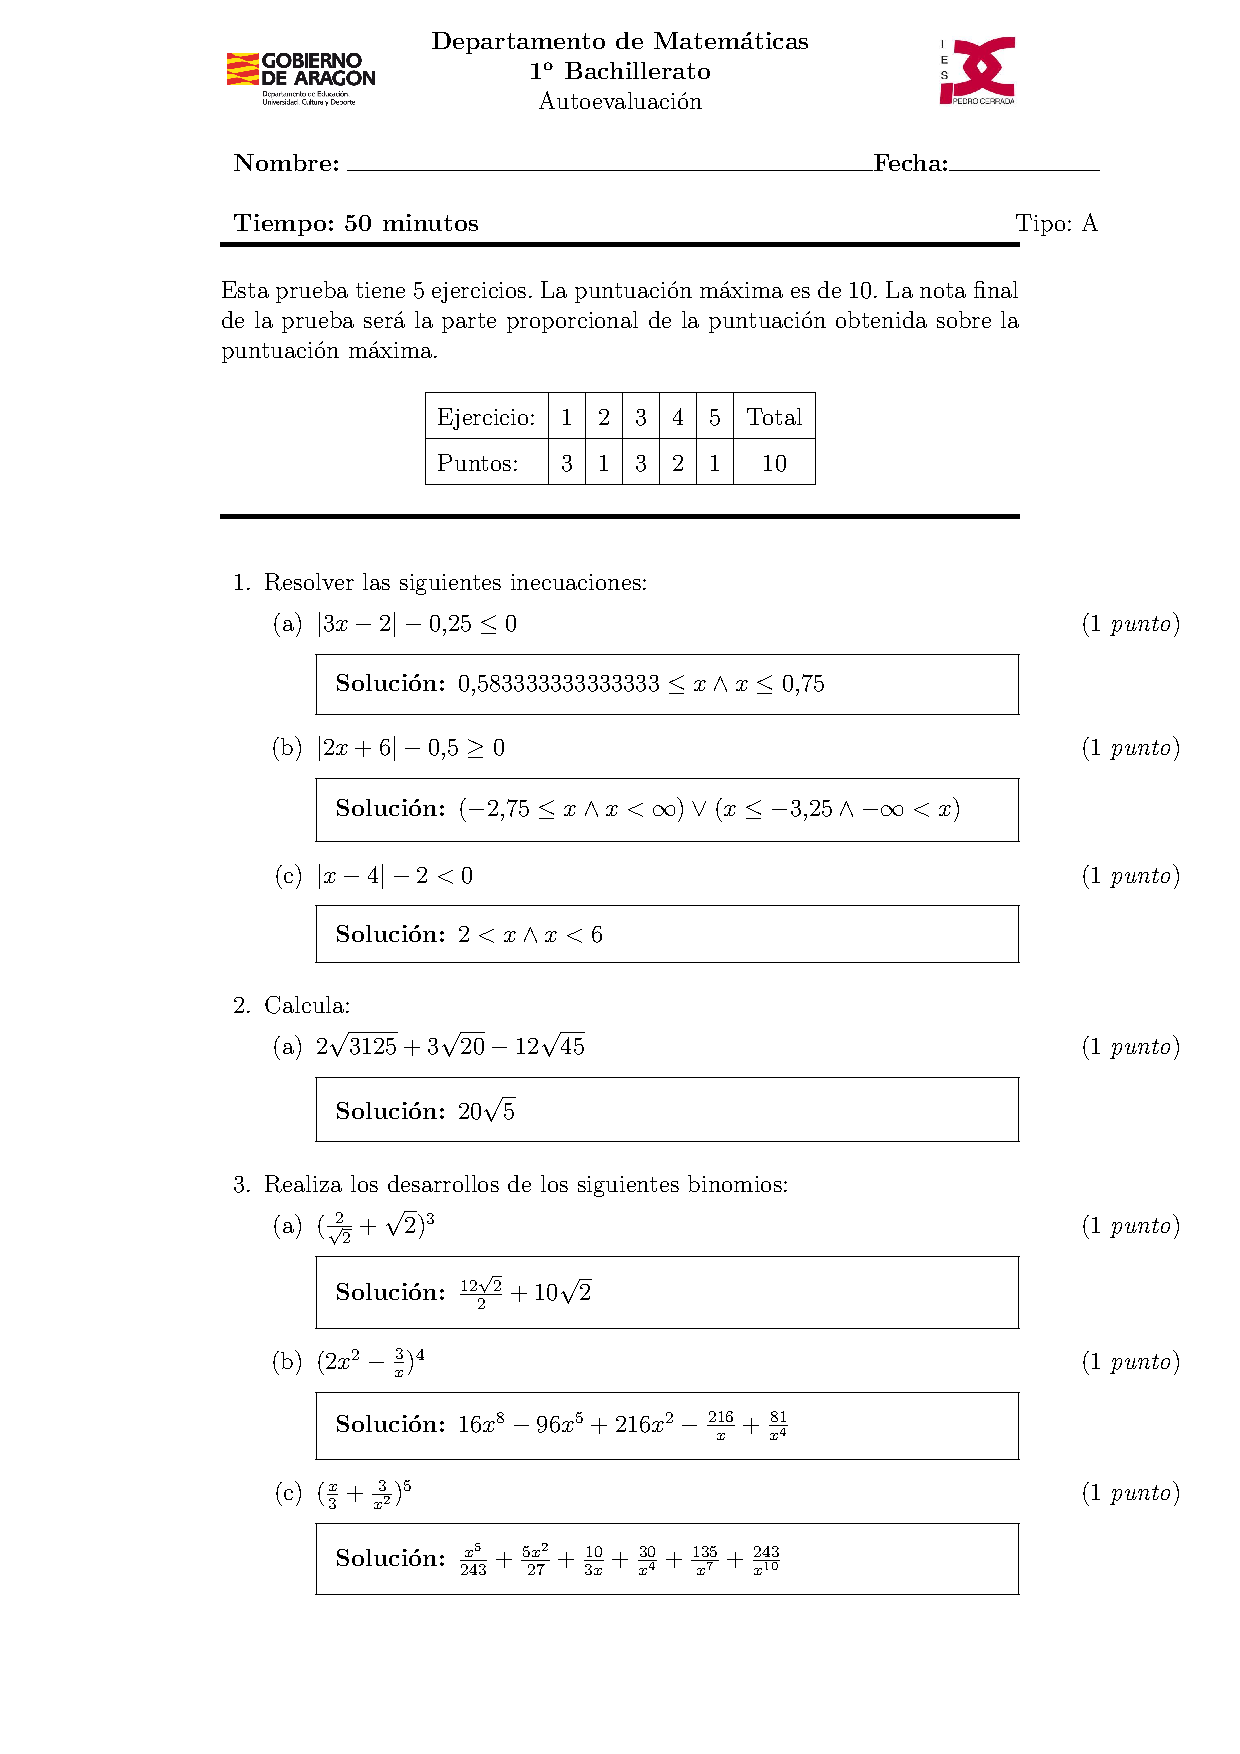
\includepdf[pages=-, scale=0.9]{1_algebra/autoevaluacionA.pdf}
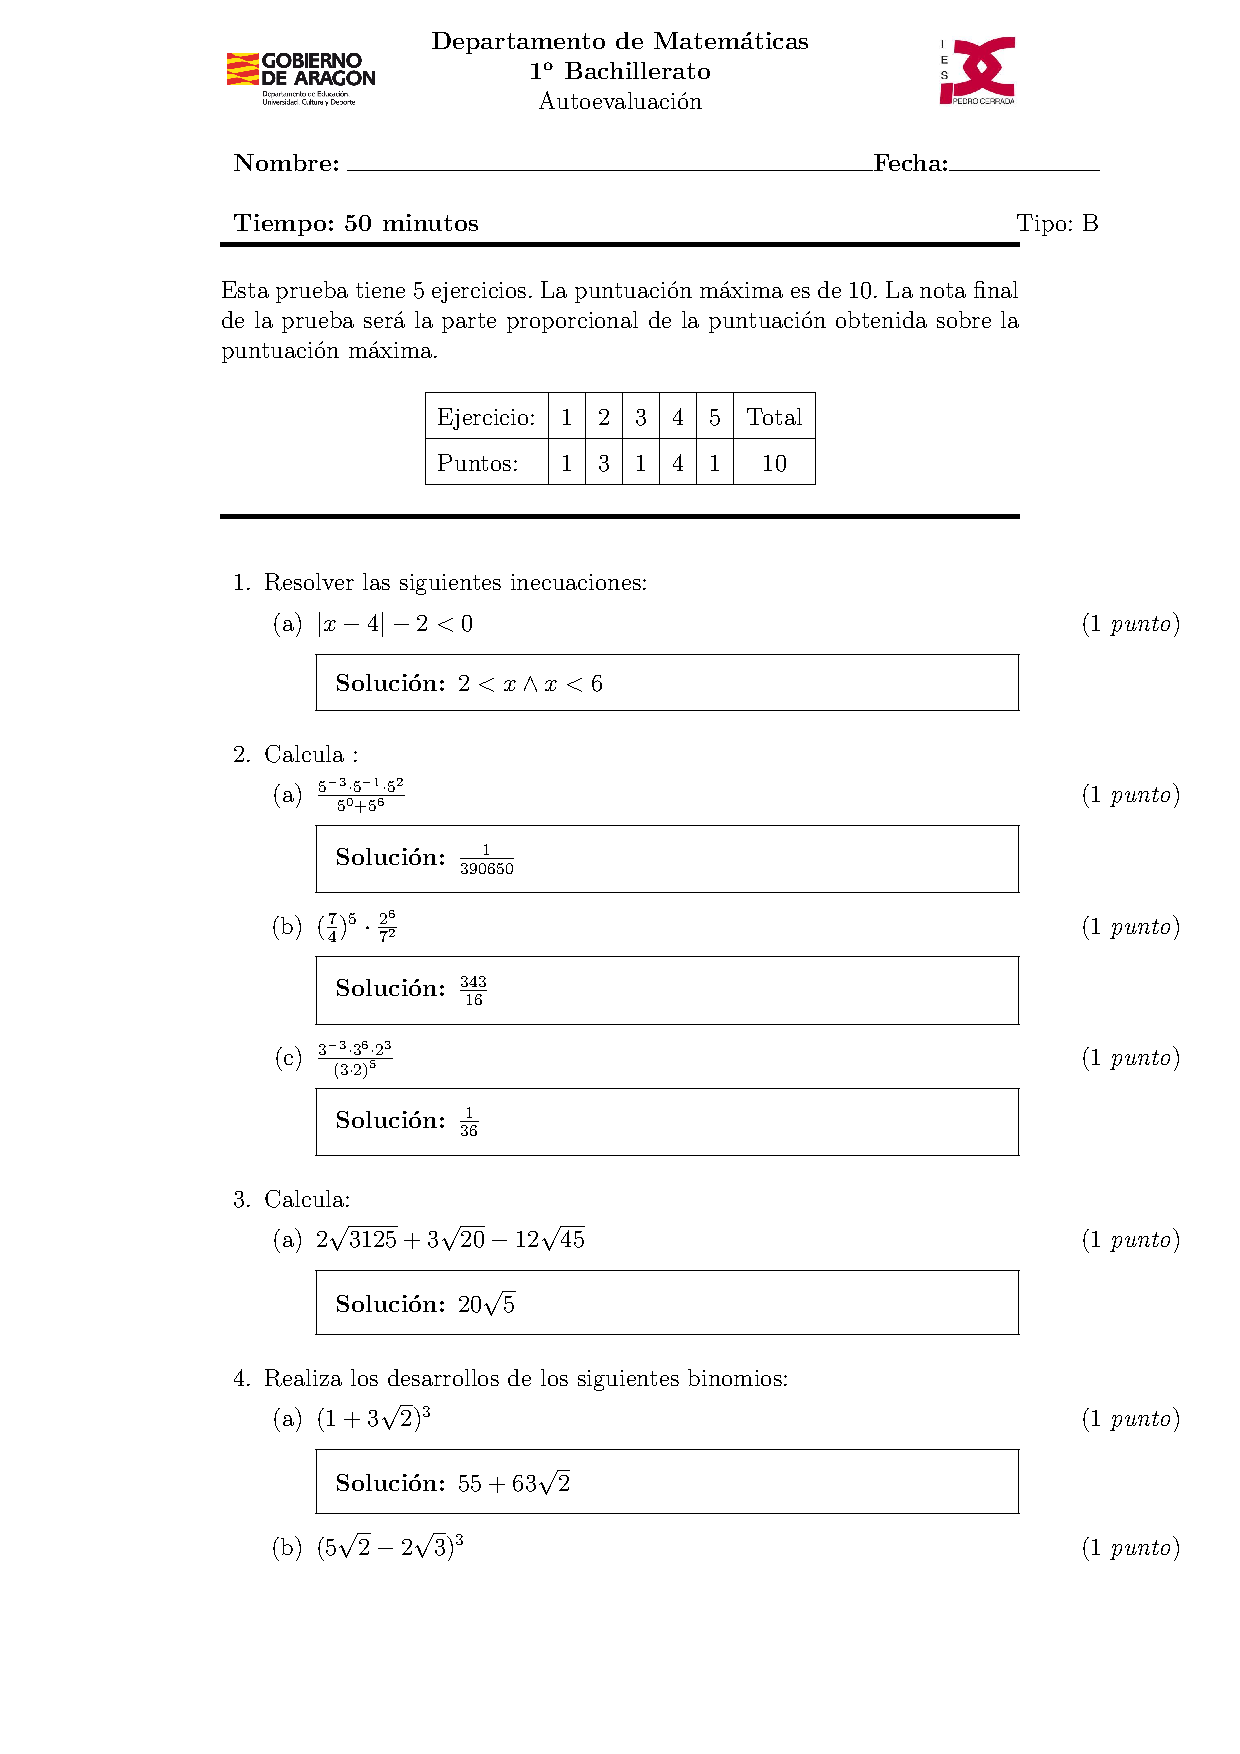
\includepdf[pages=-, scale=0.9]{1_algebra/autoevaluacionB.pdf}
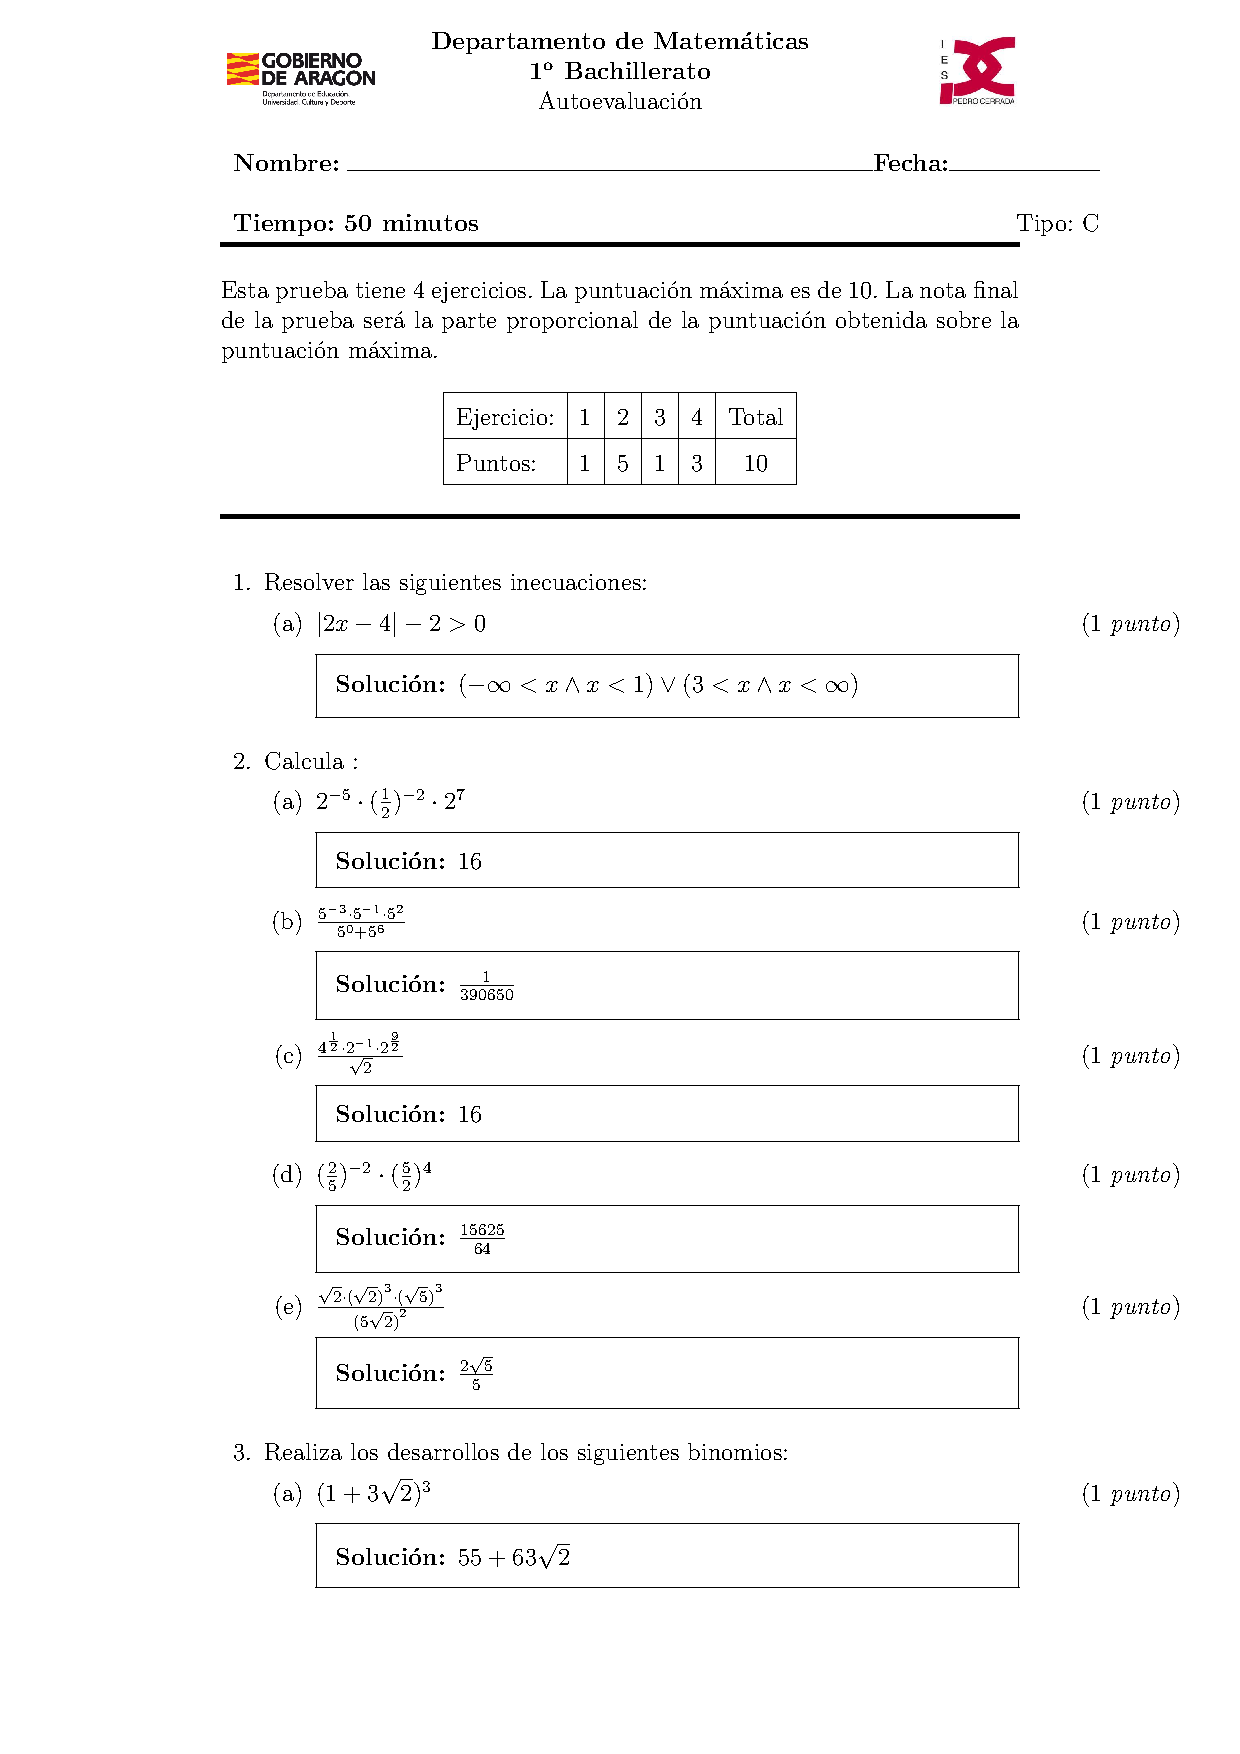
\includepdf[pages=-, scale=0.9]{1_algebra/autoevaluacionC.pdf}






\definecolor{wrwrwr}{rgb}{0.3803921568627451,0.3803921568627451,0.3803921568627451}
\definecolor{rvwvcq}{rgb}{0.98235294117647059,0.396078431372549,0.7529411764705882}
%
%
%
%\begin{tikzpicture}[grow=right, sloped, scale=0.7]\clip(-6.154568000000002,-3.8982211062725844) rectangle (4.2,7);
%\clip(-11.145015598814782,-9.076966577456616) rectangle (18.28831648795786,8.422371196936597);
%\fill[line width=2pt,color=red,fill=rvwvcq,fill opacity=0.00000000149011612] (-5,-1) -- (3,-1) -- (0,6) -- cycle;
%\draw[line width=1.6pt,fill=black,fill opacity=0.10000000149011612] (-2.616480014189626,2.336927980134524) -- (-2.1696242105403662,2.0177452632421953) -- (-1.8504414936480373,2.464601066891455) -- (-2.2972972972972974,2.7837837837837838) -- cycle; 
%\draw[line width=1.6pt,fill=black,fill opacity=0.10000000149011612] (1.5423027784864105,2.401293516865042) -- (1.0375609857592993,2.1849756056962804) -- (1.2538788969280612,1.6802338129691692) -- (1.7586206896551724,1.896551724137931) -- cycle; 
%\draw[line width=1.6pt,fill=black,fill opacity=0.10000000149011612] (0.5491427100652383,-1) -- (0.5491427100652384,-0.4508572899347618) -- (0,-0.4508572899347617) -- (0,-1) -- cycle; 
%\draw [line width=2pt,color=rvwvcq] (-5,-1)-- (3,-1);
%\draw [line width=2pt,color=rvwvcq] (3,-1)-- (0,6);
%\draw [line width=2pt,color=rvwvcq] (0,6)-- (-5,-1);
%\draw [line width=2pt,color=wrwrwr] (0,-9.076966577456616) -- (0,8.422371196936597);
%\draw [line width=2pt,color=wrwrwr,domain=-11.145015598814782:18.28831648795786] plot(\x,{(-8-3*\x)/-7});
%\draw [line width=2pt,color=wrwrwr,domain=-11.145015598814782:18.28831648795786] plot(\x,{(--8-5*\x)/7});
%\begin{scriptsize}
%\draw [fill=rvwvcq] (-5,-1) circle (2.5pt);
%\draw[color=rvwvcq] (-4.802740874752074,-0.42299719371372185) node {$A$};
%\draw [fill=rvwvcq] (3,-1) circle (2.5pt);
%\draw[color=rvwvcq] (3.1962913282494623,-0.42299719371372185) node {$B$};
%\draw [fill=rvwvcq] (0,6) circle (2.5pt);
%\draw[color=rvwvcq] (0.21930523328125284,6.576737916043563) node {$C$};
%\draw[color=black] (-1.0750365471397076,2.530016055715133) node {$\alpha = 90\textrm{\degre}$};
%\draw[color=black] (2.3937994243884666,2.256588902990239) node {$\beta = 90\textrm{\degre}$};
%\draw[color=black] (1.4877601780937941,-0.4776826242587007) node {$\gamma = 90\textrm{\degre}$};
%\draw [fill=wrwrwr] (0,1.1428571428571428) circle (2pt);
%\draw[color=wrwrwr] (1.8501758766116632,1.1355375768181737) node {$Ortocentro$};
%\end{scriptsize}
%\end{tikzpicture}
%
%\begin{tikzpicture}[line cap=round,line join=round,>=triangle 45,x=1cm,y=1cm, scale=0.8]
%\draw [color=lightgray,dash pattern=on 1pt off 1pt, xstep=1cm,ystep=1cm] (-0.6129302567150502,-0.43158220601634095) grid (9.010648940148005,6.1);
%\draw[->,color=black] (-0.6129302567150502,0) -- (9.010648940148005,0);
%\foreach \x in {,1,2,3,4,5,6,7,8,9}
%\draw[shift={(\x,0)},color=black] (0pt,2pt) -- (0pt,-2pt) node[below] {\footnotesize $\x$};
%\draw[->,color=black] (0,-0.43158220601634095) -- (0,6.1);
%\foreach \y in {,1,2,3,4,5,6}
%\draw[shift={(0,\y)},color=black] (2pt,0pt) -- (-2pt,0pt) node[left] {\footnotesize $\y$};
%\draw[color=black] (0pt,-10pt) node[right] {\footnotesize $0$};
%\clip(-0.6129302567150502,-0.43158220601634095) rectangle (9.010648940148005,7.8783927087822985);
%\draw [->,line width=1.5pt,color=red] (1,1) -- node[above,fill=white]{$\overrightarrow{v}=\left(6,4 \right) \land \left|\overrightarrow{v}\right|=\sqrt{6^2+4^2}=\sqrt{52}$} (7,5);
%\draw [-,line width=2pt,color=blue] (1,1) -- node[below]{$7-1=6$} (7,1);
%\draw [-,line width=2pt,color=orange] (7,1) -- node[right]{$5-1=4$}(7,5);
%
%\draw [fill=yellow, color=blue]  (1,1) circle (2pt) node[above] {$A = (1, 1)$};
%\draw [fill=yellow, color=blue]  (7,5) circle (2pt) node[above] {$B = (7, 5)$};
%\end{tikzpicture}
%%\input{geometria_analitica}

%\input{geometria/geometria_analitica}

\chapter{Geometría}

%\input{analisis/funciones}


\includepdf[pages=-, scale=0.9]{2_geometria/teorver.pdf}
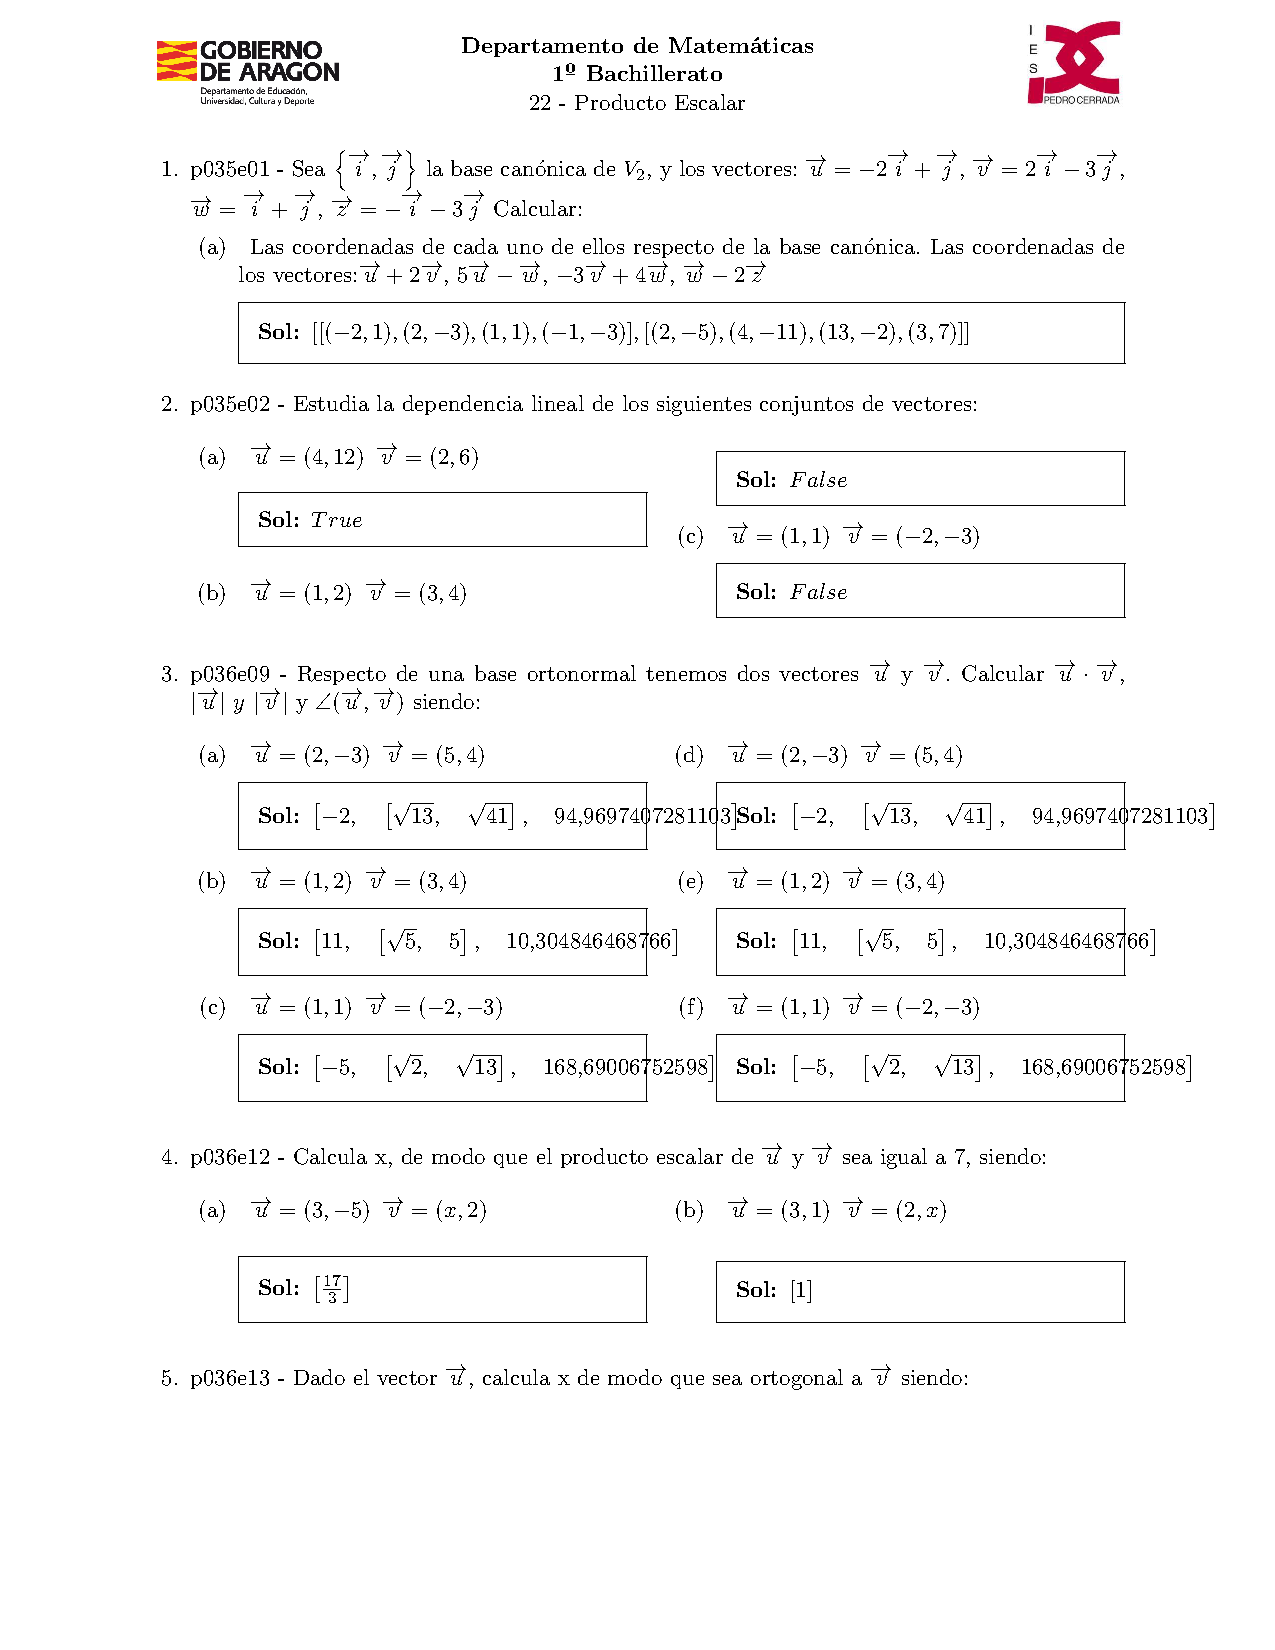
\includepdf[pages=-, scale=0.9]{2_geometria/prodesc.pdf}
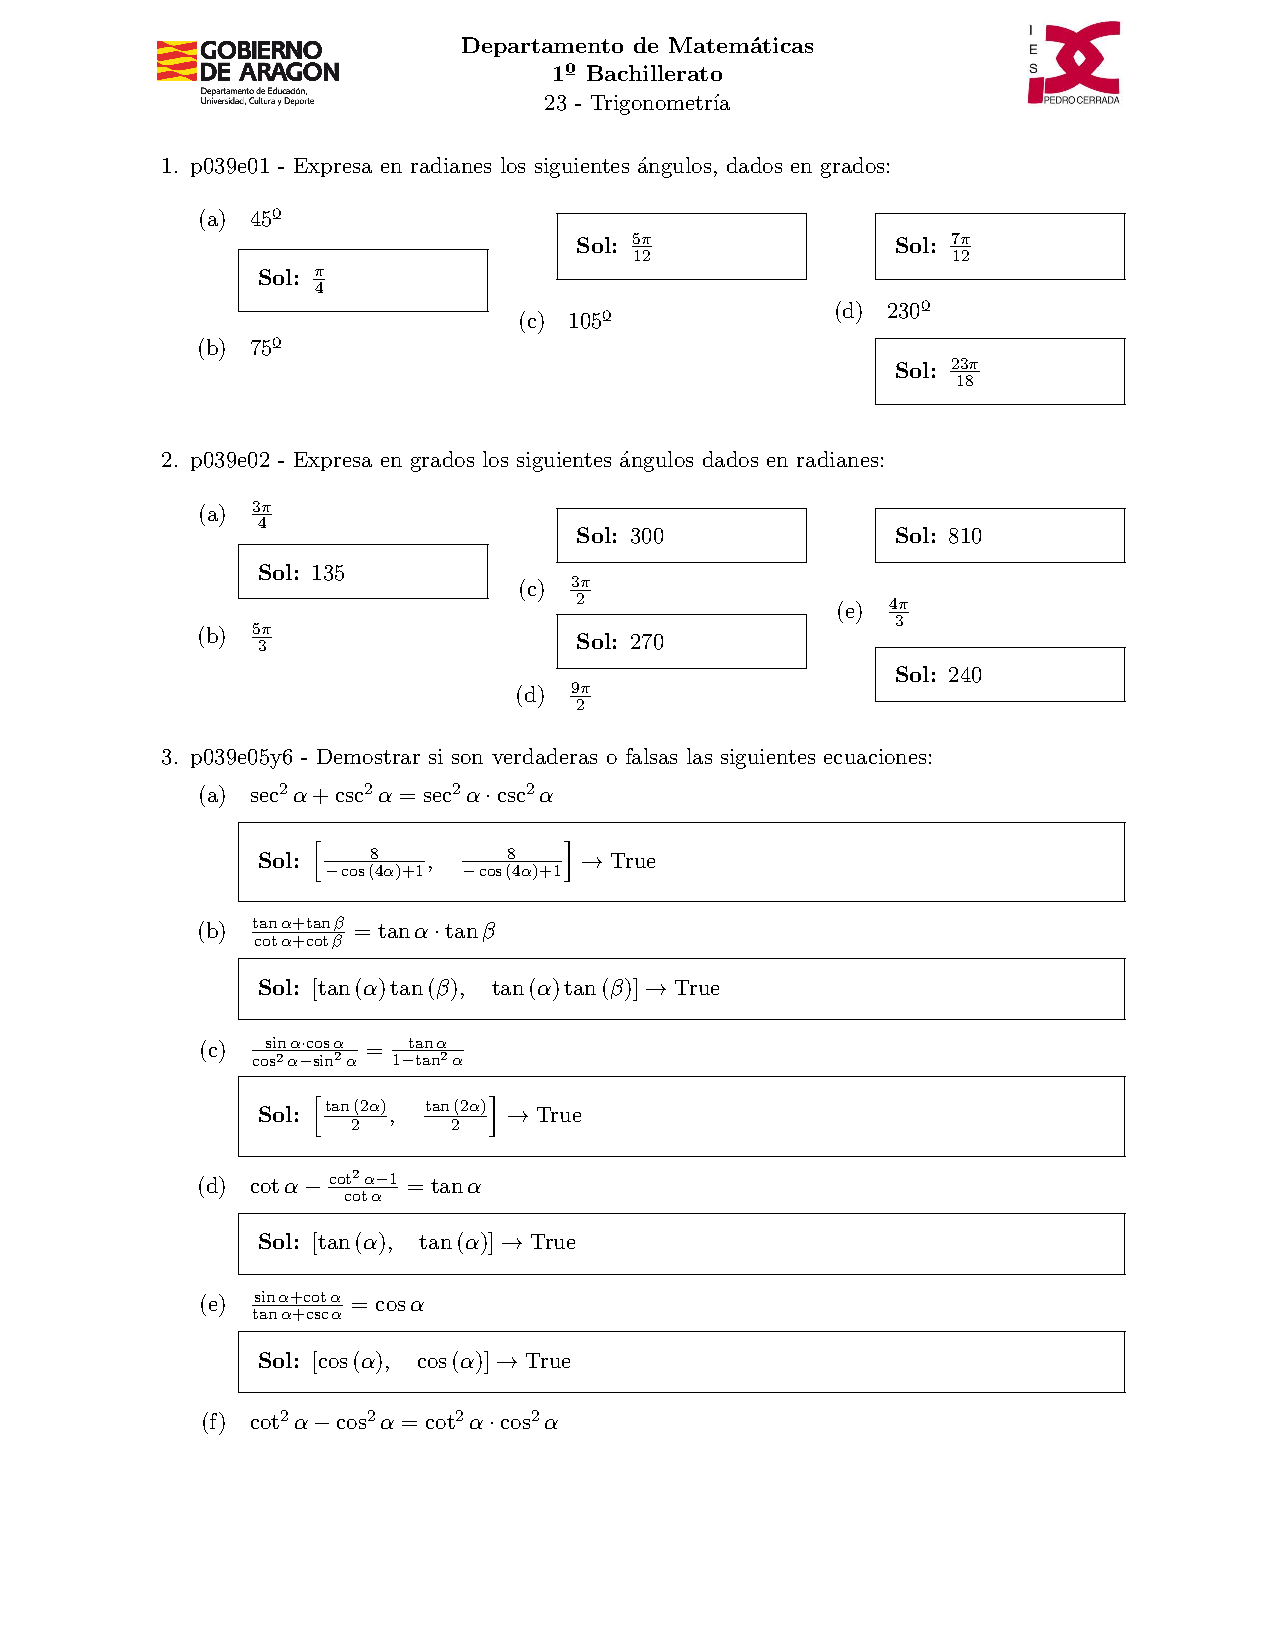
\includepdf[pages=-, scale=0.9]{2_geometria/trigono.pdf}
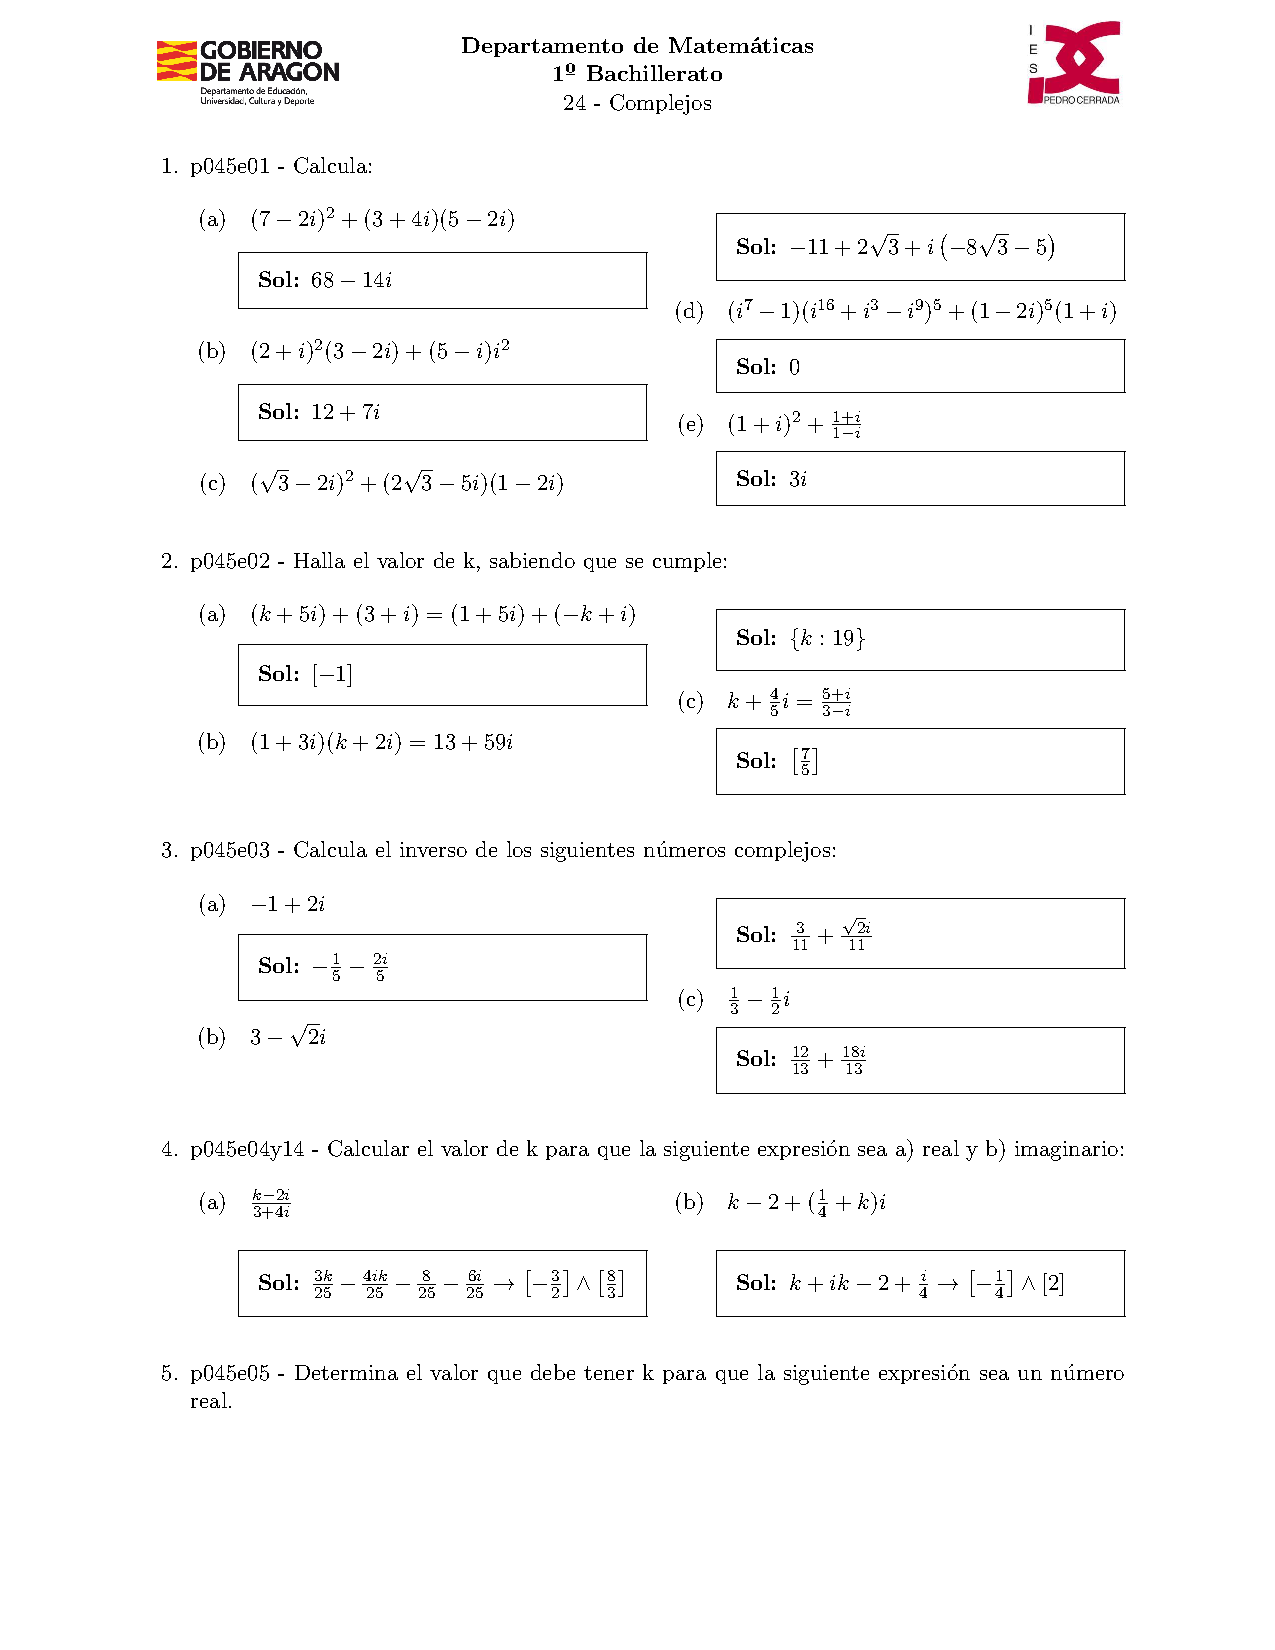
\includepdf[pages=-, scale=0.9]{2_geometria/complejos.pdf}
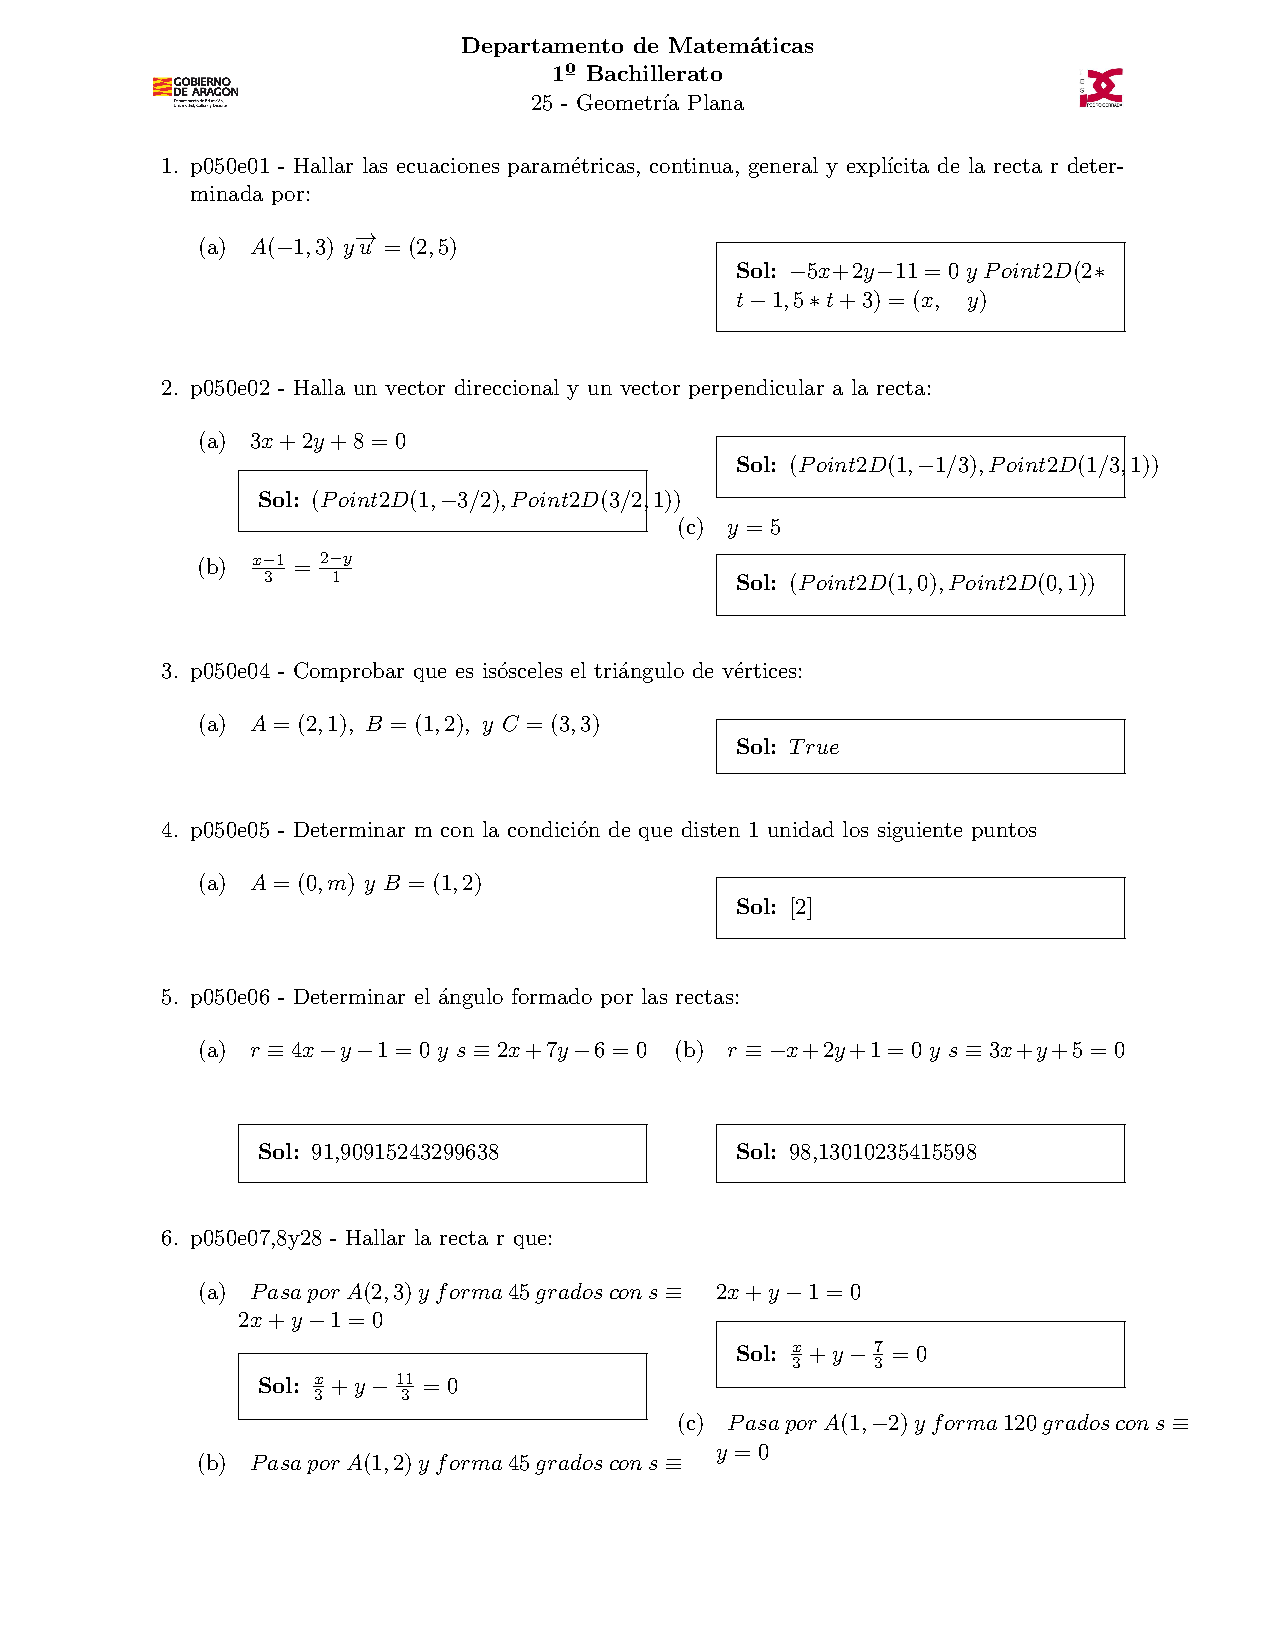
\includepdf[pages=-, scale=0.9]{2_geometria/geopla.pdf}
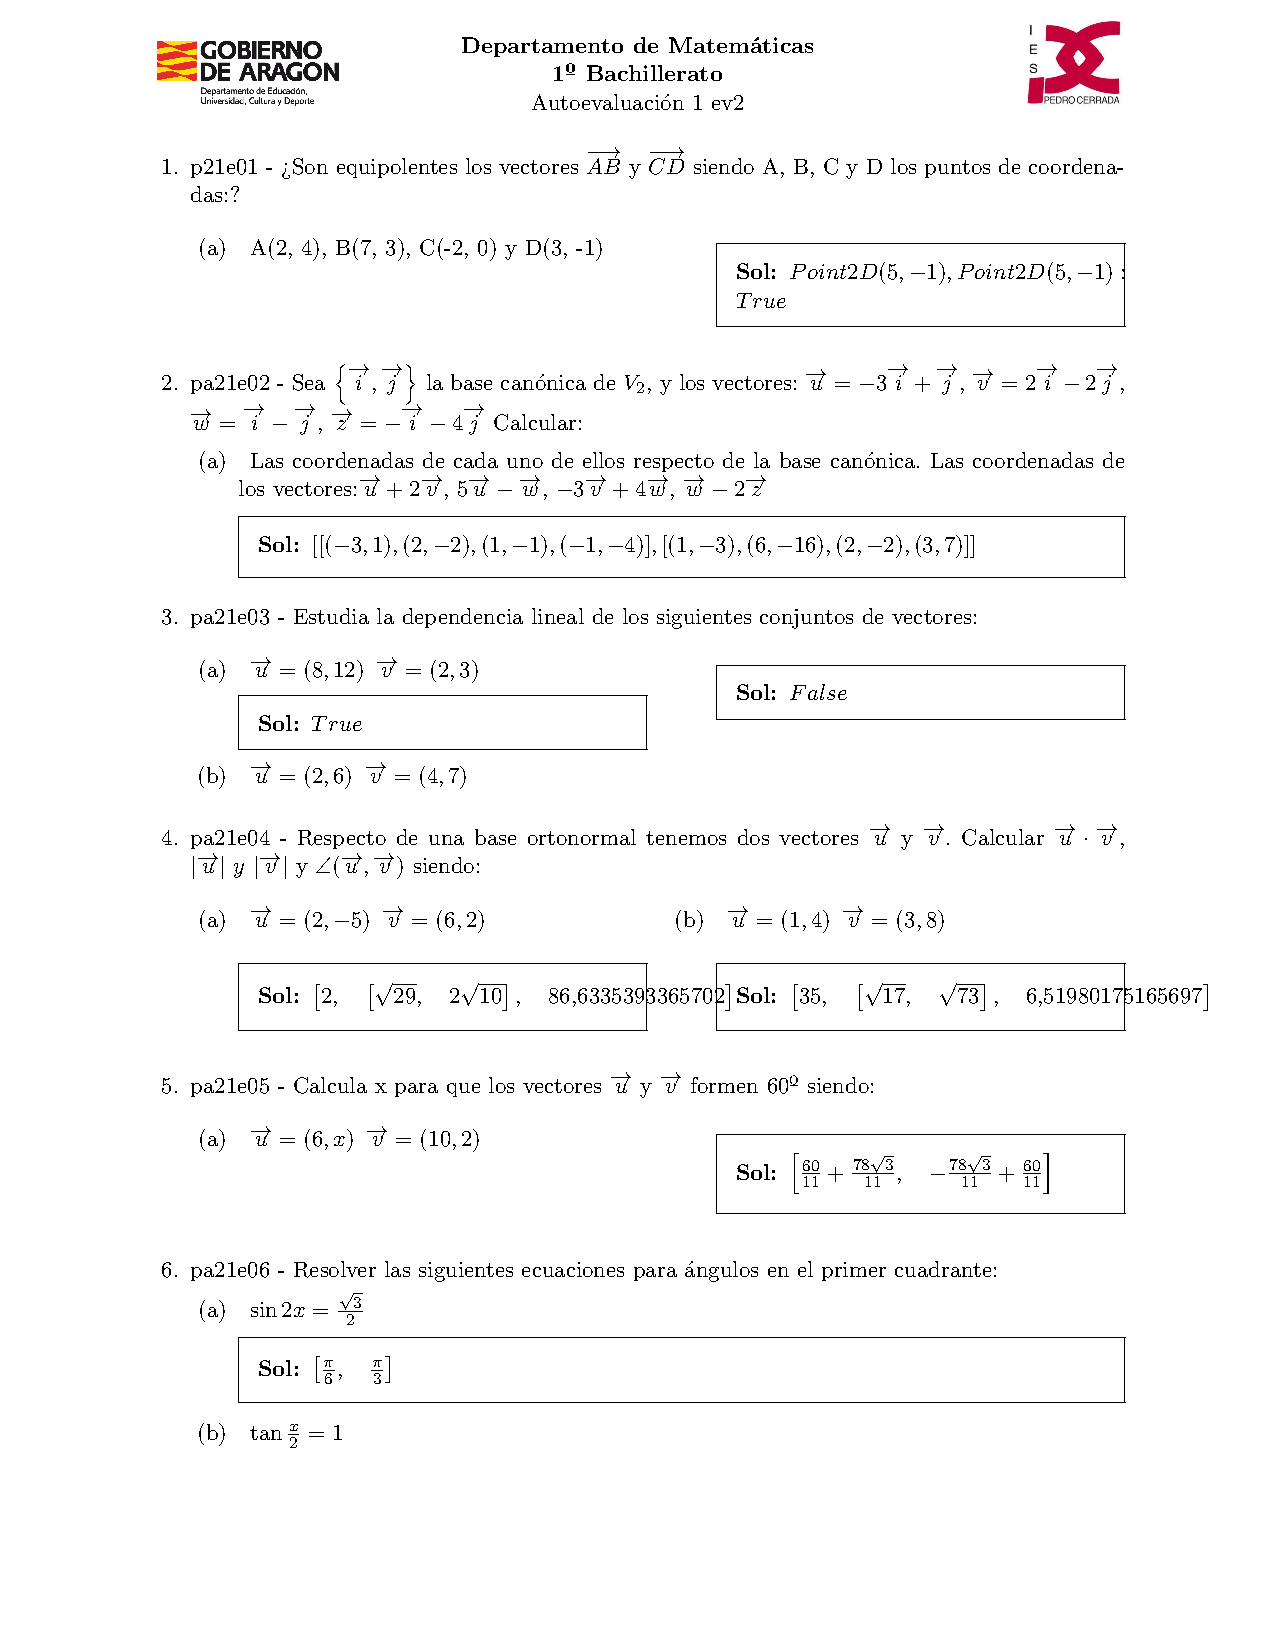
\includepdf[pages=-, scale=0.9]{2_geometria/autoev21.pdf}
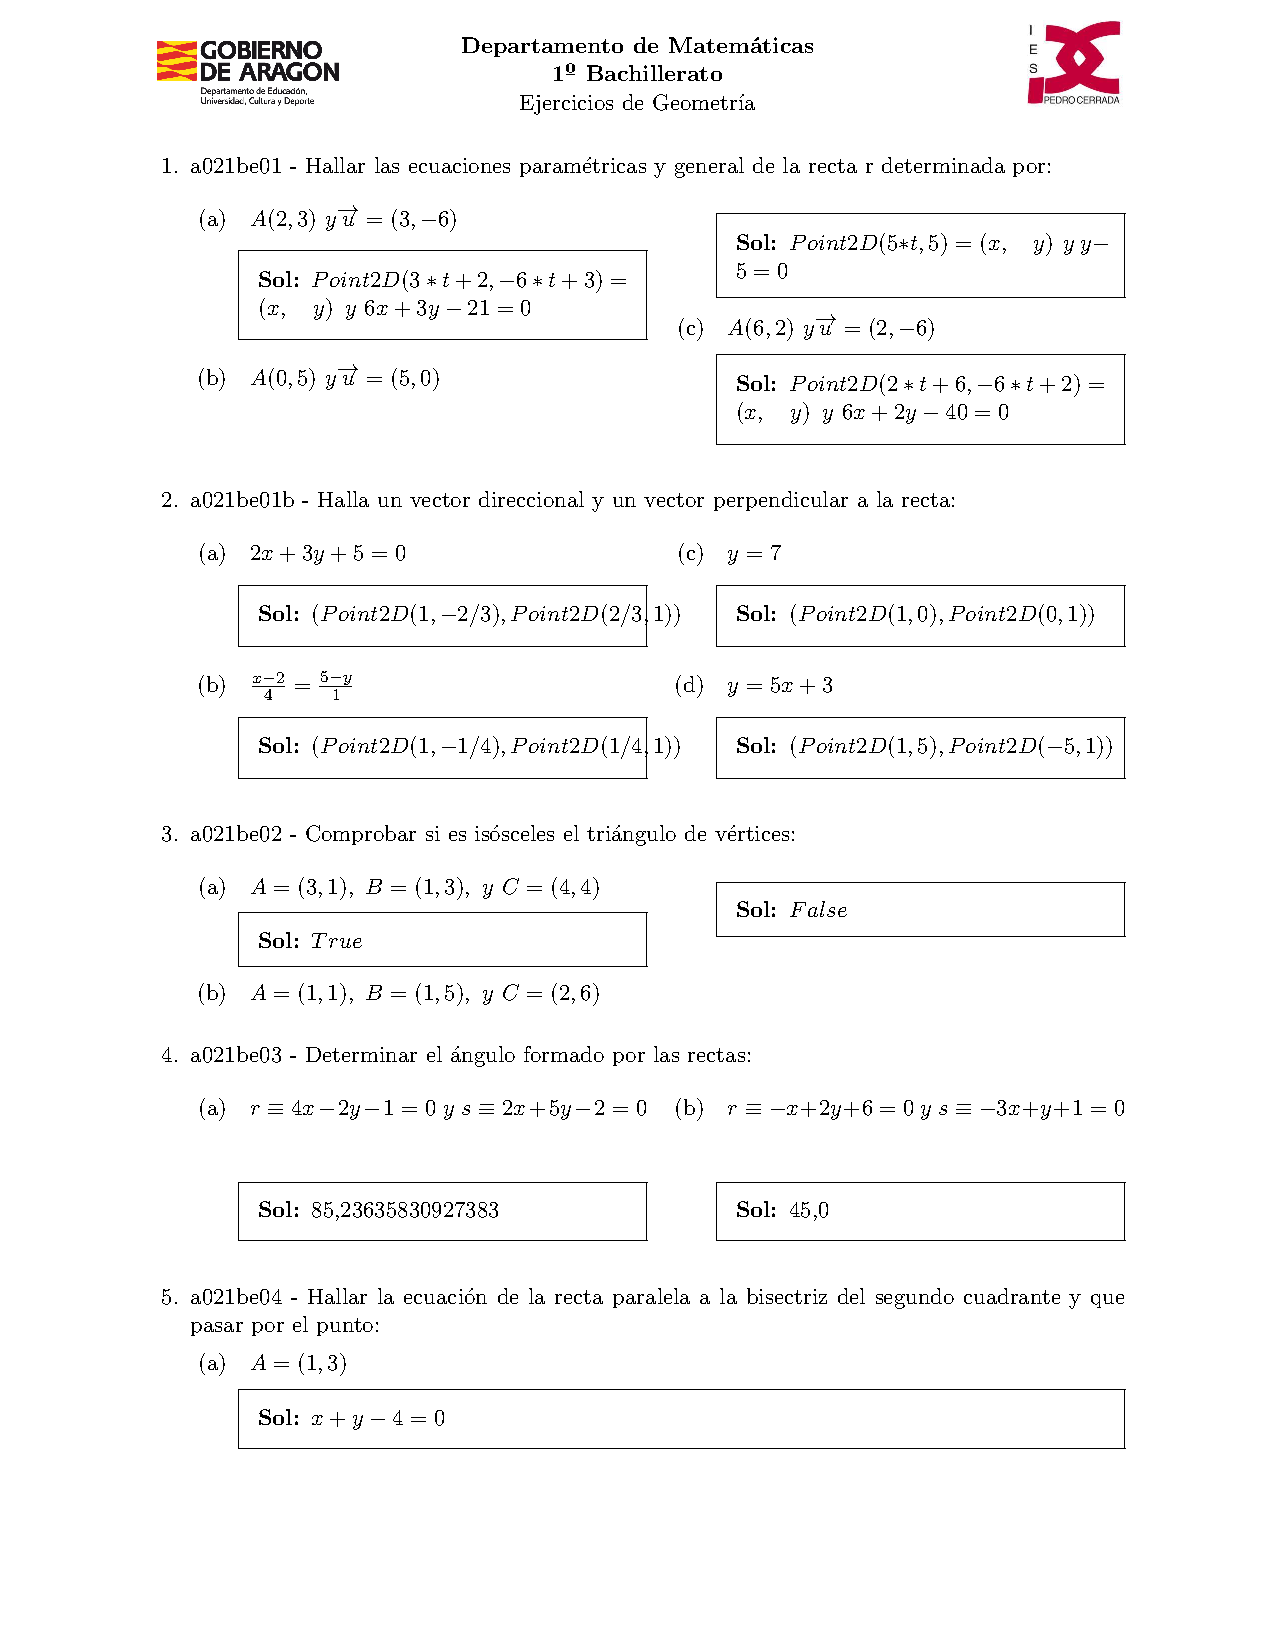
\includepdf[pages=-, scale=0.9]{2_geometria/autoevaluacion21b.pdf}
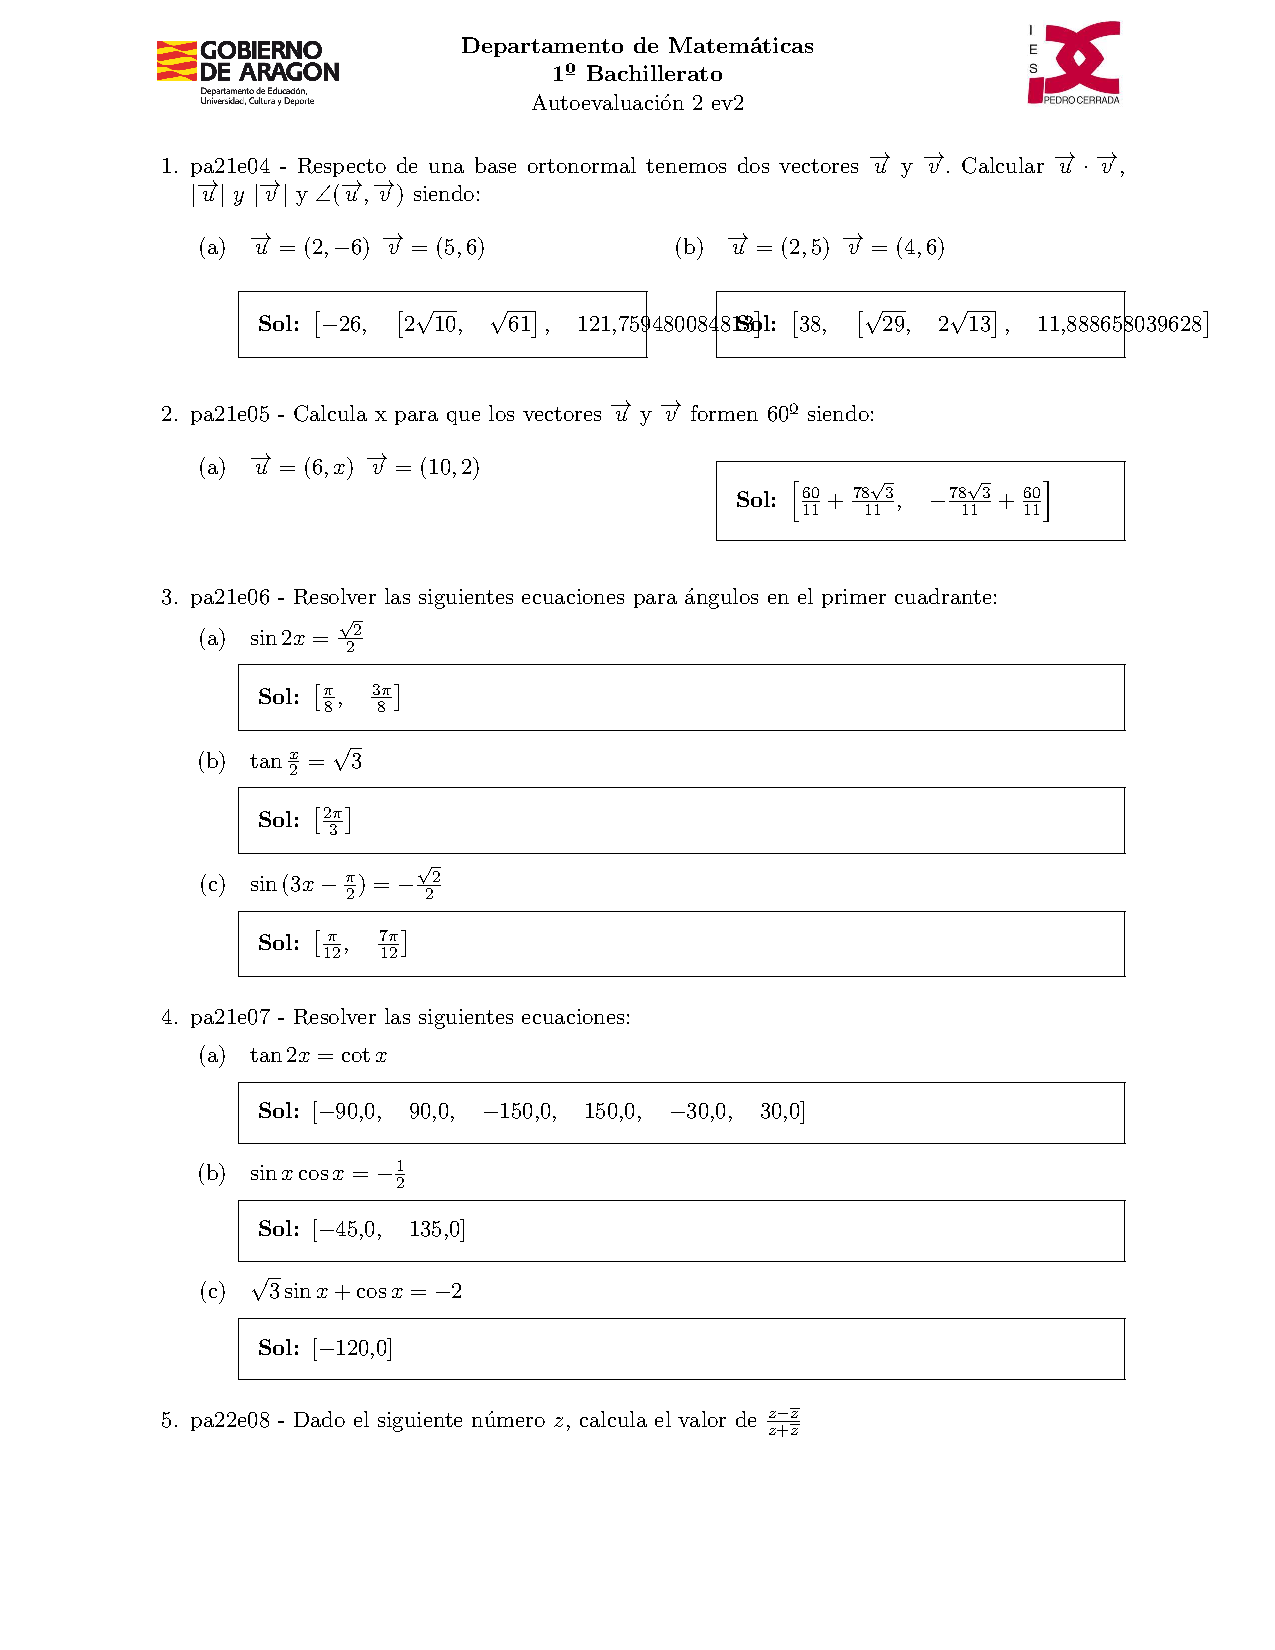
\includepdf[pages=-, scale=0.9]{2_geometria/autoev22.pdf}


\chapter{Estadística}

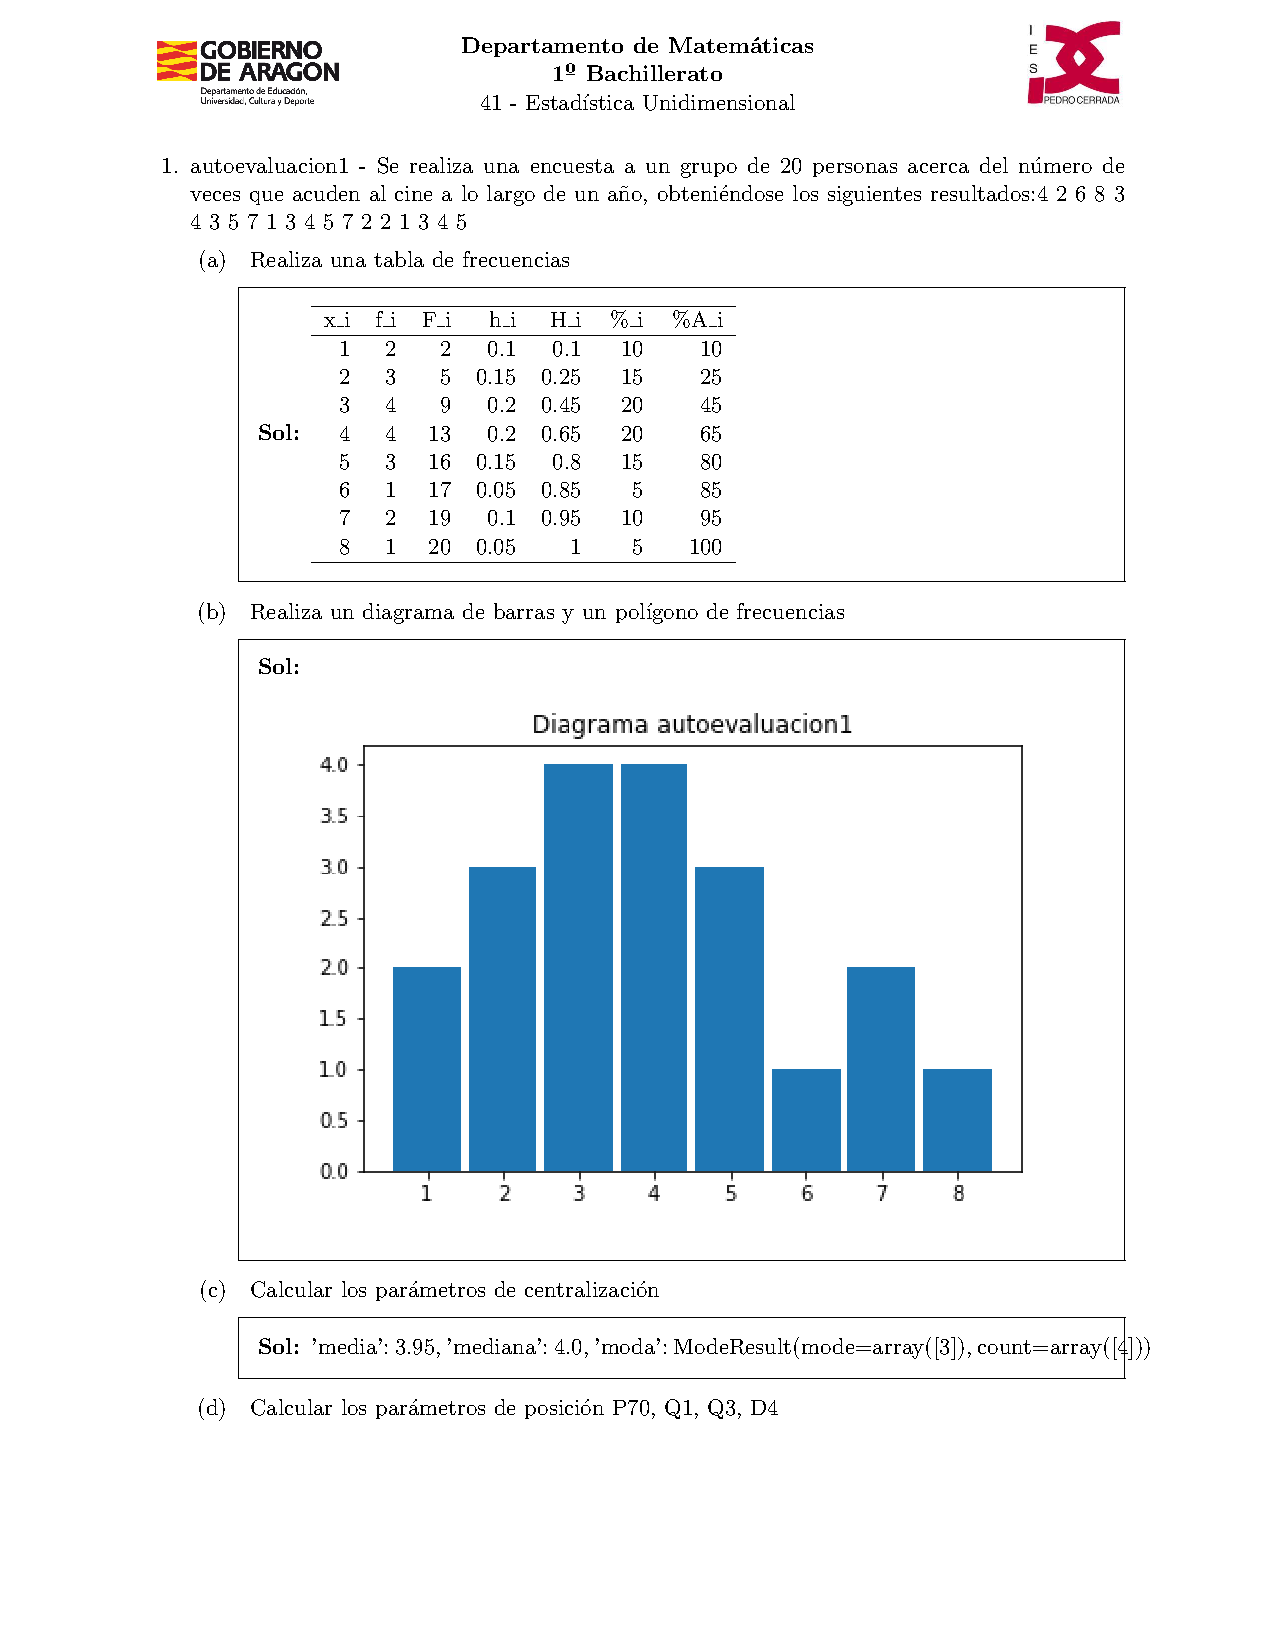
\includepdf[pages=-, scale=0.9]{3_estadistica/est1.pdf}
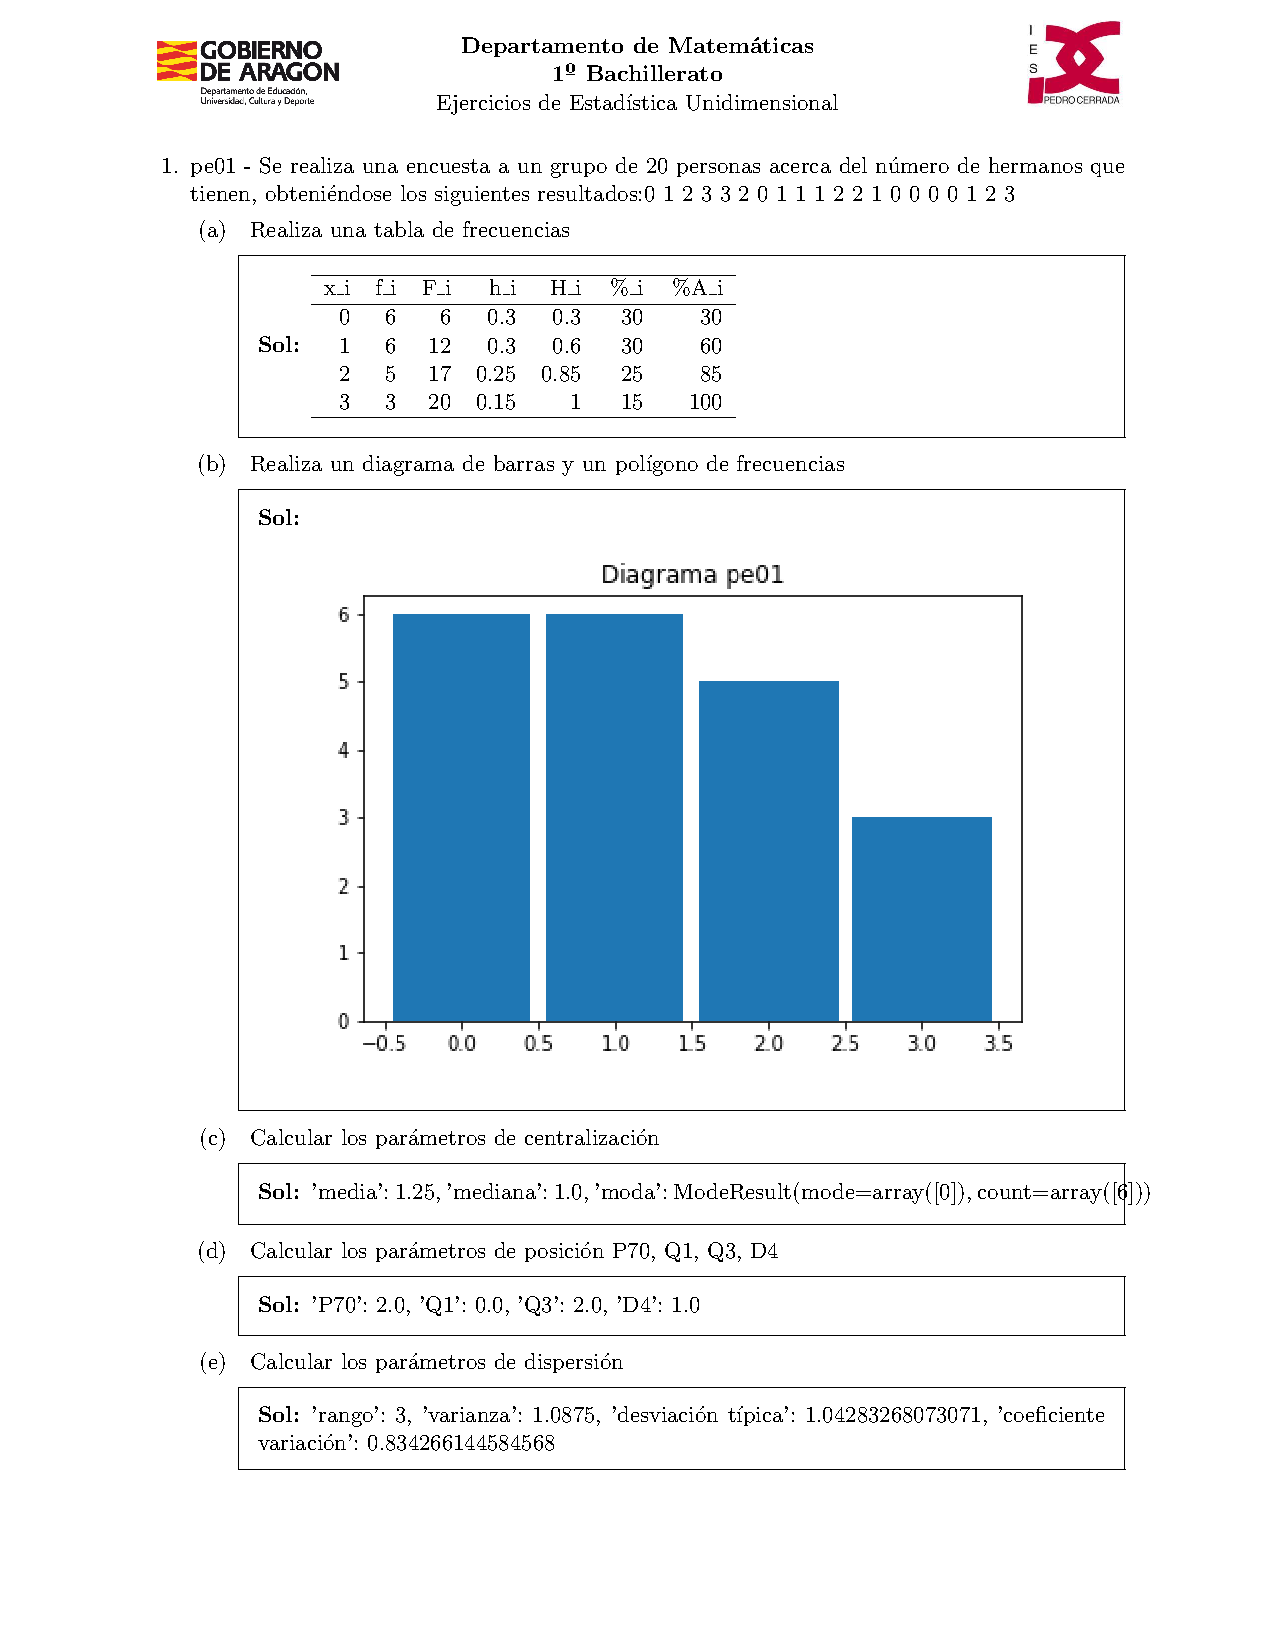
\includepdf[pages=-, scale=0.9]{3_estadistica/est_ejercicio_unidimensional.pdf}
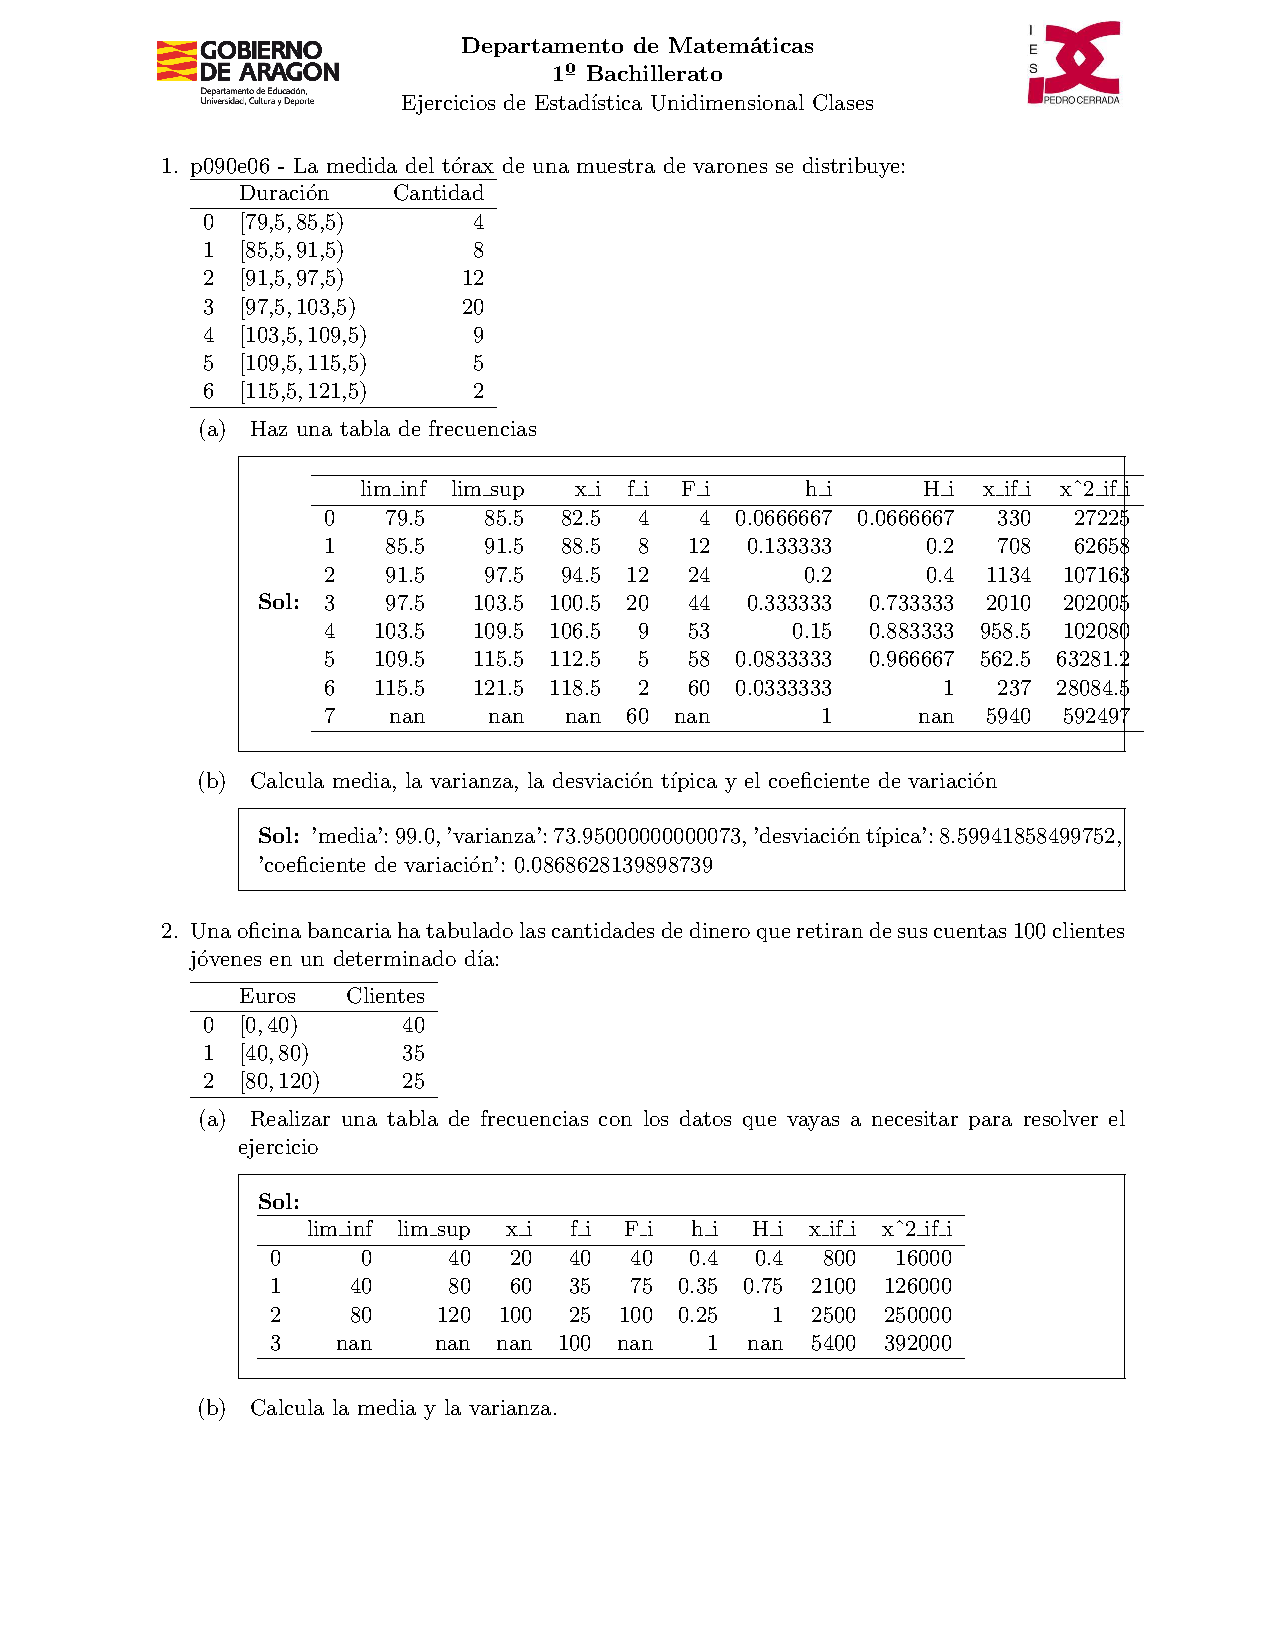
\includepdf[pages=-, scale=0.9]{3_estadistica/est_ejercicios_unidimensional_2.pdf}
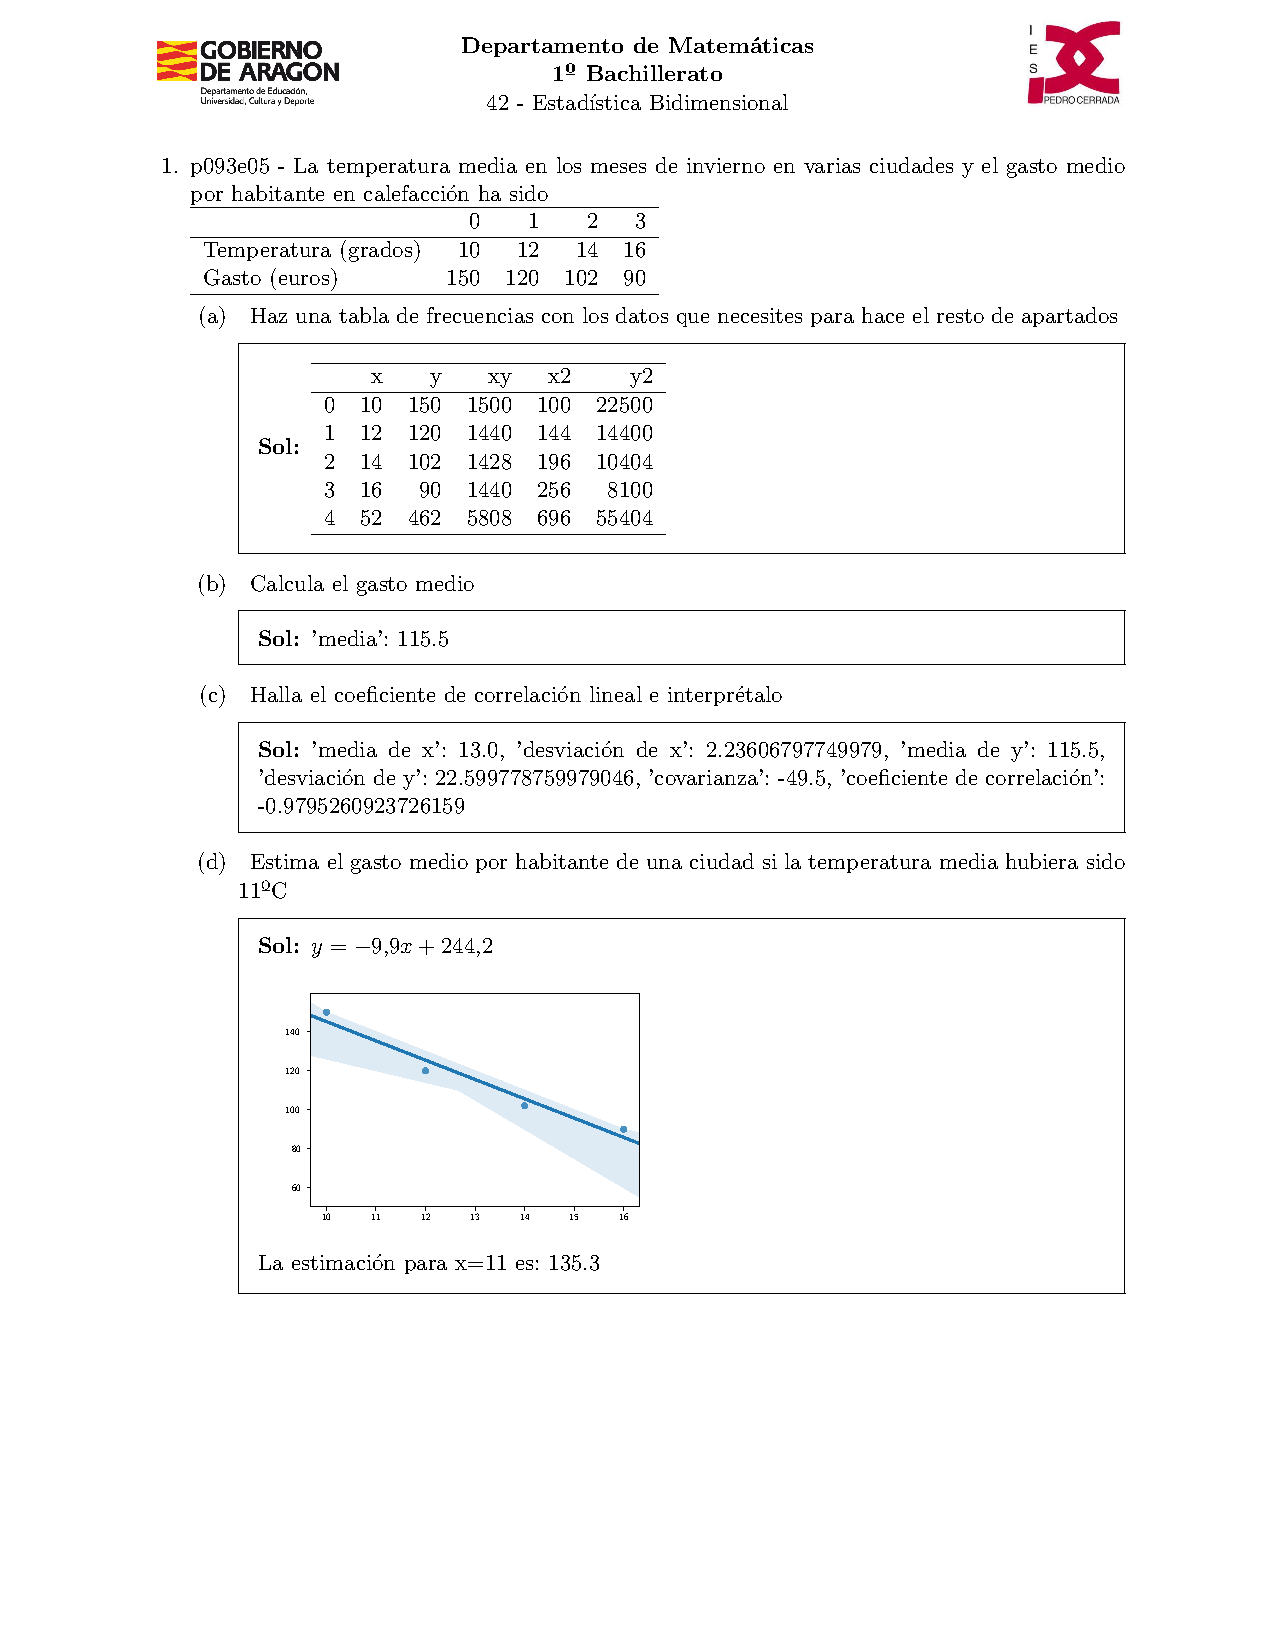
\includepdf[pages=-, scale=0.9]{3_estadistica/est2.pdf}
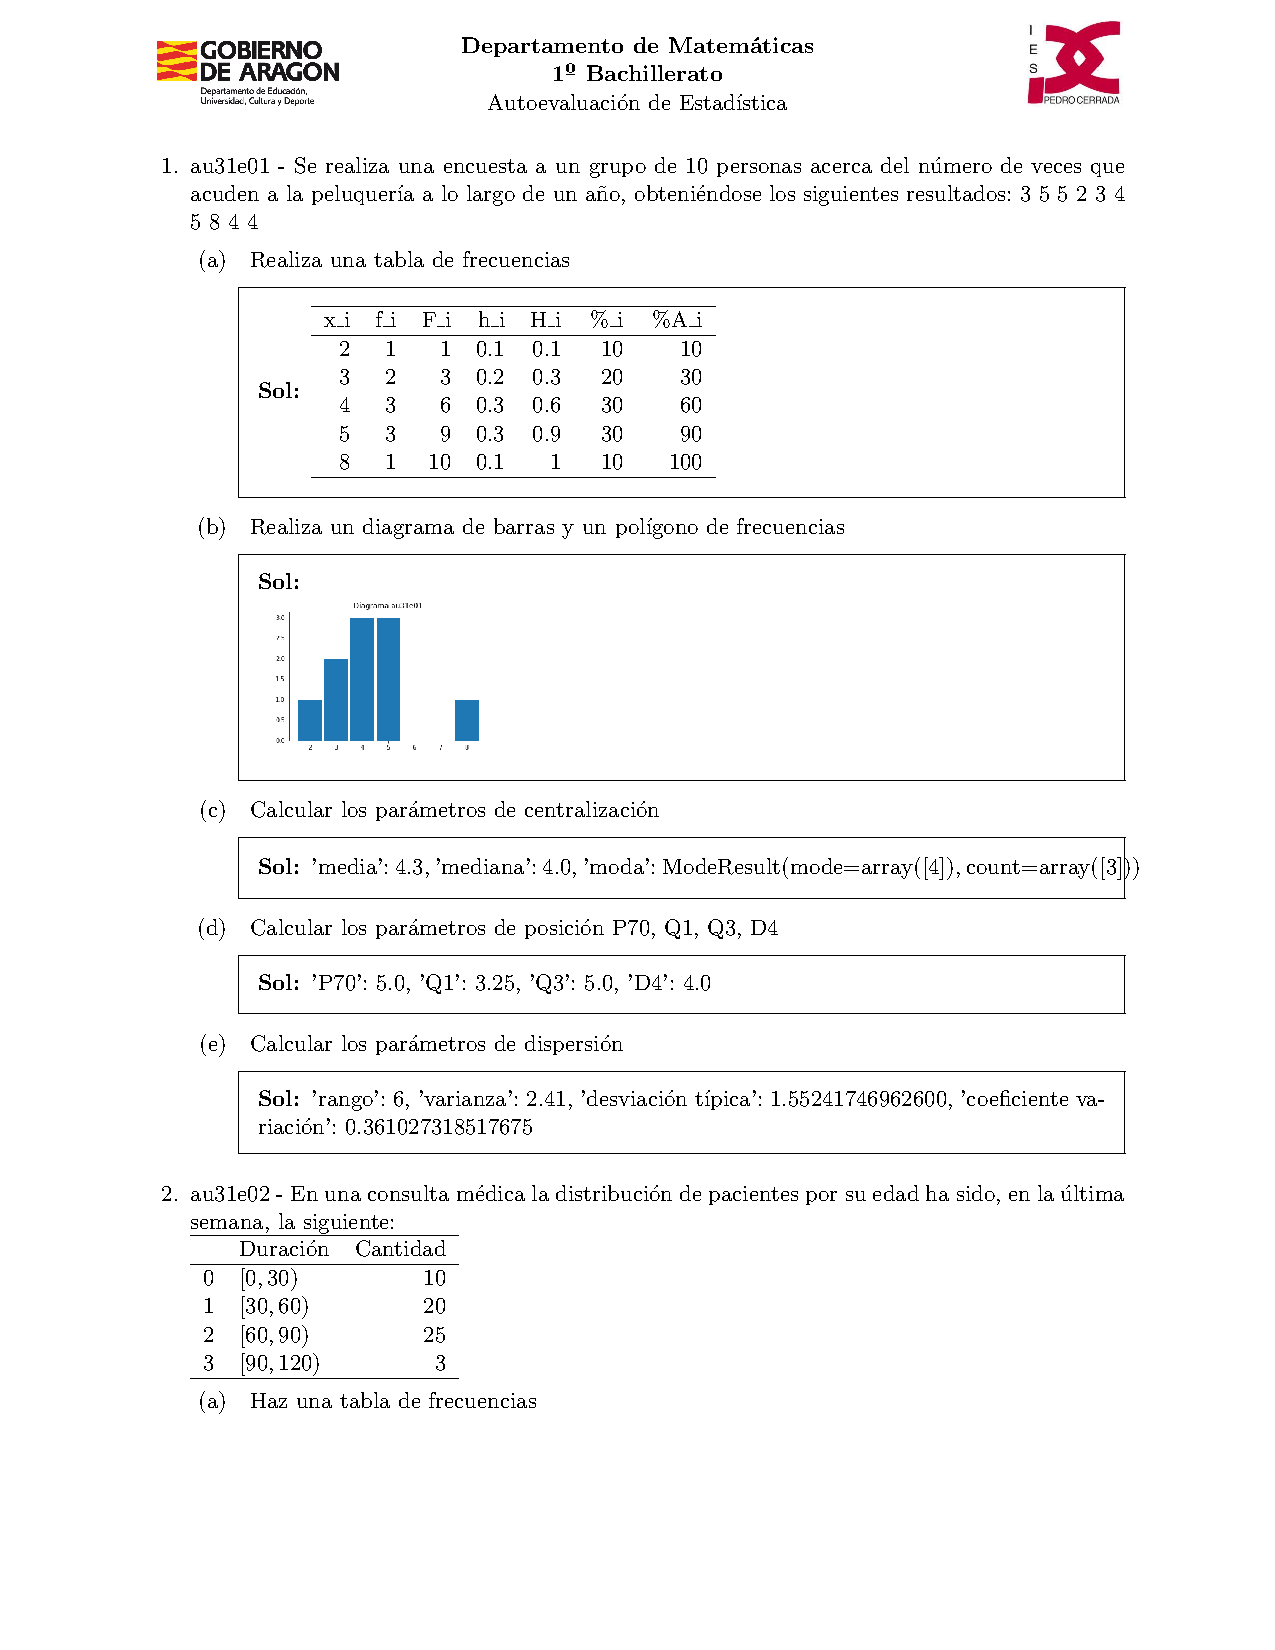
\includepdf[pages=-, scale=0.9]{3_estadistica/autoev_est.pdf}
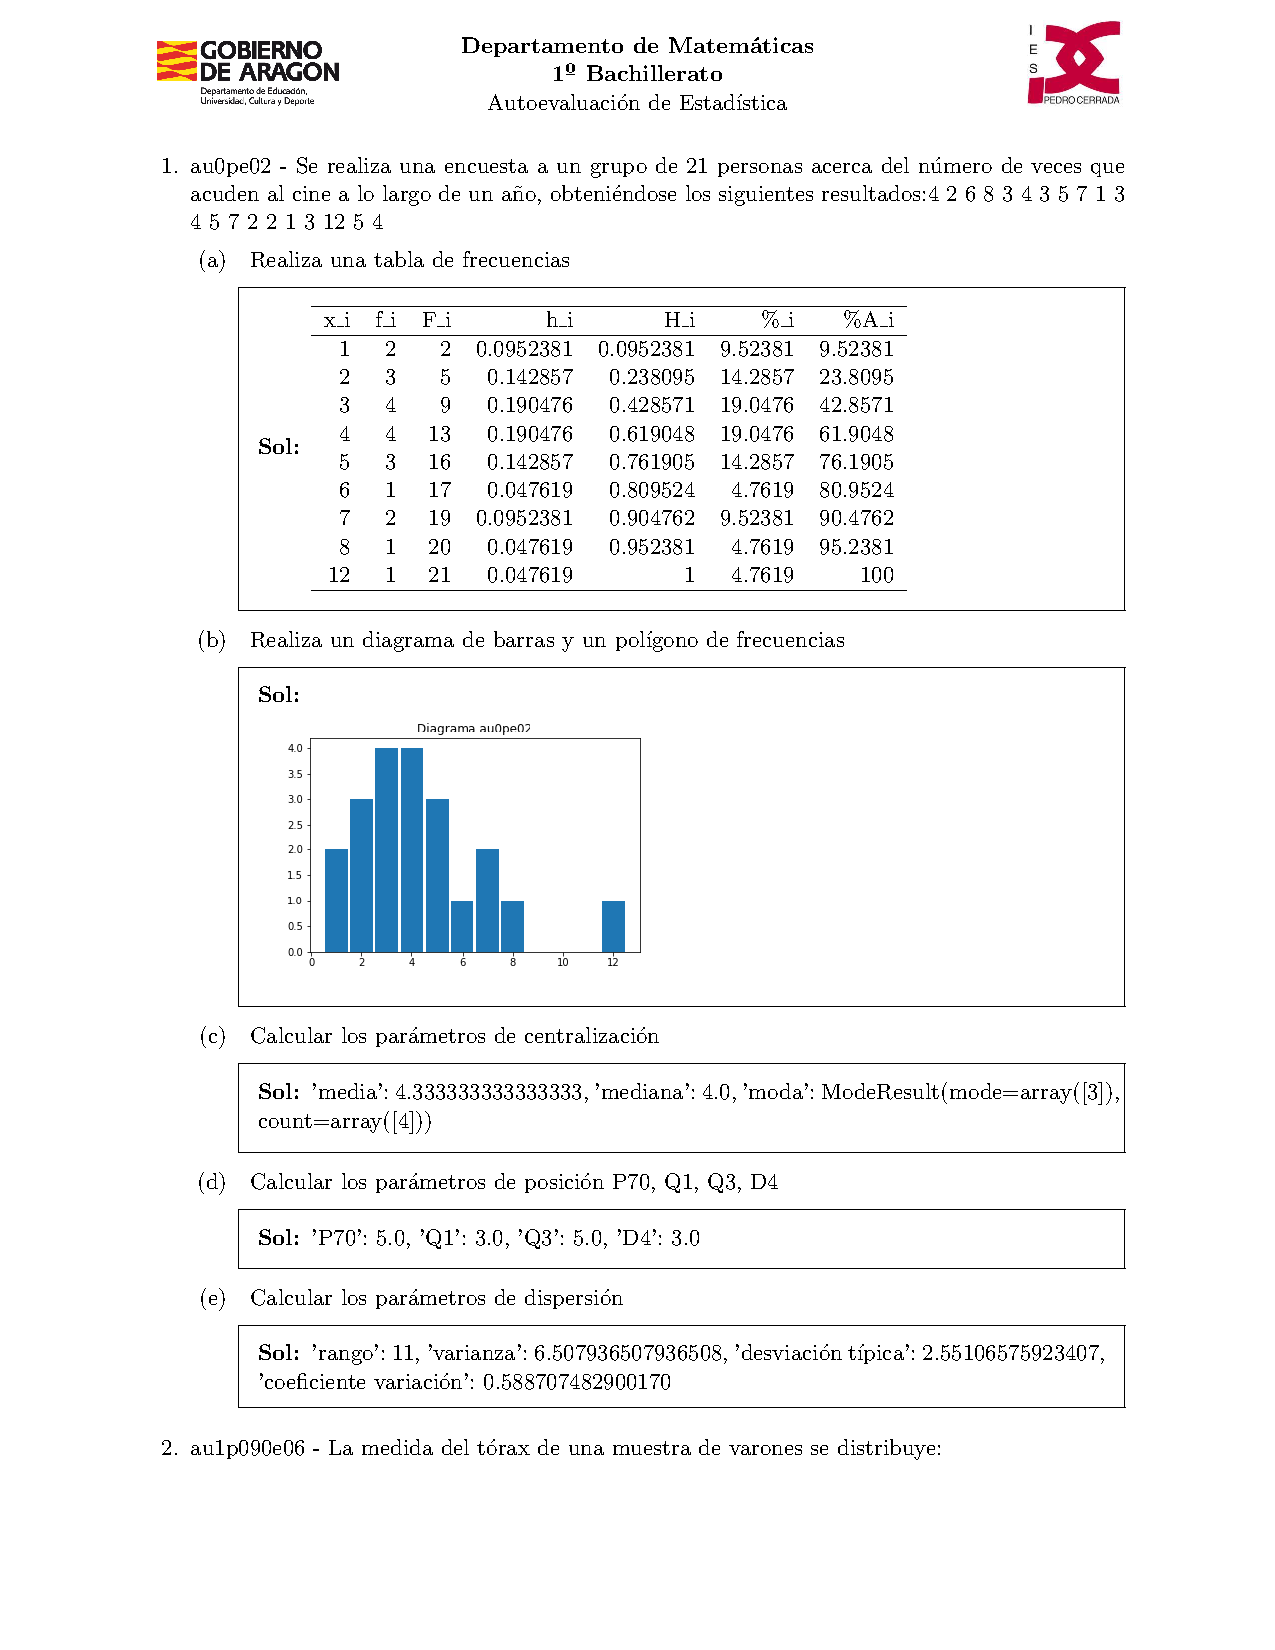
\includepdf[pages=-, scale=0.9]{3_estadistica/autoev2_est.pdf}
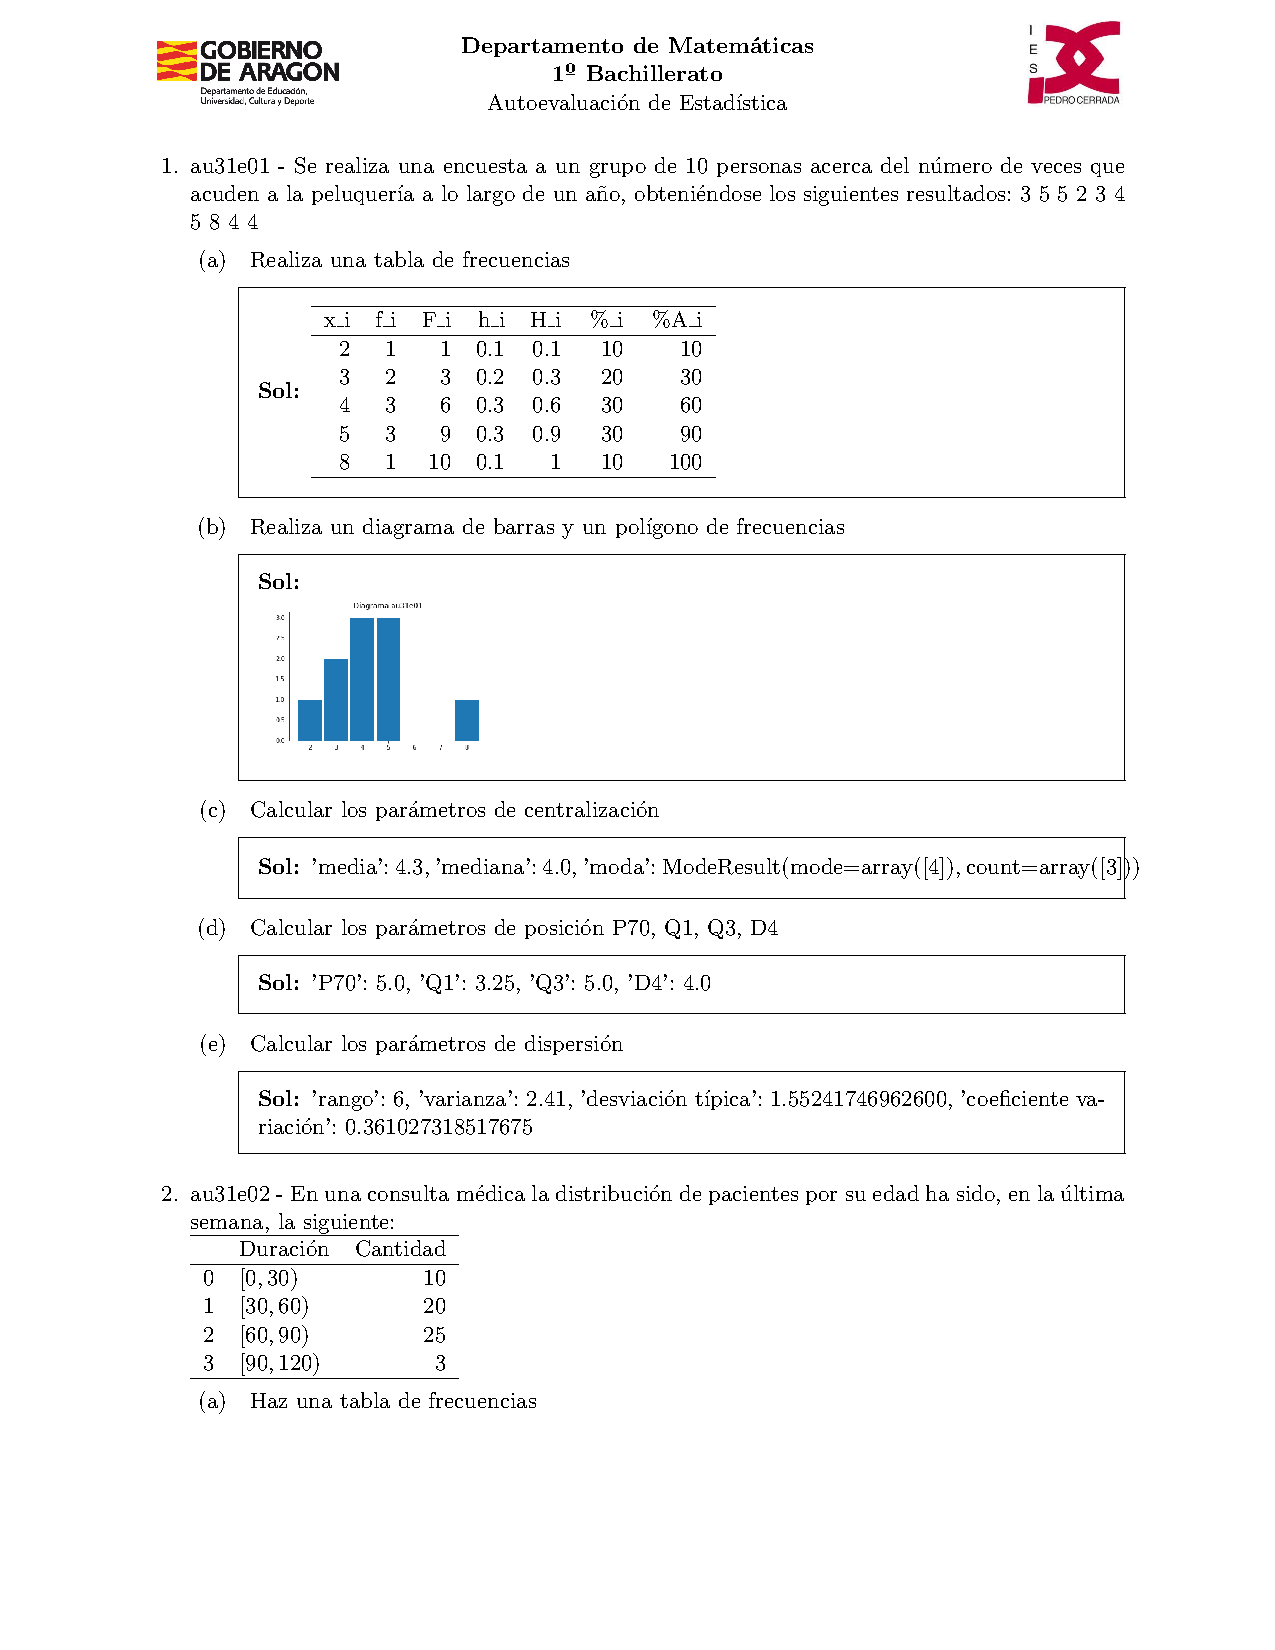
\includepdf[pages=-, scale=0.9]{3_estadistica/autoev_est.pdf}
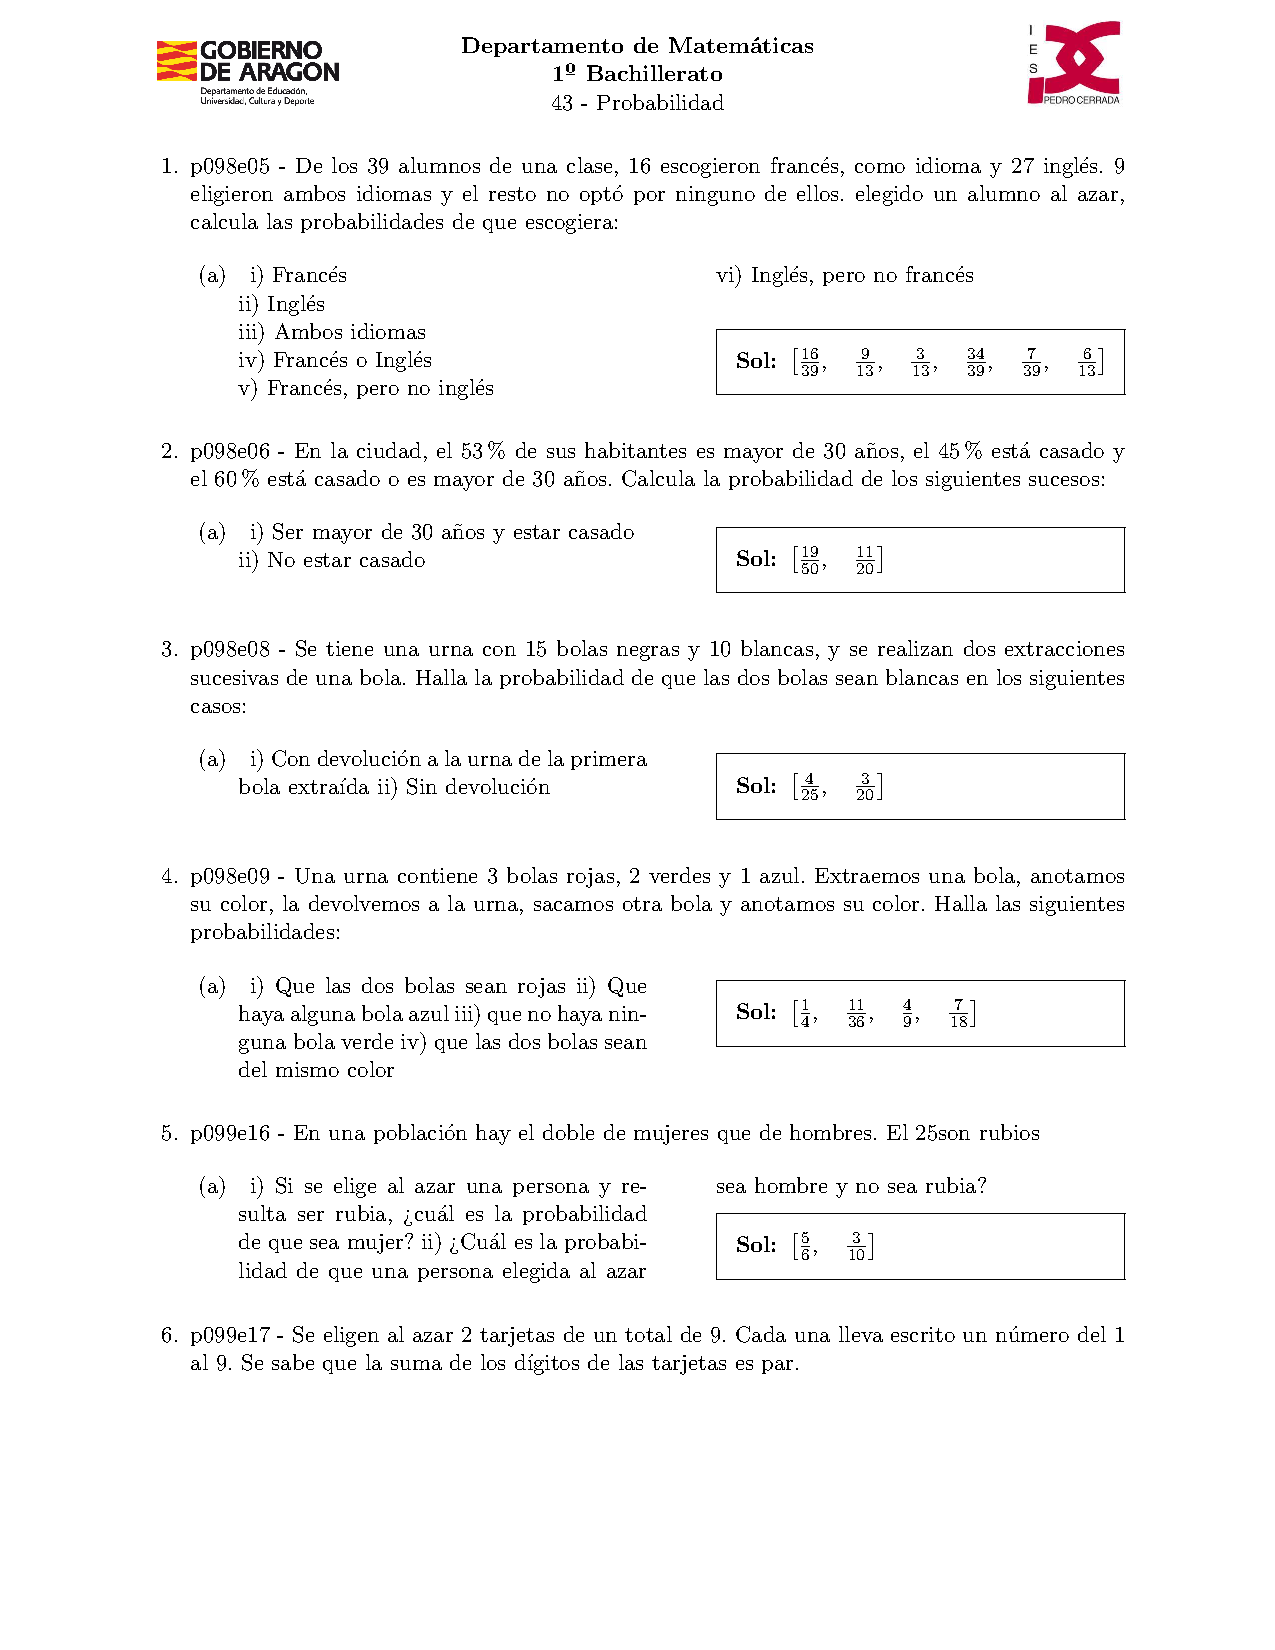
\includepdf[pages=-, scale=0.9]{3_estadistica/probab.pdf}
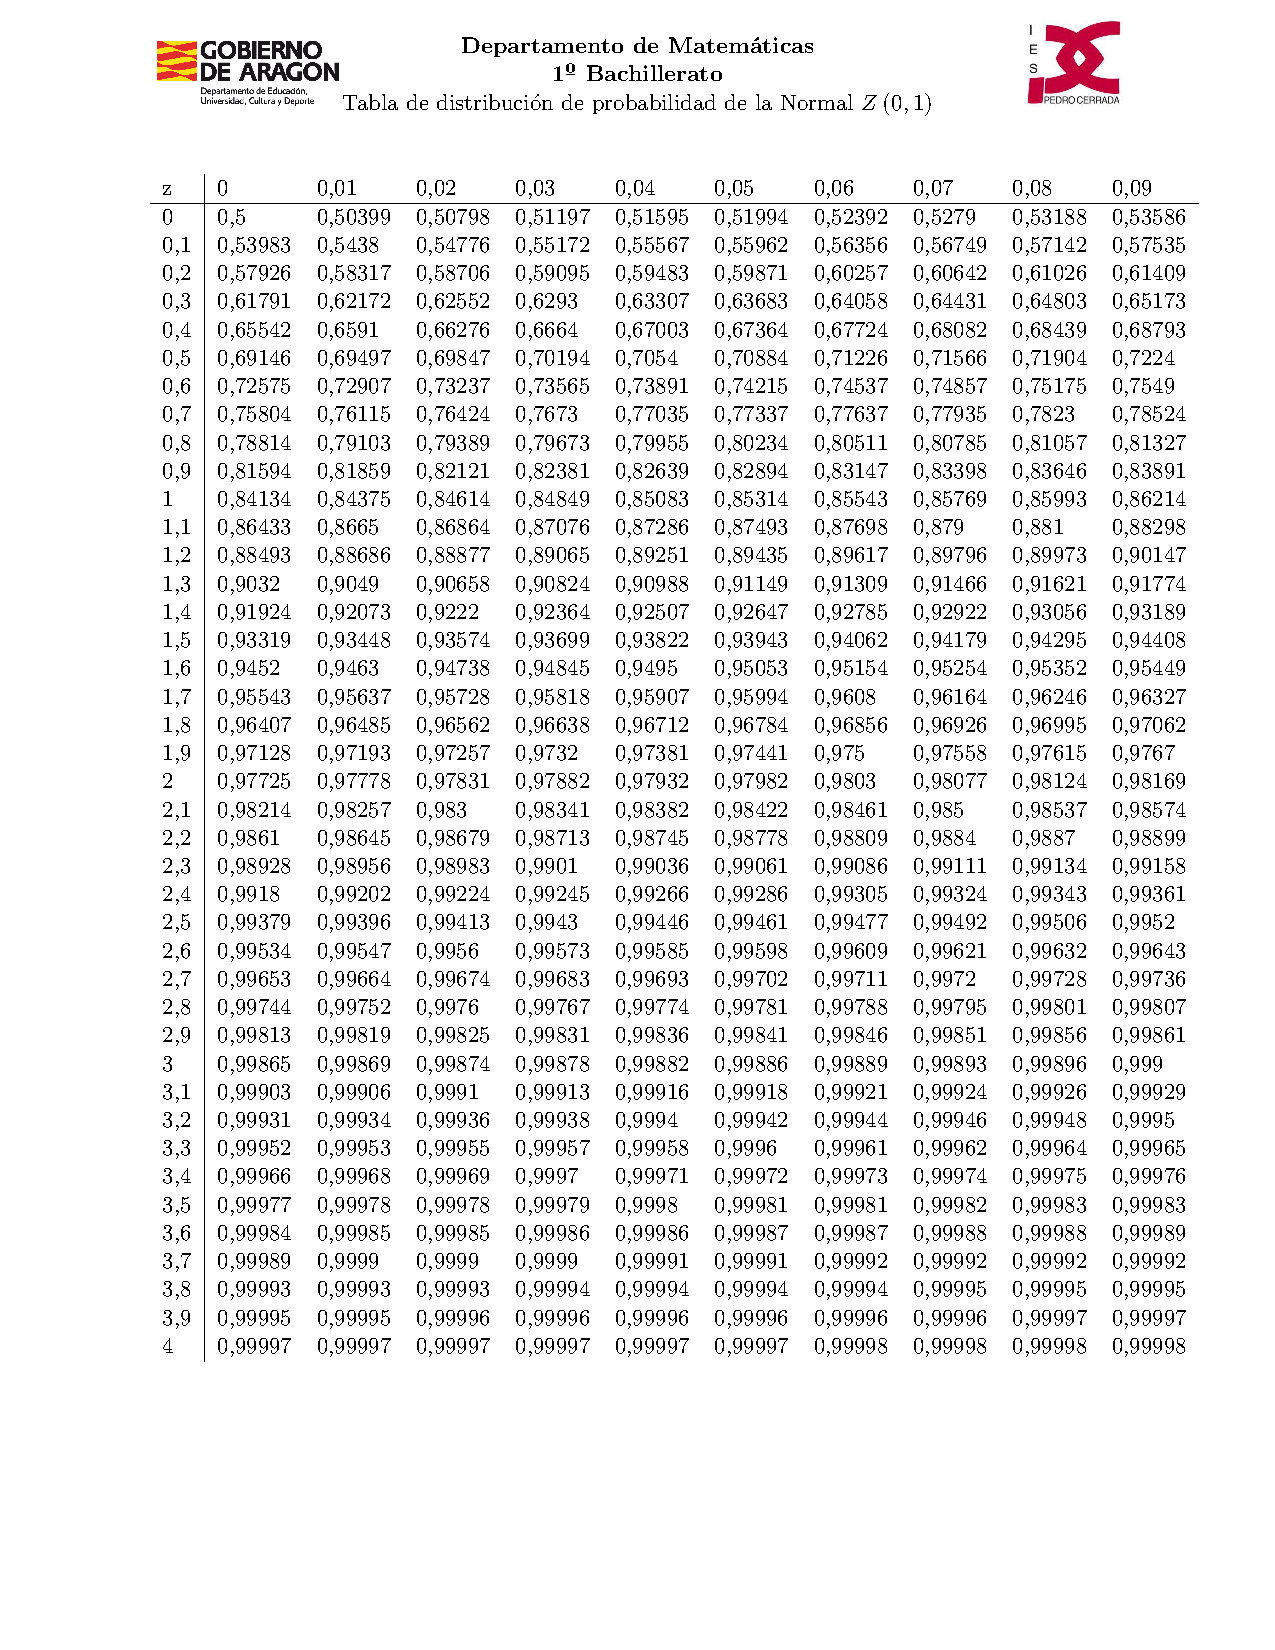
\includepdf[pages=-, scale=0.9]{3_estadistica/var_ale_tabla_normal.pdf}
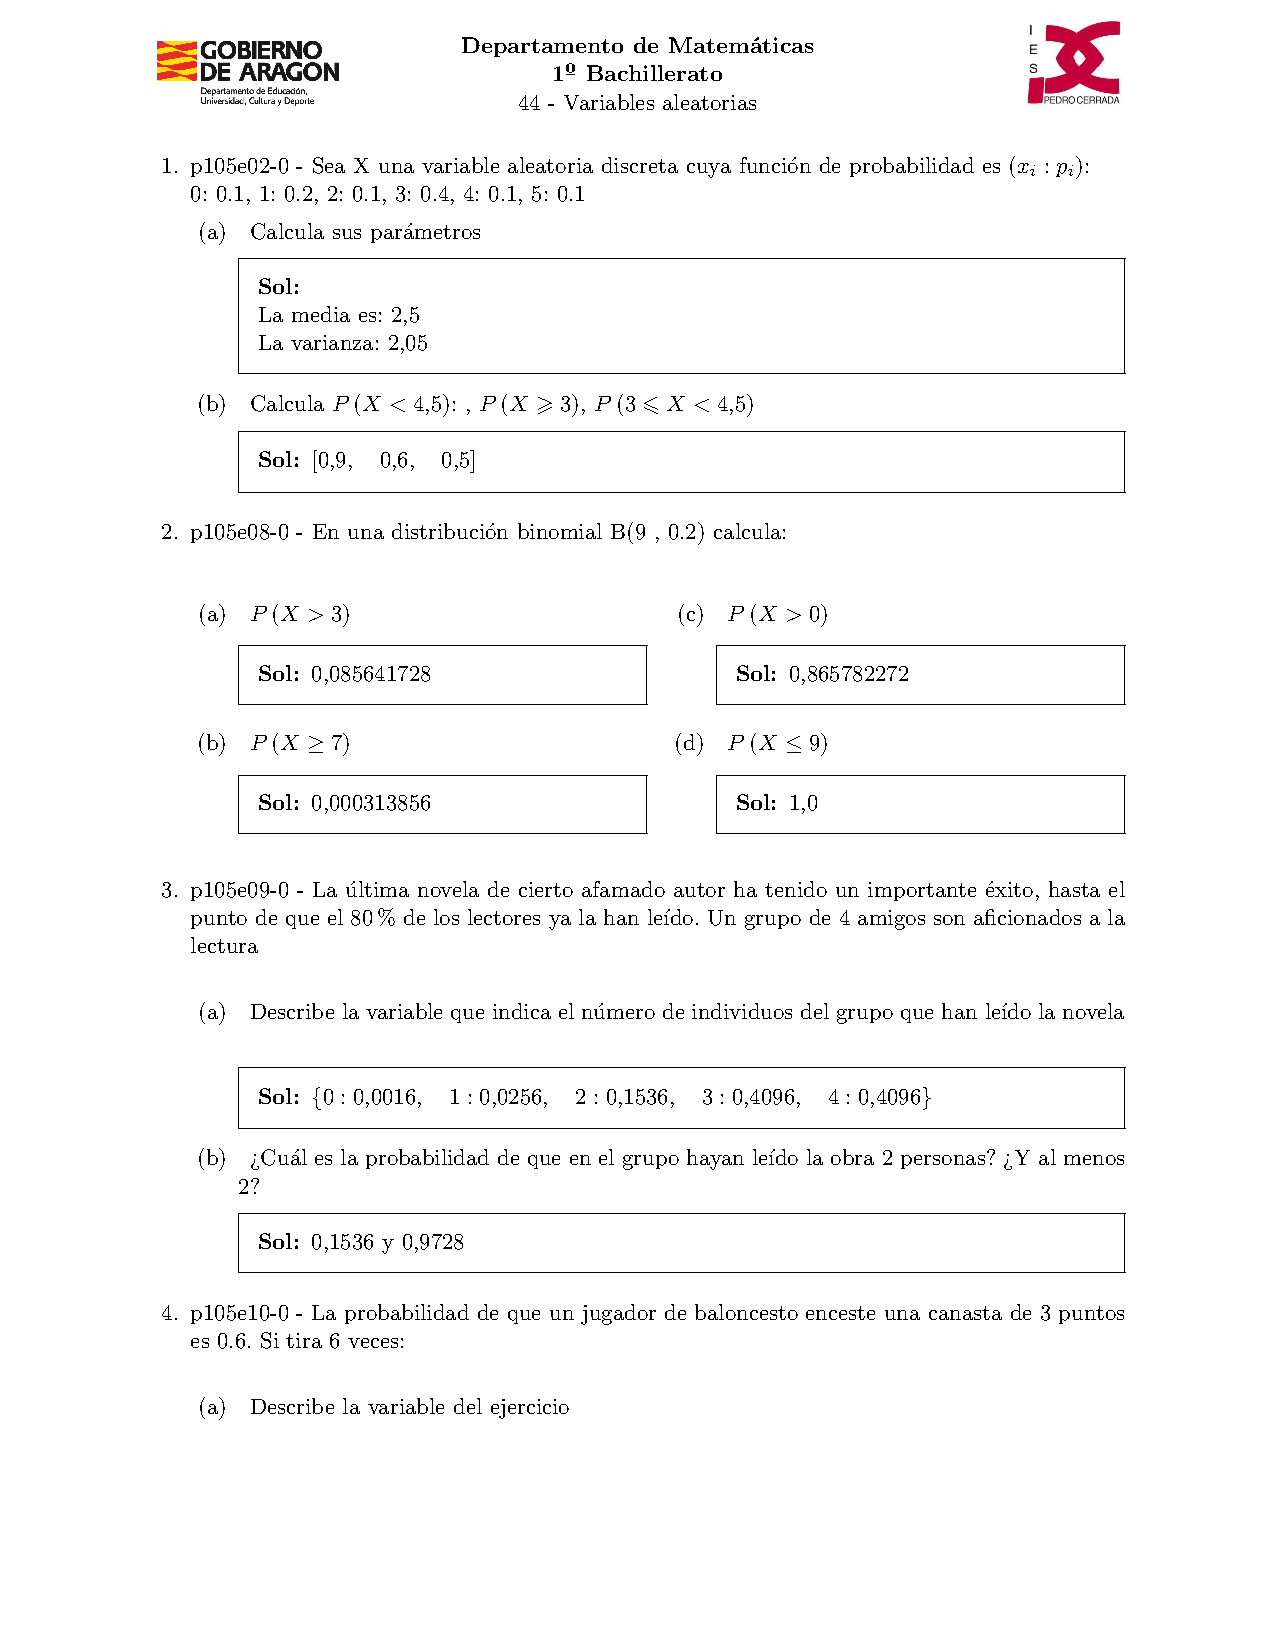
\includepdf[pages=-, scale=0.9]{3_estadistica/var_ale.pdf}




%\input{probabilidad/probabilidad}
%\input{probabilidad/distribuciones}

\chapter{Análisis}
%\input{miscelanea/puntos_triangulo}
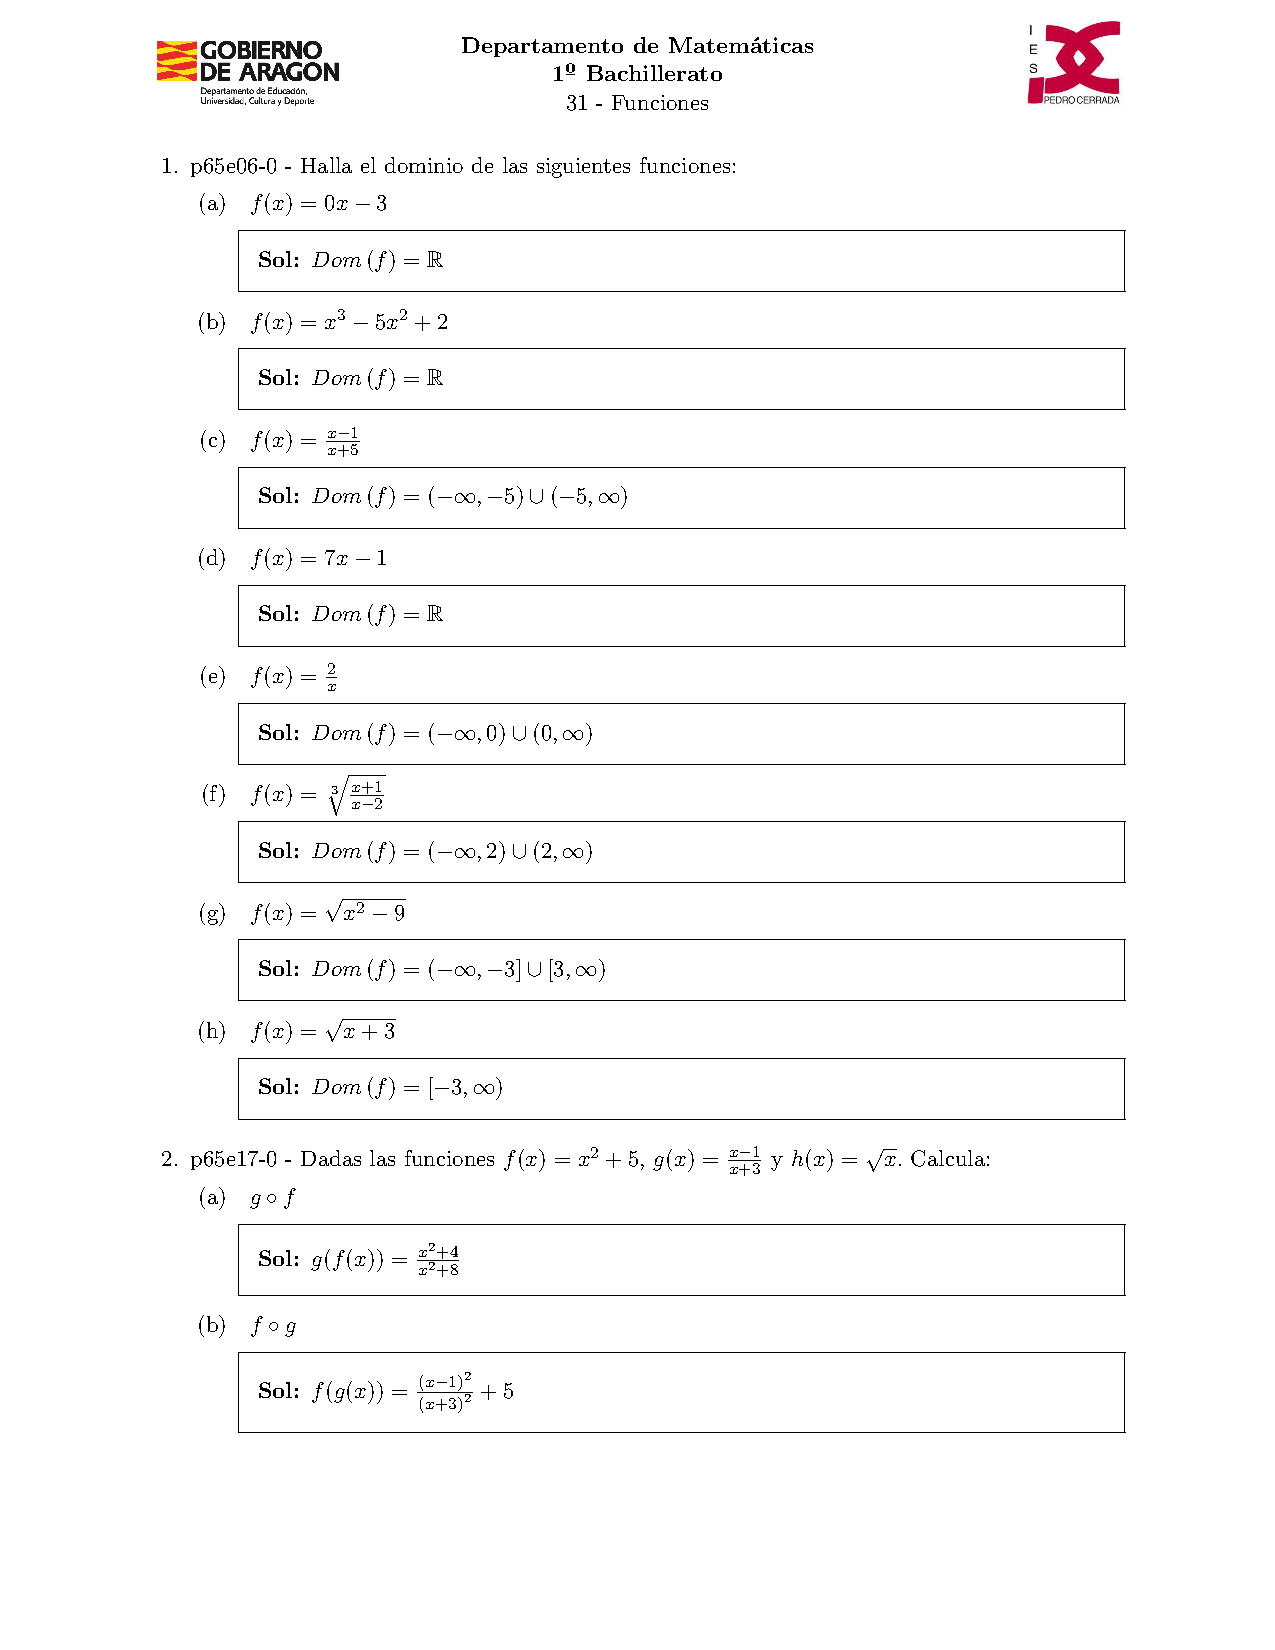
\includepdf[pages=-, scale=0.9]{4_analisis/func.pdf}
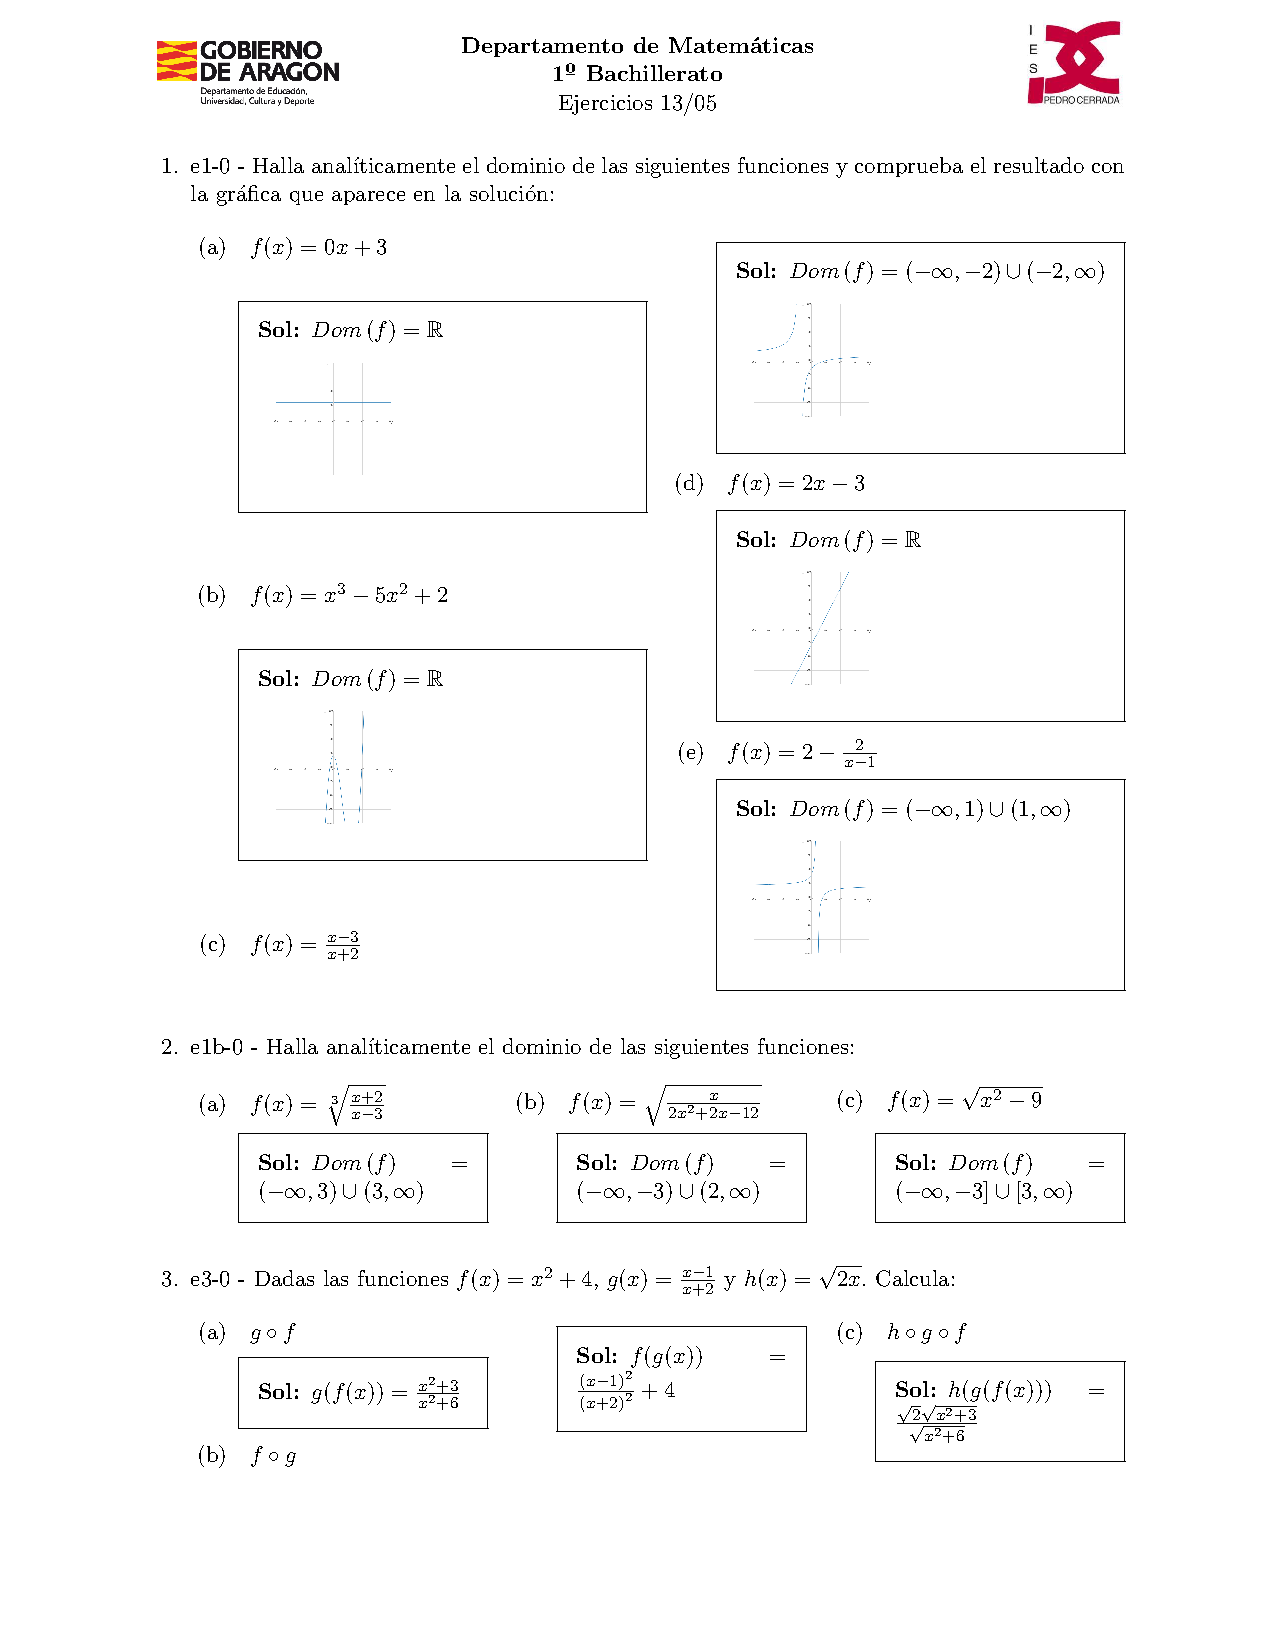
\includepdf[pages=-, scale=0.9]{4_analisis/autoev1305.pdf}
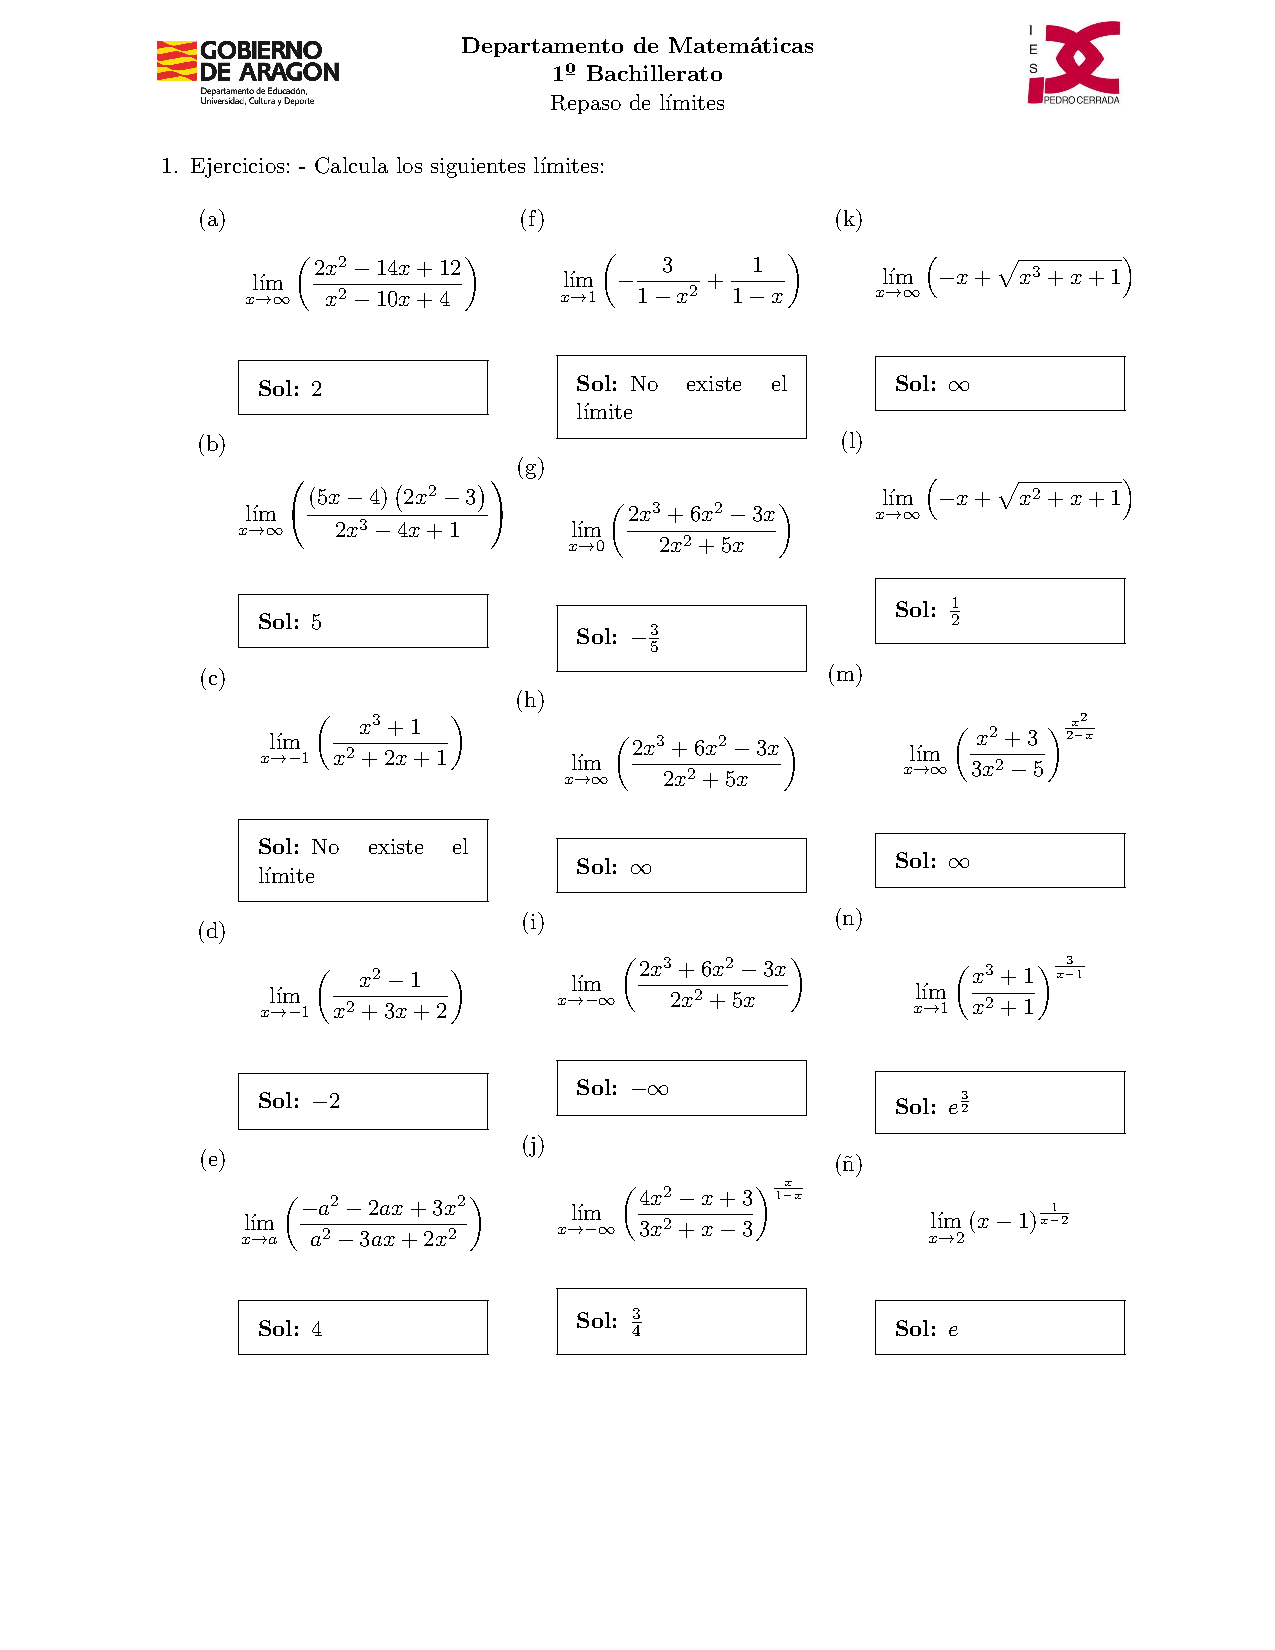
\includepdf[pages=-, scale=0.9]{4_analisis/rep_lim.pdf}
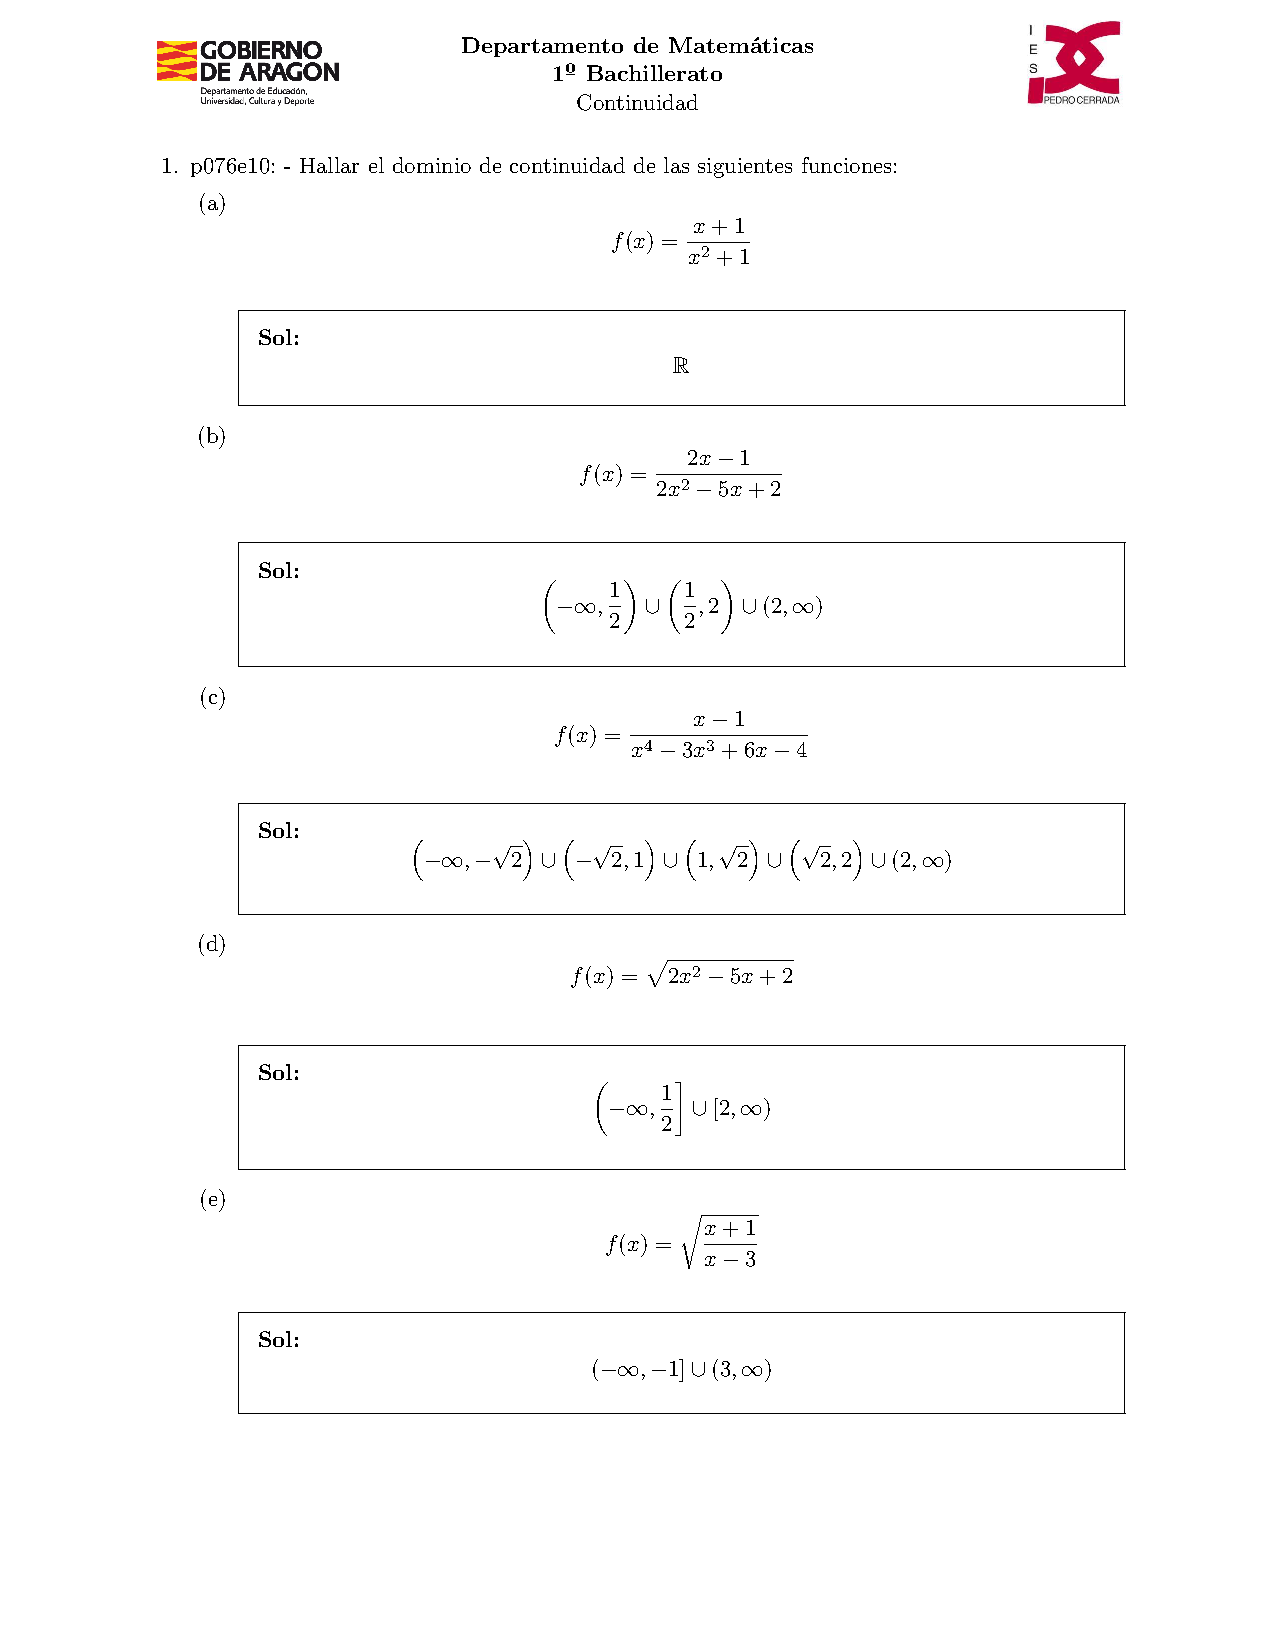
\includepdf[pages=-, scale=0.9]{4_analisis/continuidad.pdf}
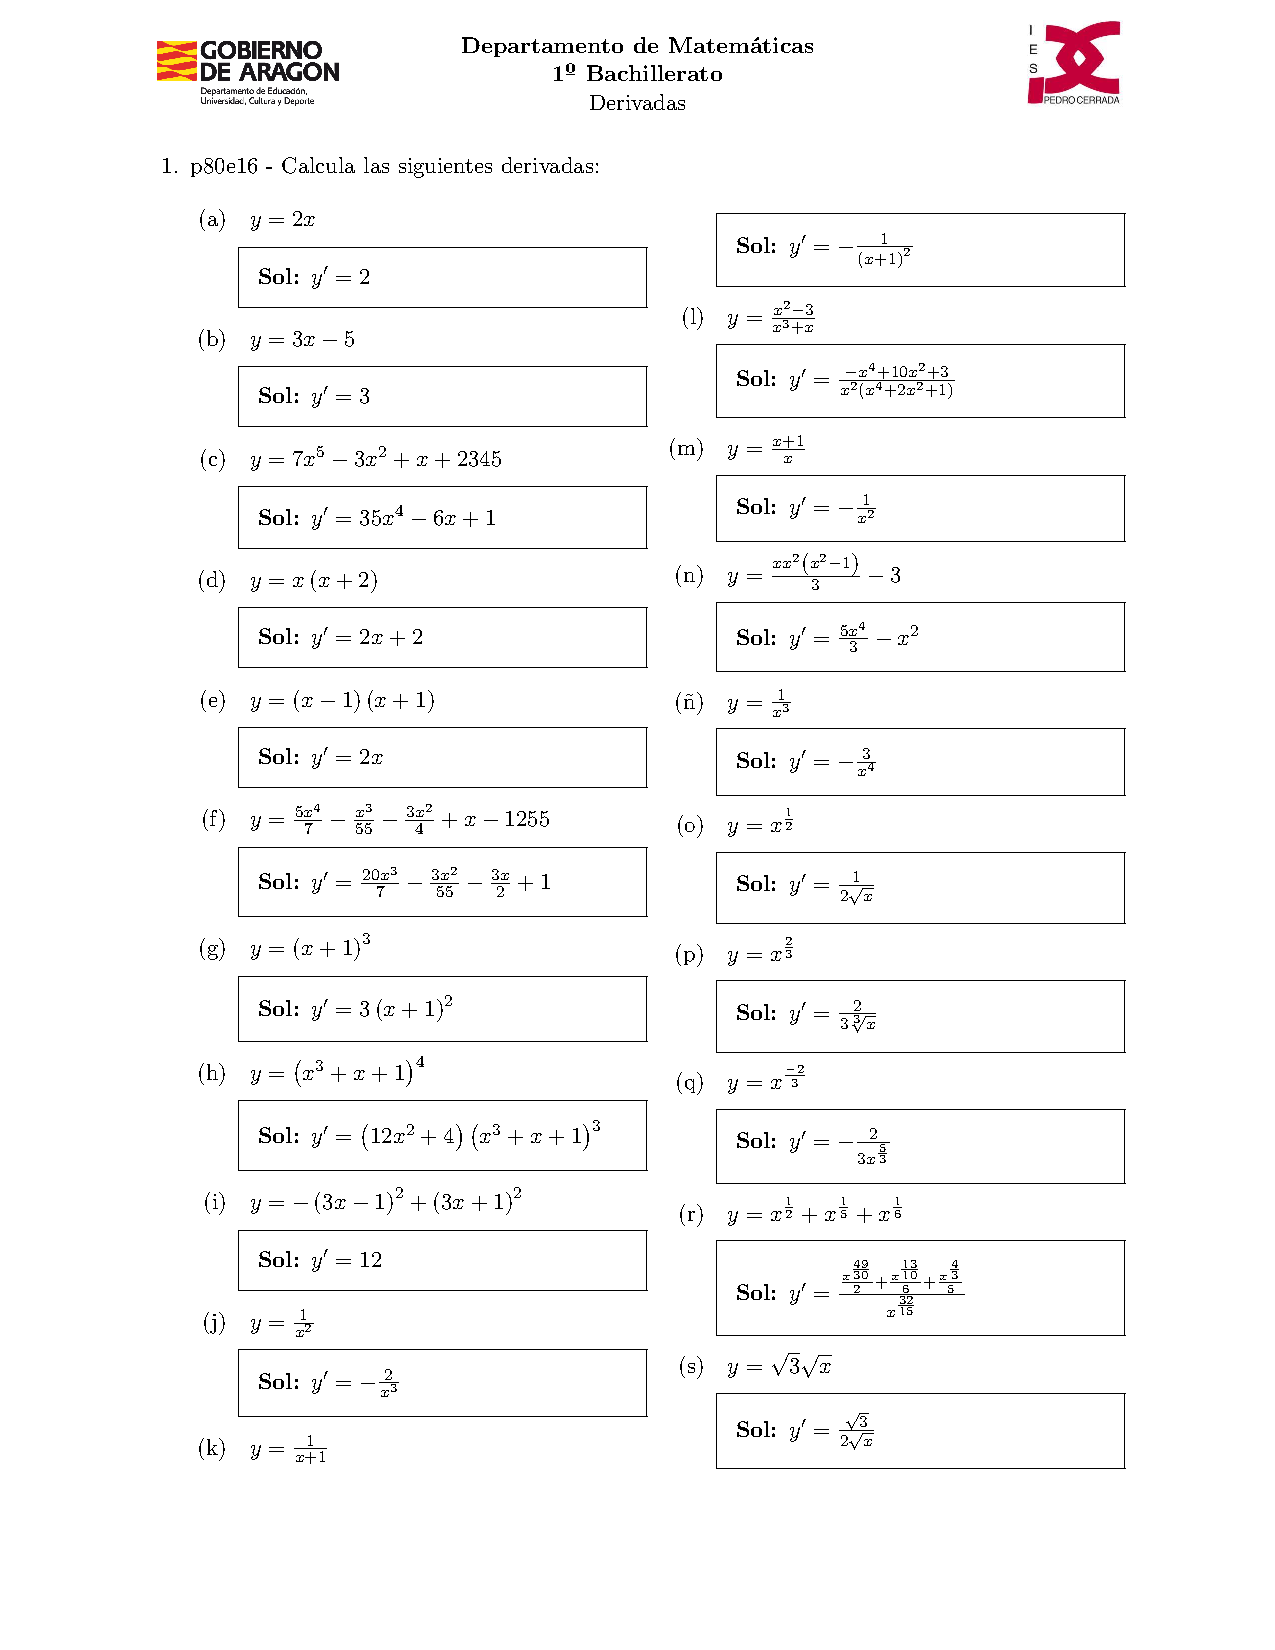
\includepdf[pages=-, scale=0.9]{4_analisis/deriv.pdf}
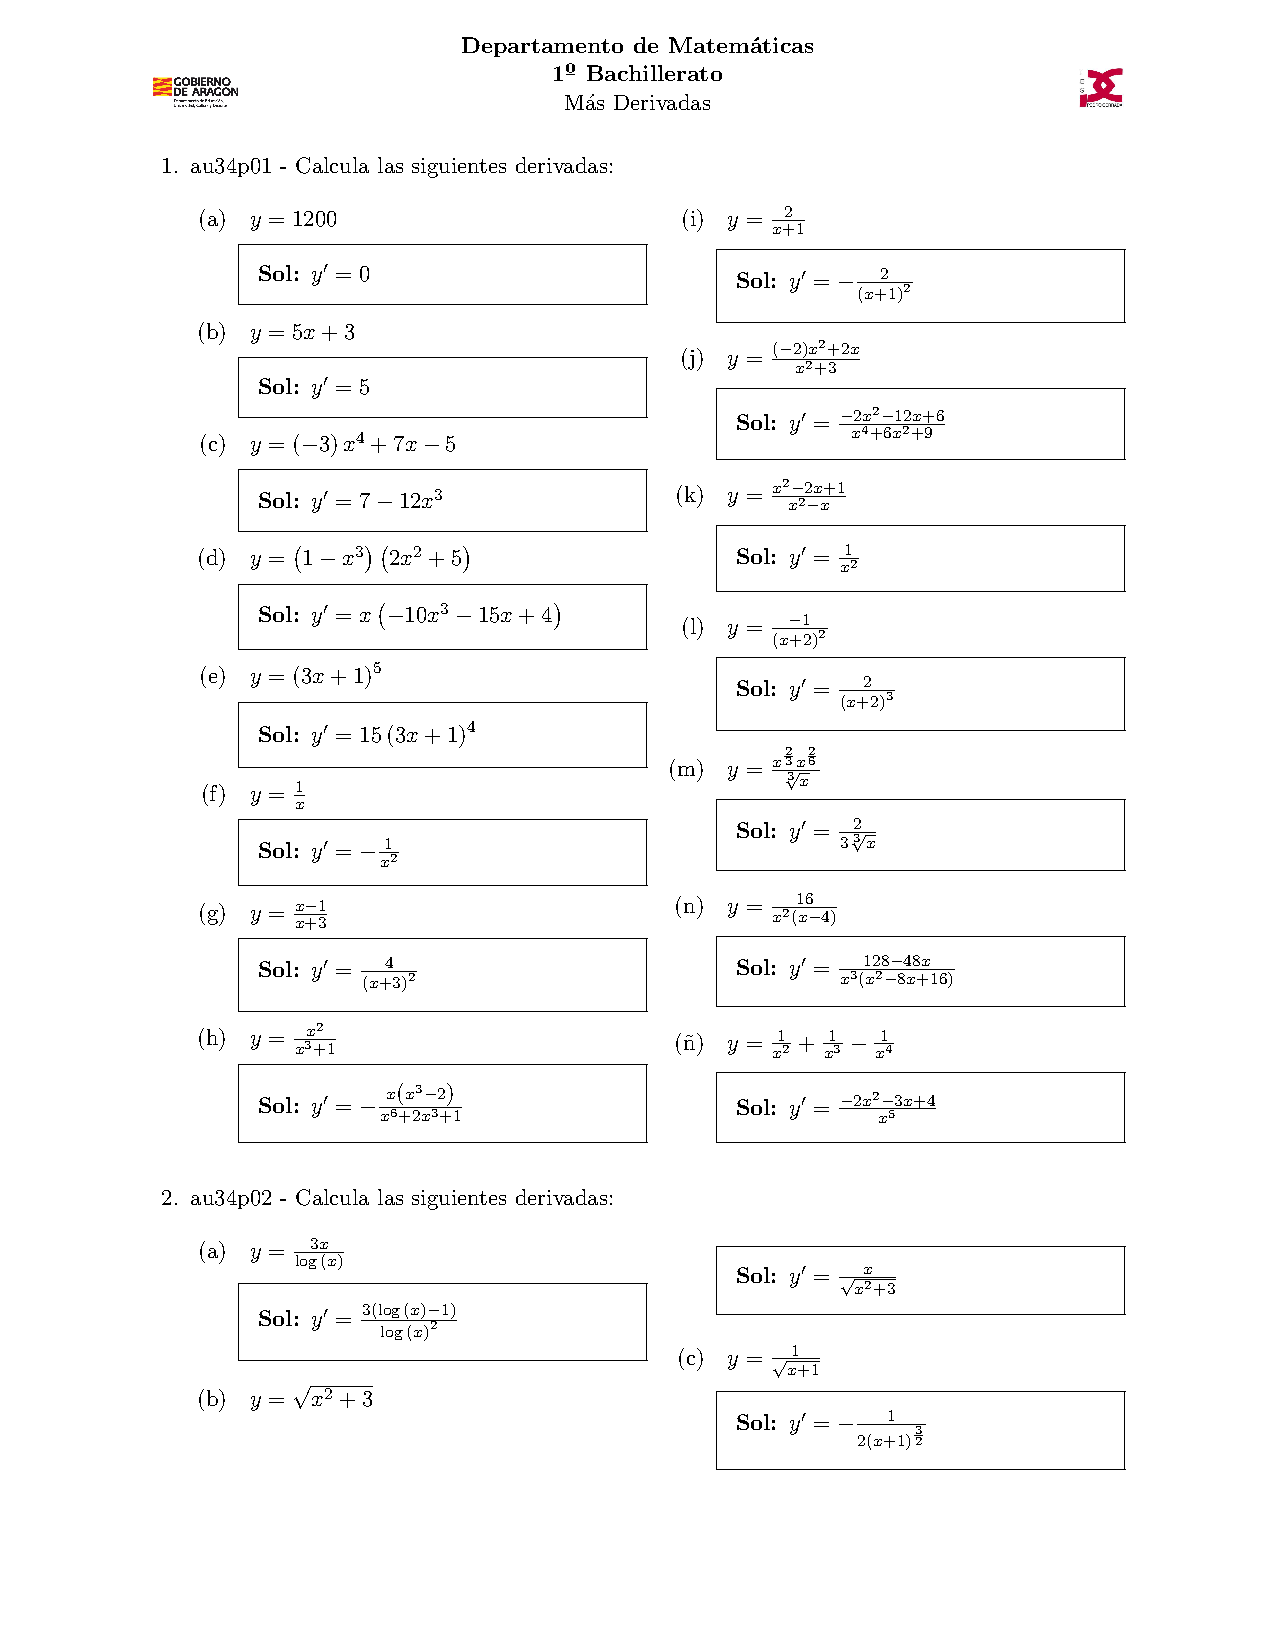
\includepdf[pages=-, scale=0.9]{4_analisis/34deriv2.pdf}
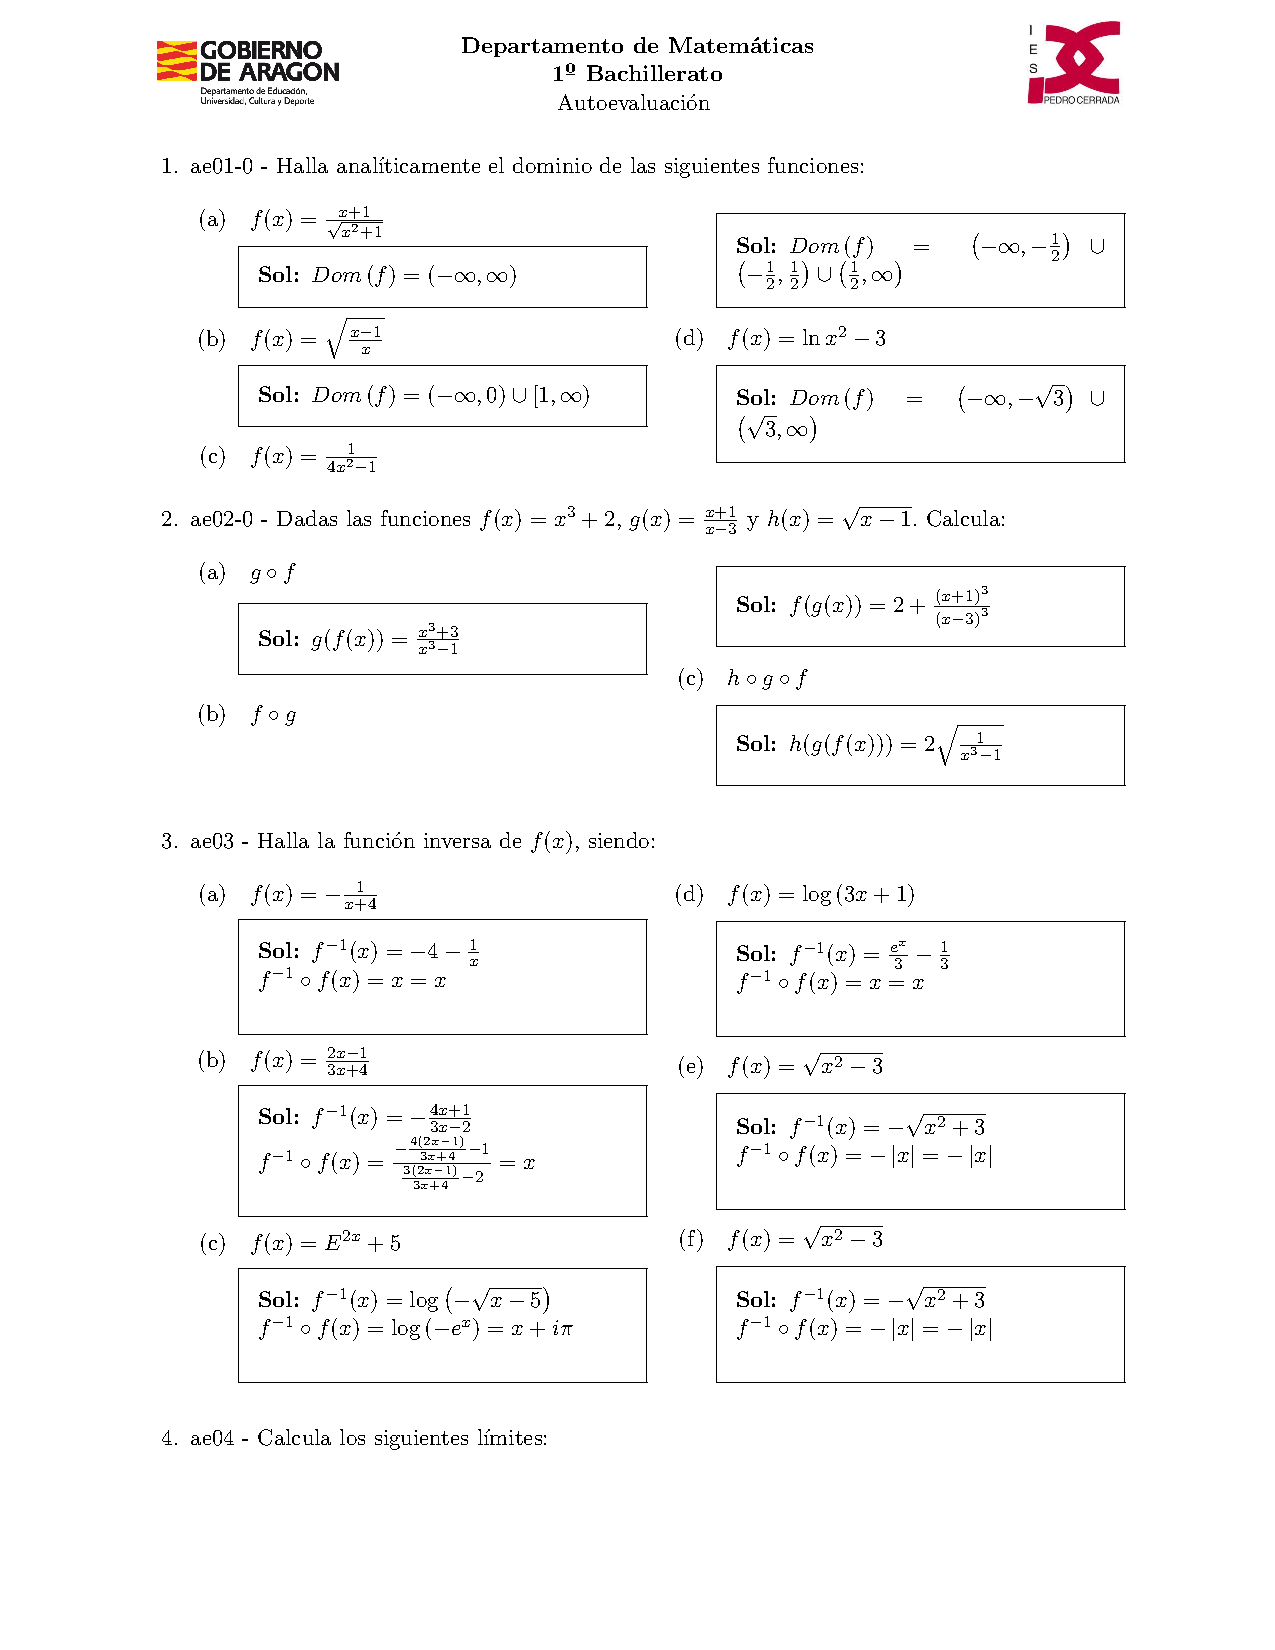
\includepdf[pages=-, scale=0.9]{4_analisis/autoev32.pdf}
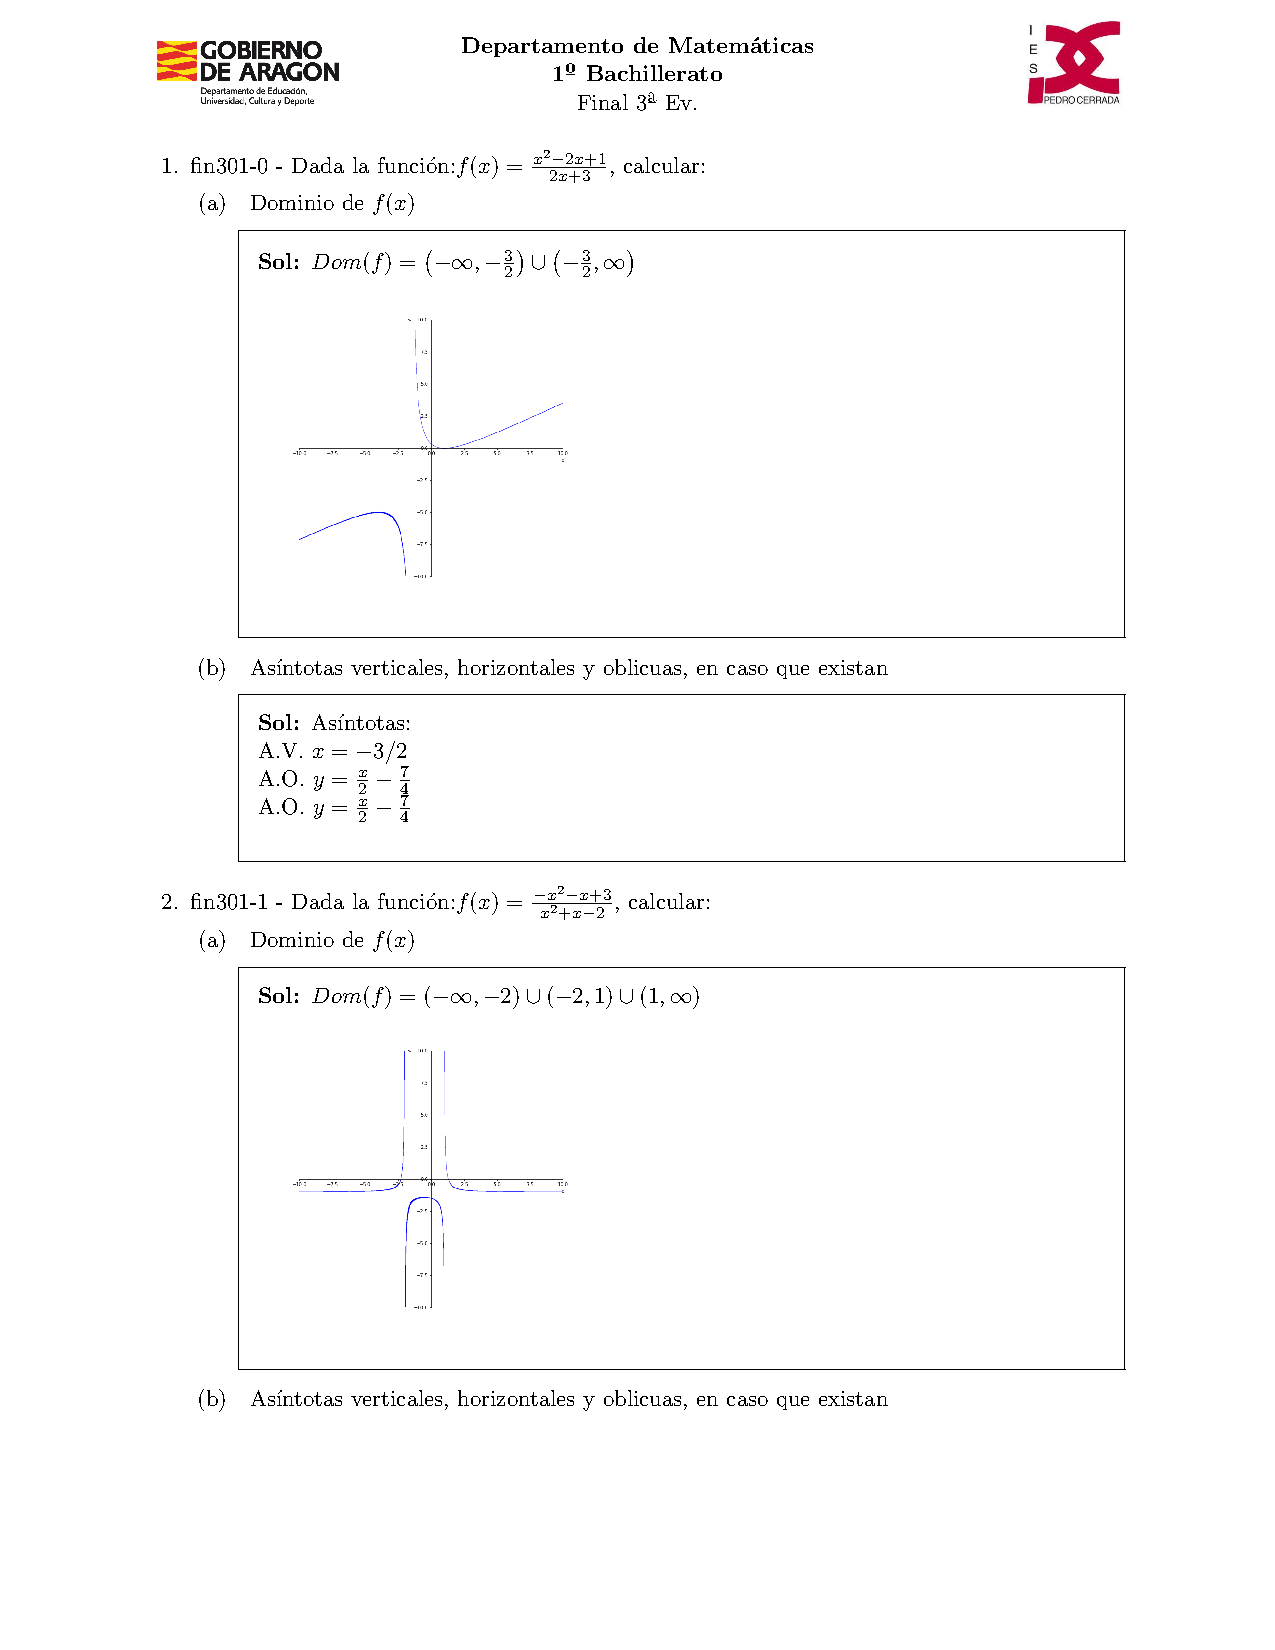
\includepdf[pages=-, scale=0.9]{4_analisis/autoev33.pdf}



\end{document}
